\documentclass[12pt]{book}
\usepackage[margin=0.8in]{geometry}
\parindent=0mm
\usepackage{tabularx,setspace, amssymb, amsmath, outlines, multicol, paralist, tikz, pgfplots, graphicx,enumitem, multienum, fixltx2e, fancyhdr,soul,lineno}
\pagestyle{fancy}
\everymath{\displaystyle}
\renewcommand{\indent}{\hspace{1cm}}
\newcommand{\longline}{\underline{\hspace{2in}} }
\newcommand{\shortline}{\underline{\hspace{1in}}}
\renewcommand{\baselinestretch}{1.15}
\newcommand{\medium}{\textbf{Medium} }
\newcommand{\basic}{\textbf{Basic} }
\newcommand{\advanced}{\textbf{Advanced} }
\newcommand{\plane}{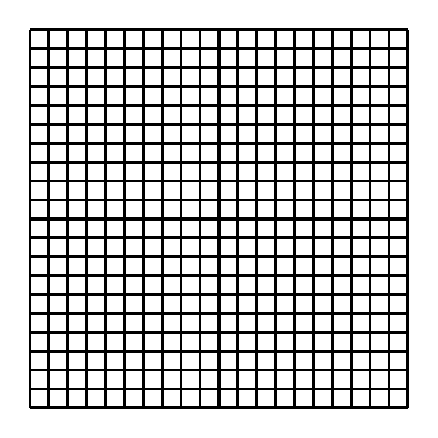
\begin{tikzpicture}[scale=0.6]
\draw[step=0.5] (0,0) grid (10,10);
\draw[ultra thick] (0,5) -- (10,5);
\draw[ultra thick] (5,0) -- (5,10);
\end{tikzpicture}}
\renewcommand*\tfrac[2]{
  \raisebox{-1em}{$\stackrel{\hbox{\underline{\smash{#1}}}}{\hbox{#2}}$}
}
\tikzset{every picture/.style={font issue=\footnotesize, scale=0.8},
	font issue/.style={execute at begin picture={#1\selectfont}},
	every path/.append style={line width=1 pt}
}

\lfoot{\raisebox{-.25\height}{
\includegraphics[scale=0.1]{logo}}{ \raisebox{0.25\height}{\small\copyright}\ Academic Student Center}}

\title{\textbf{\huge SAT Workbook}}
\author{
\includegraphics{logo}\\\textbf{\large ASC English}}
\date{}

\pgfplotsset{ every non boxed x axis/.append style={x axis line style=latex-latex}, every non boxed y axis/.append style={y axis line style=latex-latex},
axis x line=center, axis y line=center,
xmin=-5, xmax=5, ymin=-5, ymax=5,
axis line style = ultra thick, ticks=none,}

\begin{document}
\maketitle

\newpage
\vspace*{1em}

\vfill
\begingroup
\fontsize{10pt}{12pt}\selectfont
Copyright \copyright 2014 by ASC English and ISSC Management Company, Inc. All rights reserved.

\bigskip
In consuming this manual, ASC English teachers, students, staff, and their affiliates agree to not reproduce this manual. No part of this manual may be reproduced for distribution to a third part by any person, in any form, or by any means without the expressed, written consent of the publisher, ASC English. Distribution and/or copying includes, but is not limited to, electronic or mechanical distribution, such as photocopying, recording, or information retrieval system. Violators of this policy will be prosecuted to the fullest extent of the law.\\
 
\bigskip
The SAT is a registered trademark of the College Board. ASC English is not affiliated with the College Board. 

\bigskip
For more information about ASC English classes or publications, please call 617-730-3705 or go to our website, http:\//\//www.aplusprogram.com\//test\_prep\//sat.html

\bigskip
ASC English acknowledges the following authors and consultants for their contributions to this manual: Carl and Annie Nelson, ASC English; Lauren Blake, University of Chicago; Rebecca Safier, Harvard University; Richard Torres, Harvard University; Ben Letham, Massachusetts Institute of Technology (MIT); Nielson Phu, The College Panda; Jared Barbaresi, Connecticut College.  
\endgroup

\tableofcontents
\chapter{Introduction}

ASC's SAT Advanced course is designed to help students master the most difficult topics on the SATs. By focusing on and practicing these topics, advanced SAT students can improve their SAT scores.

\bigskip
The SAT is composed of ten sections—a 25-minute essay, six 25-minute sections, two 20-minute sections, and one 10-minute section. Total testing time is 3 hours and 45 minutes. The breakdown of each section is as follows:

\vfill
\newpage
\begin{spacing}{1.25}
\begin{tabularx}{\textwidth}{|*4{@{ }>{\raggedright\arraybackslash}X|}}\hline
\centerline{\textbf{Topic}} & \centerline{\textbf{Testing Time}} & {\textbf{Number of Questions}} & \centerline{\textbf{Skills Tested}}\\\hline
Critical Reading & Two 25 minute sections and one 20 minute section & 67 Questions in total: 19 sentence completions and 48 passage based questions & Vocabulary, sentence logic, answering questions and making inferences about a text\\\hline
Math & Two 25 minute sections and one 20 minute section & 54 Questions in total: 44 multiple choice and 10 student-produced responses & Integrating and applying mathematical concepts, including algebra, functions, geometry, probability, statistics, and data interpretation\\\hline
Writing Multiple Choice & One 25 minute section and one 10 minute section & 49 Questions in total: 25 Improving sentences, 18 identifying sentence errors, and 6 improving paragraph questions & Sentence structure and grammar, coherence and cohesion\\\hline
Writing Essay & 25 minutes & Write one essay on a given topic & Writing and analysis skills\\\hline
\end{tabularx}
\end{spacing}

\bigskip
You should also be aware that SAT test includes one 25-minute section called the “experimental section”. It can be in critical reading, math, or writing and is used by the testmakers to design and test questions for future exams. This section does not contribute to your SAT score, however, you won't know which section is the “experimental section”, so you should try your best on every part of the exam.

\bigskip
\underline{SAT Scoring}

Each section (critical reading, math, and writing) is scored by giving you a raw score and then converting that to a scaled score. The raw score is the number of questions that you got correct minus one-fourth of the questions that you got wrong. Leaving a question blank does not affect your score. This equation can be seen as:

\bigskip
\textbf{Raw Score: \underline{\hspace{1in}} correct $\boldsymbol{-}$ 0.25 (\underline{\hspace{1in}}) incorrect = \underline{\hspace{1in}}}

\bigskip
The raw score is then converted to a scaled score between 200 and 800 points. It should be noted that in the writing section, essay score is also factored into your scaled score. Additionally, in the math section, correct student-produced responses (grid ins) are worth one raw score point whereas incorrect student-produced responses (grid ins) do not affect your score.

\bigskip
This brings us to two very important questions:

\bigskip
\begin{inparaenum}[\bfseries1. ]
\item \textbf{If wrong answers lead to subtracting points, but a blank does not affect my score, should I guess?}

\bigskip
The answer is, it depends. If you are able to eliminate at least one choice, then the long run average results in the same or greater raw score than if you didn't guess. This also depends on the individual test taker's personality. Someone that tends to be more cautious might be tempted to leave a lot more blank than one should. On the other hand, a person that is more risk-inclined may have a tendency of not leaving enough blank. Therefore, if you are unsure, then you should complete a practice section leaving a few blank and guessing on the majority of questions that you don't know for sure and find your raw score using the equation above. Then, calculate what your raw score would have been had you left more of the ones that you were unsure of blank. Use whatever strategy gives you the highest score.


\bigskip
\item \textbf{What is a ``good'' SAT score?}
\end{inparaenum}

\bigskip
Although many people know that the coveted 2400 is a perfect score on the SATs, many students and parents wonder what other scores are classified as ``good''. This question does not have a simple answer because a ``good'' SAT score for one college might not be ``good'' for a more competitive school. For example, the top schools in the country tend to look for scores at least in the 700s in each of the three sections (2100 total), whereas smaller, less competitive schools will accept lower scores. While it is true that the higher a student's SAT scores are, the more opportunities will be available to a student, there are schools for students with a large range of SAT scores. Fortunately, there are tools to help students figure out their SAT score goal and what is a ``good'' score for their ability level and the colleges that they are hoping to gain acceptance from.

\bigskip
So what is a “good” score on the SAT? The answer is: it depends on what schools and, in some cases, what programs of study a student is aiming for. Therefore, first step in deciding what a “good score” is would be to decide what colleges or universities interest you and come up with a few ideas of what you might want to study. Next, just check online what scores your ideal school is looking for and make it your goal to score a bit higher just so you stand out among all the other applicants. Oftentimes, the university's website will contain the average SAT score and GPA for admitted applicants. They might also give a 25\% to 75\% percentile scores. Someone in this range might be a good match for the school, whereas it might be more difficult for someone with SAT scores than the 25\% percentile to be admitted. The College Board (the same company that makes the SATs) also has an online program called ``My College Matches'' to help students identify colleges that might be good for them sorted by individual factors such as SAT score. Identifying potential areas of study could also help to put SAT scores in context. For example, a student who scores a 2100 by getting 800s on the verbal and reading section and a 500 on math might make it into a writing program at a top university but would not be considered by a high ranking technical institution. Every school and every student's situations are different.

\newpage
\textbf{\large About the Critical Reading Section}

The critical reading section is composed of two parts, sentence completions and passage-based reading. The sentence completion focuses on vocabulary and sentence logic in order to select the word that best fits in the blank within the sentence. It is imperative that students learn to detect the types of sentence completions and the clues given in each of the sentences which will lead to the correct answer. For the passage-based reading, students will learn the types of passages and questions tested as well as strategies for detecting the correct answer and the reasons that incorrect answers are incorrect.

\bigskip
\textbf{\large About the Math Section}

The following topics are tested on the SAT math section: number and operations, algebra and functions, geometry and measurement, and data analysis, statistics, and probability questions. 

\bigskip
Below is a list from the College Board of each topic tested in more detail:

\bigskip
\begin{outline}
\0 \underline{Number and Operations ($20-25$\% of the test)}
\1 Arithmetic word problems (including percent, ratio, and proportion)
\1 Properties of integers (even, odd, prime numbers, divisibility, and so forth)
\1 Rational numbers
\1 Sets (union, intersection, elements)
\1 Counting techniques
\1 Sequences and series (including exponential growth)
\1 Elementary number theory
\0 \underline{Algebra and functions questions ($35-40$\% of the test)}
\1 Substitution and simplifying algebraic expressions
\1 Properties of exponents
\1 Algebraic word problems
\1 Solutions of linear equations and inequalities
\1 Systems of equations and inequalities
\1 Quadratic equations
\1 Rational and radical equations
\1 Equations of lines
\1 Absolute value
\1 Direct and inverse variation
\1 Concepts of algebraic functions
\1 Newly defined symbols based on commonly used operations
\0 \underline{Geometry and measurement questions ($25-30$\% of the test)}
\1 Area and perimeter of a polygon
\1 Area and circumference of a circle
\1 Volume of a box, cube, and cylinder
\1 Pythagorean theorem and special properties of isosceles, equilateral, and right triangles
\1 Properties of parallel and perpendicular lines
\1 Coordinate geometry
\1 Geometric visualization
\1 Slope
\1 Similarity
\1 Transformations
\0 \underline{Data analysis, statistics, and probability questions ($10-15$\% of the test)}
\1 Data interpretation (tables and graphs)
\1 Descriptive statistics (mean, median, and mode)
\1 Probability
\end{outline}

You will note that there is no pre-calculus or advanced trigonometry (sine, cosine, tangent, etc.), so if you haven't taken these classes, don't worry about it. However, you should be cognizant of when you took what classes and, consequently how much time that you will need to focus on each topic. For example, an 11th grader that took geometry in 9th grade may need to spend more time reviewing geometry than a 11th grader that is currently in a geometry class.

\bigskip
\textbf{\large About the writing section}

The writing section is composed of two sections, the 25 minute essay and multiple choice questions. Students will learn what the SAT graders are looking for and also practice with timing, brainstorming, and writing so that they can get a perfect score on the essay. Students will also be exposed to the three types of writing multiple choice questions-- sentence improvements, sentence errors, and paragraph improvements—as well as the grammatical or other writing concepts taught in this section.

\newpage
\centerline{\textbf{SAT Homework Agenda}}

\bigskip
\begin{spacing}{1.5}
\begin{tabularx}{\textwidth}{|*3{@{}>{\bfseries\centering\arraybackslash}X|}}\hline
Date Due & SAT Verbal & SAT Math\\\hline
& & \\[8ex]\hline
& & \\[8ex]\hline
& & \\[8ex]\hline
& & \\[8ex]\hline
& & \\[8ex]\hline
& & \\[8ex]\hline
& & \\[8ex]\hline
& & \\[8ex]\hline
& & \\[8ex]\hline
\end{tabularx}
\end{spacing}


\part{SAT Math}
\chapter[SAT Geometry]{Strategies for SAT Geometry}

\section{SAT Worksheet 1A: Warm-Up Problems}

\textbf{Strategies practice:} Draw a diagram and any information that you can described in each of the following questions

\begin{multienumerate}
\mitemxx{Points $A, B$, and $C$ are colinear and line $D$ is perpendicular to point $A$. Line $E$ is parallel to line $D$.}
{In right triangle $ABC$, point $D$ is equidistant to points $A$ and $B$ on the hypotenuse, line $AB$.}
\end{multienumerate}

\vfill
\hrulefill

\textbf{Content Practice:} The following is designed to ensure that you have a proper grasp of the concepts that you will see on the SAT math section. Read the words and definitions (if you don't already know them) and then answer the question that follows.

\bigskip
\begin{enumerate}[label=\bfseries\arabic*.]
\item \textbf{Whole Numbers, Integer, Decimal, Real Number} $-$ A whole number is any non-decimal, non-negative number (0 included). An integer is any non-decimal number, positive, negative, or 0. A decimal is a part of another number. A real number is a number that exists in the real plane instead of the imaginary.

\bigskip
\indent Identify the following numbers: $2, 0, -1, 0.25, i$

\vfill\item \textbf{Remainder} $-$ The amount left over after a long division. What is the remainder of the quotient of 20 and 2?

\vfill
\newpage
\item \textbf{Numerator/Denominator} $-$ The numerator is the number on top of a fraction. The denominator is the number on the bottom. If a fraction has a numerator of four and a denominator of five, what is its value as a decimal?

\vfill\item \textbf{Absolute Value} $-$ The distance away of a number from 0. It will always be represented as a positive number. Absolute value is represented by $|x|$.

\bigskip
\indent Evaluate the following: $|-3|+|6|\times|8|-|-15|$

\vfill\item \textbf{Sum, difference, product, quotient} $-$ The sum is the result of adding two numbers. The difference is the result of subtracting two numbers. The product is the result of multiplying two numbers. The quotient is the result of dividing two numbers.

\bigskip
\indent Find the sum, difference, product, and quotient of 15 and 5.

\vfill\item \textbf{Operation} $-$ A set of rules to explain what must the computation to be performed on two or more values

\bigskip
\indent Let the operation $x@y$ be equal to $3x+2y$. Evaluate $5@8$.

\vfill\item \textbf{Multiple, factor, prime, divisible by} $-$ A multiple is a number that can be divided by (is divisible by) another without a remainder. A factor is a number that can be used to divide another number without a remainder. A factor is anumber that can be used to divide another number without a remainder. A prime number is a number that cannot be divided by any number (except 1) without a remainder.

\bigskip
\indent List 5 multiples of 6.

\bigskip
\indent List all the positive factors of 60

\vfill\item \textbf{Consecutive} $-$ One right after another. The sum of 3 consecutive numbers is 21. What is the value of the largest number?

\vfill\item \textbf{Distinct} $-$ Different

\vfill
\newpage
\underline{Geometry Vocabulary}

\medskip
\item \textbf{Bounded} $-$ Restrained or bordered by

\bigskip
Shade in the region bound by the lines $y=2, y=2x+2$, and $y=-2x+4$ then find the three points that are the vertices of the shaded region.

\bigskip
\centerline{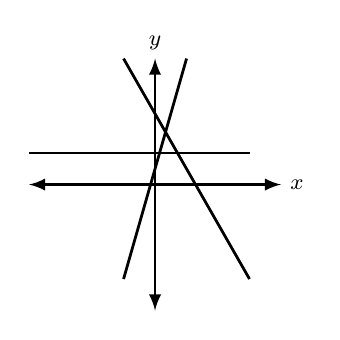
\begin{tikzpicture}
\draw [latex-latex] (0,2) -- (4,2) node[anchor=west] {$x$};
\draw [latex-latex] (2,0) -- (2,4) node[anchor=south] {$y$};
\draw (0,2.5) -- (3.5,2.5);
\draw (1.5,4) -- (3.5,0.5);
\draw (1.5,0.5) -- (2.5,4);
\end{tikzpicture}}

\vfill\item \textbf{Lie in a plane} $-$ Something that lies within a plane is located within the boundaries of said plane

\bigskip
State which points do an which points do not lie in plane $A$

\bigskip
\centerline{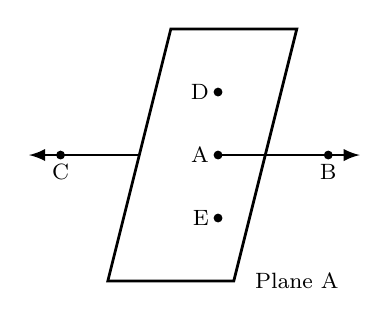
\begin{tikzpicture}
\draw (0,0) -- (2,0) -- (3,4) -- (1,4) -- cycle;
\draw [-latex] (1.75,2) -- (4,2);
\draw [latex-] (-1.25,2) -- (0.5,2);
\fill (-0.75,2) node[anchor=north] {C} circle (2pt);
\fill (3.5,2) node[anchor=north] {B} circle (2pt);
\fill (1.75,2) node[anchor=east] {A} circle (2pt);
\fill (1.75,3) node[anchor=east] {D} circle (2pt);
\fill (1.75,1) node[anchor=east] {E} circle (2pt);
\draw (3,0) node {Plane A};
\end{tikzpicture}}

\vfill\item \textbf{Acute, Right, Obtuse} $-$ An acute angle is less than 90 degrees. A right angle is exactly 90 degrees. An obtuse angle is larger than 90 degrees.

\bigskip
Identify the type of angle:

\begin{center}
\begin{multicols}{3}
\begin{tikzpicture}
\draw (0,2) -- (2,0) -- (4,0);
\draw (2,-0.5) node {A};
\end{tikzpicture}


\columnbreak
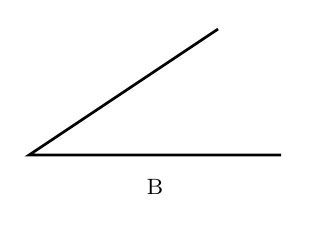
\begin{tikzpicture}
\draw (3,2) -- (0,0) -- (4,0);
\draw (2,-0.5) node {B};
\end{tikzpicture}


\columnbreak
\begin{tikzpicture}
\draw (0,2) -- (0,0) -- (2,0);
\draw (0,0.5) -- (0.5,0.5) -- (0.5,0);
\draw (1,-0.5) node {C};
\end{tikzpicture}
\end{multicols}
\end{center}

\vfill
\newpage
\item \textbf{Equilateral, Isosceles, Scalene} $-$ An equilateral triangle has three equal sides. An isosceles triangle has two equal sides. A scalene triangle has no equal sides.

Identify the type of triangle:

\begin{multicols}{3}
\begin{center}
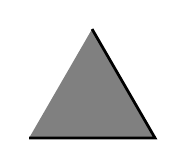
\begin{tikzpicture}
\draw[fill=gray] (0,0) -- (2,0) -- (1,1.73);
\draw (0,0);
\end{tikzpicture}

A
\end{center}

\columnbreak
\begin{center}
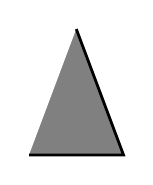
\begin{tikzpicture}
\draw[fill=gray] (0,0) -- (1.5,0) -- (0.75,2);
\end{tikzpicture}

B
\end{center}

\columnbreak
\begin{center}
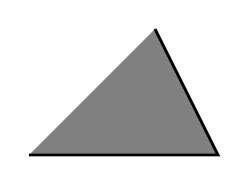
\begin{tikzpicture}
\draw[fill=gray] (0,0) -- (3,0) -- (2,2);
\end{tikzpicture}

C
\end{center}
\end{multicols}

\vfill\item \textbf{Shaded region} $-$ The area of the figure with a dark gray coloring

\bigskip
Find the area of the shaded region within the square

\begin{center}
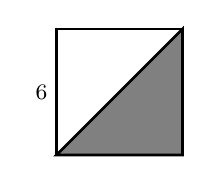
\begin{tikzpicture}
\draw (0,0) -- (2,0) -- (2,2) -- (0,2) -- cycle;
\draw[fill=gray] (0,0) -- (2,0) -- (2,2) -- cycle;
\draw (0,1) node[anchor=east] {6};
\end{tikzpicture}
\end{center}

\vfill\item \textbf{Parallel} $-$ Two lines that never intersect

\bigskip
Give an example of an equation of the line that is parallel to $y=3x+7$

\begin{center}

\begin{tikzpicture}
\draw (0,0) -- (2,2);
\draw (1,0) -- (3,2);
\end{tikzpicture}
\end{center}

\vfill\item \textbf{Perpendicular} $-$ Two lines that intersect to form a right angle

\bigskip
White two lines below are perpendicular? \underline{\hspace{1in}}

\bigskip
\centerline{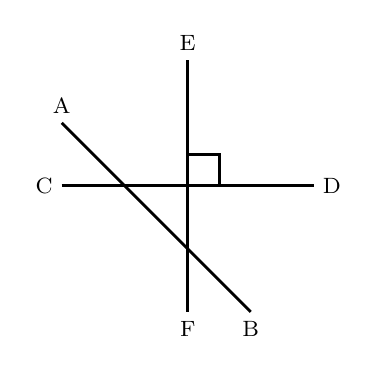
\begin{tikzpicture}
\draw (0,2) node[anchor=east] {C} -- (4,2) node[anchor=west] {D};
\draw (0,3) node[anchor=south] {A} -- (3,0) node[anchor=north] {B};
\draw (2,0) node[anchor=north] {F} -- (2,4) node[anchor=south] {E};
\draw (2, 2.5) -- (2.5,2.5) -- (2.5,2);
\end{tikzpicture}}

\vfill\item \textbf{Tangent} $-$ A line that intersects at exactly one point on a circle

\bigskip
Which line is tangent to circle $R$?

\begin{center}
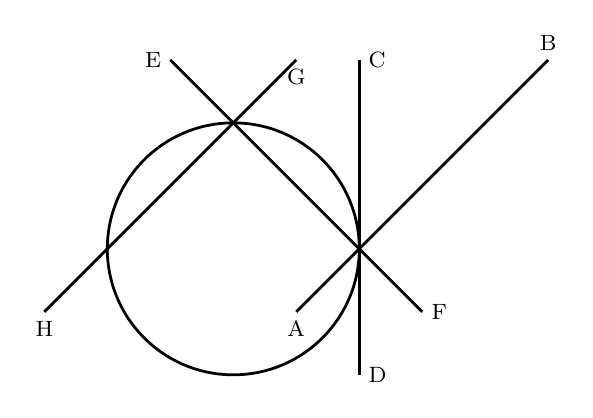
\begin{tikzpicture}
\draw (3,3) circle (2cm);
\draw (0,2) node[anchor=north] {H} -- (4,6) node[anchor=north] {G};
\draw (5,6) node[anchor=west] {C} -- (5,1) node[anchor=west] {D};
\draw (4,2) node[anchor=north] {A} -- (8,6) node[anchor=south] {B};
\draw (2,6) node[anchor=east] {E} -- (6,2) node[anchor=west] {F};
\end{tikzpicture}
\end{center}
\end{enumerate}

\vfill
\newpage
\section[General Strategies]{General Strategies for the SAT Geometry Section}

\bigskip
\textbf{Strategy \#1: Visualization is key!} As we saw in the strategy section of the warm-up, \longline can help to break up complex language and also to give you a jumping off point to start solving the problem. If the SAT problems give you a diagram as part of the problem, then you should always start by marking the information given or that you can directly deduce directly onto the image.

\bigskip
\textbf{Strategy \#2: Minimize the number of variables!} Not having numbers at the onset of a problem can increase the difficulty level of the SAT problem, particularly the geometry problems. Therefore, if you can covert these relationships or variables to \underline{\hspace{1.5in}}, then it is easier to think about and solve the problem.

\bigskip
One way to do this: Whenever there is a relationship between two objects (angles, line segments, etc.), you are probably going to need to numerically solve for this relationship. This will either be your answer or it will directly be used to find your answer. Therefore, if you see a ratio in the problem, then convert it to variables and solve for the variables if possible. If you can convert a line segment to a number line with numerical distances, then do it!

\vfill
\newpage
\section{Distances on a Line}

\bigskip
Examples:

\begin{multicols}{2}
\begin{enumerate}[label*=\arabic*.]
\item \textbf{Medium}

In the $xy$-coordinate plane, point $A$ is at $(1,5)$ and point $B$ is at $(-a,-3)$. The distance between points $A$ and $B$ is 12. What is the value of $a$?
\vfill
\phantom{}
\columnbreak
\item \textbf{Medium}

Lines $l, m,$ and $r$ are all different lines that lie in the same plane. If $l\perp m, m\perp r$, and $r\perp s$, which of the following must be true?

\bigskip
\begin{enumerate}[label=\Roman*.]
\item $l\perp s$
\item $l\parallel r$
\item $m\perp s$
\end{enumerate}

\begin{enumerate}[label=(\Alph*)]
\item I only
\item I and II only
\item I and III only
\item II and III only
\item I, II, and III
\end{enumerate}
\end{enumerate}
\end{multicols}

\vfill
Problem solving strategy for distances on a line:

\begin{spacing}{1.5}
\begin{enumerate}[label=\Roman*)]
\item \longline if one doesn't exist
\item \longline the diagram (what is equal to what, etc). Convert it to a

\longline if possible
\item Solve for the \longline of the different segments
\item Use the information in steps \#$1-3$ to \longline
\end{enumerate}
\end{spacing}

\vfill
\newpage
\section{SAT Worksheet 2A: 6, Questions, 8 Minutes}


\begin{multienumerate}
\mitemxx{\basic

\begin{center}
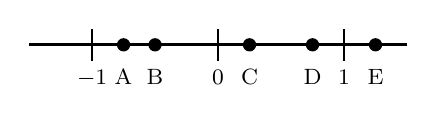
\begin{tikzpicture}
\draw (0,1) -- (6,1);
\draw (1,1.25) -- (1,0.75) node[anchor=north] {$-1$};
\fill (1.5,1) circle(3pt);
\draw (1.5,0.75) node[anchor=north] {A};
\fill (2,1) circle(3pt);
\draw (2,0.75) node[anchor=north] {B};
\draw (3,1.25) -- (3,0.75) node[anchor=north] {0};
\fill (3.5,1) circle(3pt);
\draw (3.5,0.75) node[anchor=north] {C};
\fill (4.5,1) circle(3pt);
\draw (4.5,0.75) node[anchor=north] {D};
\draw (5,1.25) -- (5,0.75) node[anchor=north] {1};
\fill (5.5,1) circle(3pt);
\draw (5.5,0.75) node[anchor=north] {E};
\end{tikzpicture}
\end{center}

Given the points on the number line above, which product has the smallest value?

\begin{enumerate}[label=(\Alph*)]
\item $A\times B$
\item $A\times C$
\item $B\times D$
\item $D\times E$
\item $B\times C$
\end{enumerate}}
{\basic

Points $P, Q, R,$ and $S$ lie on a line, in that order, so that $Q$ is the midpoint of $PR$, $R$ is the midpoint of $QS$, and $PS=18$. If point $X$ lies between $Q$ and $R$ and $QX=4$, what is the length of $XS$?

\begin{enumerate}[label=(\Alph*)]
\item 2
\item 4
\item 6
\item 8
\item 10
\end{enumerate}}

\vfill
\mitemxx{\medium

\begin{center}
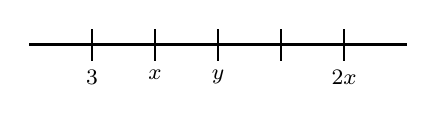
\begin{tikzpicture}
\draw (0,1) -- (6,1);
\draw (1,1.25) -- (1, 0.75) node[anchor=north] {3};
\draw (2,1.25) -- (2, 0.75) node[anchor=north] {$x$};
\draw (3,1.25) -- (3, 0.75) node[anchor=north] {$y$};
\draw (4,1.25) -- (4, 0.75);
\draw (5,1.25) -- (5, 0.75) node[anchor=north] {$2x$};
\end{tikzpicture}
\end{center}

In the number line above, the tick marks are equally spaced. What is the value of $y$?

\begin{enumerate}[label=(\Alph*)]
\item 5
\item 6
\item 7
\item 8
\item 9
\end{enumerate}}
{\medium

Points $X$ and $Y$ are two different points on a circle. Point $m$ is localed so that line segment $XM$ and line segment $YM$ have equal lengths. Which of the following could be true?

\begin{enumerate}[label=\Roman*.]
\item $M$ is on the center of the circle
\item $M$ is on the arc $XY$
\item $M$ is outside of the circle
\end{enumerate}

\begin{enumerate}[label=(\Alph*)]
\item I only
\item II only
\item I and II only
\item II and III only
\item I, II, and III
\end{enumerate}}

\vfill
\mitemxx{\advanced

$R$ is the midpoint of line segment $PT$ and $Q$ is the midpoint of line segment $PR$. If $S$ is a point between $R$ and $T$ such that the length of segment $QS$ is 10 and the length of segment $PS$ is 19, what is th length of $ST$?}
{\advanced

Point $M$ is the midpoint of line segment $AB$. Points $C$ and $D$ are located on $AB$ in such a way that $AC=CM$ and $MD=DB$. If $MD=5$, what is the length of $AD$?}
\end{multienumerate}

\vfill
\newpage
\section{Angles and Lines}

\bigskip
Examples:

\begin{multienumerate}
\mitemxx{\basic

\begin{center}
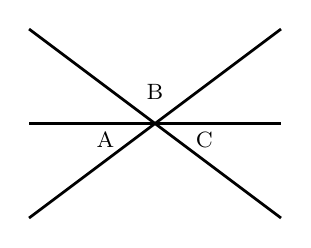
\begin{tikzpicture}
\draw (0,1.5) -- (4,1.5);
\draw (0,0) -- (4,3);
\draw (0,3) -- (4,0);
\draw (1.5,1.5) node[anchor=north east] {A};
\draw (2, 2) node {B};
\draw (2.5, 1.5) node[anchor=north west] {C};
\end{tikzpicture}
\end{center}

\bigskip
In the figure above, if $\angle A=50^\circ, \angle B=42^\circ$, and $\angle C=2x^\circ$, what is the measure of $\angle C$?

\begin{enumerate}[label=(\Alph*)]
\item $166^\circ$
\item $43^\circ$
\item $88^\circ$
\item $50^\circ$
\item $138^\circ$
\end{enumerate}
}{\medium

In the $xy$-plane, line $l$ is $2x-3y=5$. Which of the following coordinates are on a line perpendicular to line $l$ with a $y$-intercept of $-10$?

\begin{enumerate}[label=(\Alph*)]
\item $(-2,4)$
\item $(-6,-1)$
\item $(-6,-2)$
\item $(-2,-7)$
\item $(-1,-4.5)$
\end{enumerate}}
\end{multienumerate}

\hrulefill

What is the sum of angles of a straight line?

\begin{center}
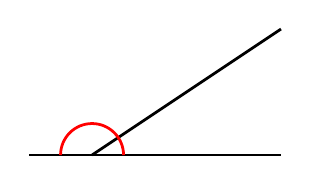
\begin{tikzpicture}
\draw (0,0) -- (4,0);
\draw (1,0) -- (4,2);
\draw[color=red] (1.5,0) arc (0:180:0.5);
\end{tikzpicture}
\end{center}

What is the sum of angles around two straight lines? In this case, which angles are congruent? Why?

\begin{center}
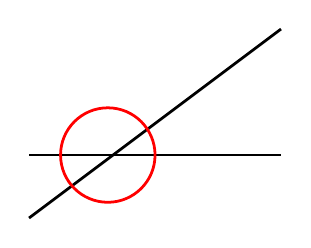
\begin{tikzpicture}
\draw (0,0) -- (4,0);
\draw (0,-1) -- (4,2);
\draw[color=red] (2,0) arc (0:360:0.75);
\end{tikzpicture}
\end{center}

In the figure to the right, lines $l$ and $m$ are parallel. Which angles or sums of angles are congruent? Which angles sum to $180^\circ$ and why?

\begin{center}
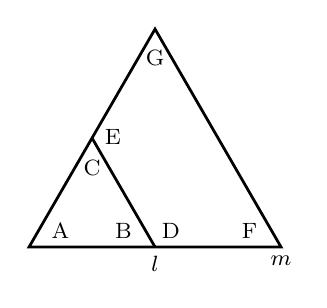
\begin{tikzpicture}
\draw (0,0) -- (4,0) node[anchor=north] {$m$} -- (2,3.46) -- cycle;
\draw (0.5,0.25) node {A};
\draw (1.5,0.25) node {B};
\draw (2.25,0.25) node {D};
\draw (3.5,0.25) node {F};
\draw (1,1.73) -- (2,0) node[anchor=north] {$l$};
\draw (1,1.25) node {C};
\draw (1.33,1.75) node {E};
\draw (2,3) node {G};
\end{tikzpicture}
\end{center}

Other questions will ask you about the slope of a line or about parallel or perpendicular lines.

\bigskip
\textbf{To find the slope of a line:} You need at least 2 points on the line. Write down the $x$ and $y$ coordinates for points 1 and 2. Then, slope = $(y_2-y_1)/(x_2-x_1)$.

\bigskip
\textbf{About parallel lines:} Parallel lines have the same slope. To find the equation of a line parallel to the given line, find the slope of the given line (see \#1). It is also the ``$m$'' term in the equation of a line, $y=mx+b$. Then, plug in $x$ and $y$ coordinates to the equation of a line with the same $m$ as the original line and solve for $b$.

\bigskip
\textbf{About perpendicular lines:} The slopes of perpendicular lines are negative reciprocals. To find the equation of a line perpendicular to a given line, Find the slope of the given line (see \#1). It is also the ``$m$'' term in the equation of a line, $y=mx+b$. Then, take it's negative reciprocal to find the slope for the perpendicular line. Plug in $x$ and $y$ coordinates to the equation of a line with the m that was solved for in the previous step. Solve for $b$.

\newpage
\subsection{SAT Worksheet 3A: 6 Questions, 8 Minutes}

\begin{multienumerate}
\mitemxx{\basic

\begin{center}
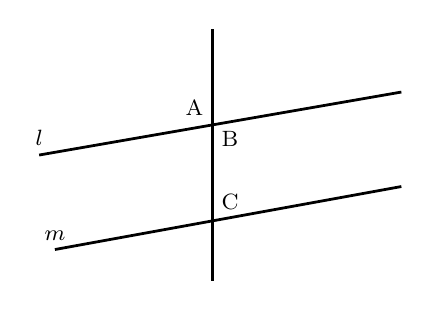
\begin{tikzpicture}
\draw (0.5,0.5) node[anchor=south] {$m$}-- (6,1.5);
\draw (0.25,2) node[anchor=south] {$l$} -- (6,3);
\draw (3,4) -- (3,0);
\draw (3,2.75) node[anchor=east] {A};
\draw (3,2.25) node[anchor=west] {B};
\draw (3,1.25) node[anchor=west] {C};
\end{tikzpicture}
\end{center}

If $l \parallel m, B=(x+5)^\circ$, and $C=(3x-17)^\circ$, what is the measurement of angle $A$?
}{\basic

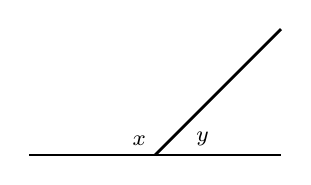
\begin{tikzpicture}
\draw (0,0) -- (4,0);
\draw (2,0) node[anchor=south east] {$x$} -- (4,2);
\draw (3,0) node[anchor=south east] {$y$};
\end{tikzpicture}

In the figure above, what is $y$ in terms of $x$?

\begin{enumerate}[label=(\Alph*)]
\item $90^\circ-x$
\item $90^\circ-x/2$
\item $90^\circ+x/2$
\item $120^\circ-x$
\item $180^\circ-x$
\end{enumerate}}

\mitemxx{\medium

\begin{center}
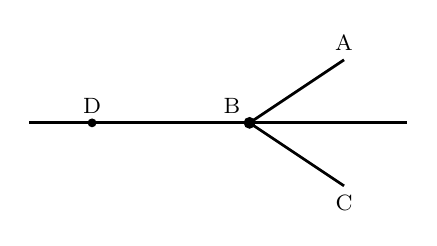
\begin{tikzpicture}
\draw (0,2) -- (6,2);
\fill (1,2) node[anchor=south] {D} circle (2pt);
\draw[fill=black] (5,1) node[anchor=north] {C} -- (3.5,2) node[anchor=south east] {B} circle (2pt) -- (5,3) node[anchor=south] {A};
\end{tikzpicture}
\end{center}

If line A bisects $\angle ABC$, and the measure of $\angle ABC$ is $80^\circ$, what is the value of $\angle CBD$?
}{\medium

\begin{center}
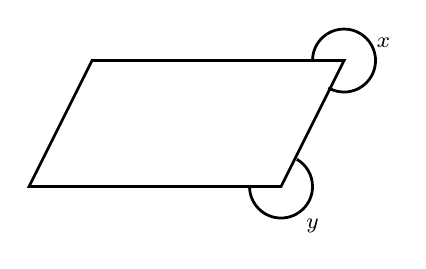
\begin{tikzpicture}
\draw (0,0) -- (4,0) -- (5,2) -- (1,2) -- cycle;
\draw (3.5,0) arc (180:420:0.5);
\draw (4.5,-0.625) node {$y$};
\draw (4.5,2) arc (180:-120:0.5);
\draw (5.625,2.275) node {$x$};
\end{tikzpicture}
\end{center}

The figure above is a parallelogram. If $x=300^\circ$, what is the value of $y$?

\begin{enumerate}[label=(\Alph*)]
\item $200^\circ$
\item $240^\circ$
\item $280^\circ$
\item $320^\circ$
\item $330^\circ$
\end{enumerate}}

\mitemxx{\advanced

The measure of the largest angle in a certain triangle is twice the sum of the measures of the remaining angles. What is the measure of the largest angle?

\begin{enumerate}[label=(\Alph*)]
\item $45^\circ$
\item $60^\circ$
\item $90^\circ$
\item $120^\circ$
\item $150^\circ$
\end{enumerate}
}
{\advanced

The line in the $xy$-plane that contains the points $(2, 5)$ and $(4, y)$ has slope 0. What is the value of $y$?}
\end{multienumerate}

\newpage
\textbf{\large Triangles}

\bigskip
Examples

\begin{multienumerate}
\mitemxx{\basic

\begin{center}
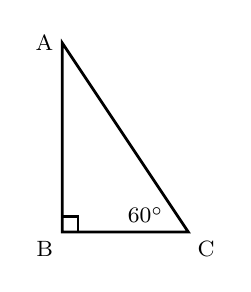
\begin{tikzpicture}
\draw (0,0) node[anchor=north east] {B} -- (2,0) node[anchor=north west] {C} -- (0,3) node[anchor=east] {A} -- cycle;
\draw (0,0.25) -- (0.25,0.25) -- (0.25,0);
\draw (1.75,0) node[anchor=south east] {$60^\circ$};
\end{tikzpicture}
\end{center}

If $AB=8$, what is the length of $AC$?
}{\medium

\begin{center}
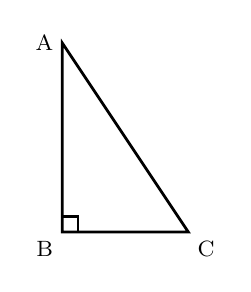
\begin{tikzpicture}
\draw (0,0) node[anchor=north east] {B} -- (2,0) node[anchor=north west] {C} -- (0,3) node[anchor=east] {A} -- cycle;
\draw (0,0.25) -- (0.25,0.25) -- (0.25,0);
\end{tikzpicture}
\end{center}

If $AB=BC=4/11$, what is the value of $AC$? What is the value of $x$?
}
\end{multienumerate}

\hrulefill

There are two main types of questions with triangles on the SATs that involve triangles: solving for angles in a triangle and solving for a side length of a triangle. Many of these will involve special right triangles.

\bigskip
Solving for side lengths: You will primarily use the Pythagorean theorem and Pythagorean triples, rules of special right triangles, and rules of the lengths of a triangle. 

\bigskip
\begin{enumerate}[label=\arabic*)]
\item What is the general rule for the lengths of the side lengths of a triangle?
\vfill\item What are Pythagorean triples? In what types of problems can they be used on the SAT?
\vfill\item What are examples of Pythagorean triples? The most commonly used Pythagorean triples on the SAT are \longline
\vfill\item What are the rules for side lengths of $30^\circ-60^\circ-90^\circ$ special right triangles?
\vfill\item What are the rules for side lengths of $45^\circ-45^\circ-90^\circ$ special right triangles?
\end{enumerate}

\vfill
\newpage
\textbf{\large Complex Polygons}

There are many types of problems with angles in triangles and more complex shapes. Many will ask students to integrate knowledge of the types of angles (of triangles and n-shaped polygons) and straight, parallel and perpendicular lines. 

\bigskip
\begin{enumerate}[label=\arabic*)]
\item What is the general formula for the sum of the interior angles of a n-sided polygon?
\vfill\item What is the sum of the interior angles of a quadrilateral?
\vfill\item What is the sum of the interior angles of a pentagon?
\vfill\item What is the sum of the interior angles of a hexagon?
\vfill\item What is the sum of the interior angles of an octagon?
\end{enumerate}

\vfill
\section[Complex Polygons]{General Strategies for Finding Angles in a Complex Polygon}

\bigskip
\begin{enumerate}[label=\arabic*)]
\item Identify the large polygon(s) and the polygons within the main polygon. Try to fill in \longline that you do know based on the sum of interior angles of a triangle, quadrilateral, or other polygons in the problem.

\bigskip\item Try to fill in angles that you do know using properties of \longline

\bigskip\item Then try to put the information from steps 1 and 2 together to try to solve for more angles in the polygon and eventually the angle or variable that you are looking for. 
\end{enumerate}

\newpage
\subsection{SAT Worksheet 4A: 6 Questions, 8 Minutes}

\begin{multienumerate}
\mitemxx{\basic

What is the minimum possible side length for a triangle with one side length of 3 and another side length of 4? Round to the nearest hundredth.
}{\basic

\centerline{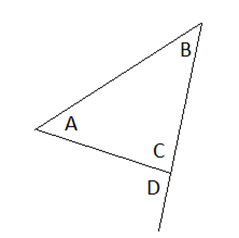
\includegraphics{12}}

All of the following are true EXCEPT

\begin{enumerate}[label=(\Alph*)]
\item $A+B+C=180^\circ$
\item $A+B+C=C+D$
\item $A+B=D$
\item $D=90^\circ$
\item $180^\circ-C=D$
\end{enumerate}}

\vfill
\mitemxx{\medium

\begin{center}
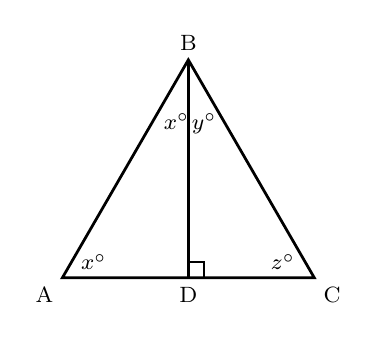
\begin{tikzpicture}
\draw (0,0) node[anchor=north east] {A} -- (4,0) node[anchor=north west] {C} -- (2,3.46) node[anchor=south] {B} -- cycle;
\draw (2,3.46) -- (2,0) node[anchor=north] {D};
\draw (2,0.25) -- (2.25,0.25) -- (2.25,0);
\draw (0.5,0.25) node {$x^\circ$};
\draw (3.5,0.25) node {$z^\circ$};
\draw (2.16,2.75) node[anchor=north east] {$x^\circ$};
\draw (2.25,2.75) node[anchor=north] {$y^\circ$};
\end{tikzpicture}
\end{center}

If $z=30^\circ$, and $BC=3/4$, what is the length of $AC$, rounded to the nearest hundredth?
}{\medium

Triangle $ABC$ has side lengths 6 and 9. Which of the following could be the length of the third side?

\begin{enumerate}[label=\Roman*.]
\item 3
\item 5
\item 15
\end{enumerate}

\begin{enumerate}[label=(\Alph*)]
\item I only
\item II only
\item III only
\item I and II only
\item I, II, and III
\end{enumerate}}

\vfill
\mitemxx{\advanced

A triangle with vertices at points $A (1,4), B(-1,4)$, and $C(7,4)$ is reflected across the $y$-axis. What is the new $y$-coordinate of point $A$?
}{\advanced

What is the largest possible difference in area between two triangles each with side lengths of 7 and 9, rounded to the nearest hundredth?}
\end{multienumerate}

\vfill

\newpage
\subsection{SAT Worksheet 5A (Basic): 6 Questions, 8 Minutes}

\begin{multienumerate}
\mitemxx{A line contains two points with coordinates $(-2,-3)$ and $(7,10)$. Which of the following points are also on the line?

\begin{enumerate}[label=(\Alph*)]
\item $(4,2)$
\item $(9,12)$
\item $(6,5)$
\item $(5,-6)$
\item $(16,23)$
\end{enumerate}
}{A right triangle has a hypotenuse of length 26 and one leg of length 24. What is 200\% of the length of the other leg?

\begin{enumerate}[label=(\Alph*)]
\item 5
\item 10
\item 12
\item 20
\item 24
\end{enumerate}
}

\vfill
\mitemxx{

\medskip
\centerline{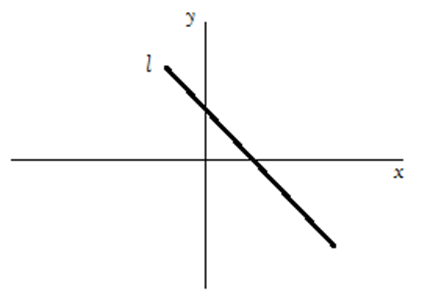
\includegraphics{14}}

Line $l$ has a slope of $-2$ and a $y$-intercept of 2. What is the $x$-intercept of line $l$?

\begin{enumerate}[label=(\Alph*)]
\item $-1$
\item 2
\item 1
\item 4
\item $-2$
\end{enumerate}
}{Points $P, Q$, and $R$ are collinear and graphed on the $xy$ coordinate plane. $R$ is the midpoint of points $P$ and $Q$. $PS$ is the same length as $PR$. Which of the following are plausible?

\begin{enumerate}[label=\Roman*.]
\item Point $S$ has the same coordinates as point $P$
\item $PQ$ is perpendicular to $RS$
\item $PS>PQ$
\end{enumerate}

\begin{enumerate}[label=(\Alph*)]
\item I only
\item II only
\item I and II only
\item I, II, and III
\item None of the above
\end{enumerate}
}

\vfill
\mitemxx{If square $ABCD$ has an area of 5, what is the length of diagonal $AC$?

\begin{enumerate}[label=(\Alph*)]
\item 5
\item $5\sqrt2$
\item 10
\item $10\sqrt2$
\item $\sqrt10$
\end{enumerate}}
{Which of the following equations of lines has a positive slope and has a possible solution of $(3,5)$?

\begin{enumerate}[label=(\Alph*)]
\item $y+3x=5$
\item $-2x+y= -1$
\item $y=2x-10$
\item $x^2-6=y$
\item $2(x+y)=5$
\end{enumerate}}
\end{multienumerate}

\newpage
\subsection{SAT Worksheet 6A (Medium): 6 Questions, 9 Minutes}

\begin{multienumerate}
\mitemxx{

A scalene triangle has side lengths that are each an integer. If the hypotenuse of the triangle is 5, what is the largest possible absolute value difference between the shortest leg and longest leg to the nearest hundredth?

\begin{enumerate}[label=(\Alph*)]
\item 3.00
\item 4.00
\item 1.00
\item 10.00
\item $\sqrt10$
\end{enumerate}
}{

\smallskip
\centerline{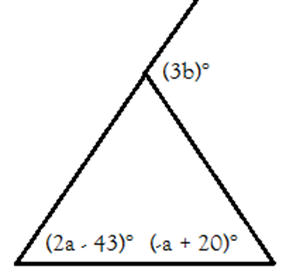
\includegraphics{15}}

\begin{center}
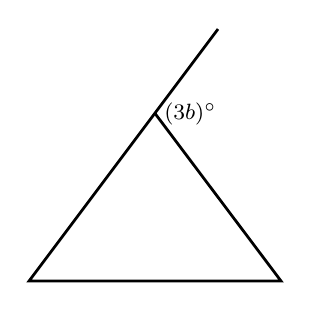
\begin{tikzpicture}
\draw (3,4) -- (0,0) -- (4,0) -- (2,2.66) node[anchor=west] {$(3b)^\circ$};
\end{tikzpicture}
\end{center}

Which of the following expressions can be demonstrated by the figure above?

\begin{enumerate}[label=(\Alph*)]
\item $(a-23)^\circ=3b$
\item $(2a-43)^\circ+(-a+20)^\circ>(3b)^\circ$
\item $(2a-43)^\circ=(-a+20)^\circ$
\item $a=(3b)^\circ20$
\item $a-23>(3b)^\circ$
\end{enumerate}
}

\vfill
\mitemxx{In the $xy$-plane, the points with coordinates $(0,1)$ and $(4,t)$ lie on line $l$. If the slope of l is greater than $1/4$ but less than $1/2$, what is one possible value of $t$?

\begin{enumerate}[label=(\Alph*)]
\item 0
\item 1
\item 1.5
\item 2
\item 2.5
\end{enumerate}
}{On a $xy$-plane, line $l$ is perpendicular to the $x$-axis and is 3 units from the $y$-axis. Which of the following points could be on line $l$?

\begin{enumerate}[label=(\Alph*)]
\item $(1,3)$
\item $(3,5)$
\item $(0,3)$
\item $(2,1)$
\item $(1,2)$
\end{enumerate}}

\vfill
\mitemxx{If a circle has an area of $h\pi$, what is the diameter of the circle?

\begin{enumerate}[label=(\Alph*)]
\item $(2h)^2$
\item $h$
\item $2\sqrt h$
\item $h^2$
\item $\sqrt{h}/2$
\end{enumerate}}
{A circle and a triangle are coplanar. What are the maximum number of intersection points between the two shapes?

\begin{enumerate}[label=(\Alph*)]
\item 3
\item 4
\item 5
\item 6
\item More than 6
\end{enumerate}}
\end{multienumerate}

\newpage
\subsection{SAT Worksheet 7A (Advanced): 6 Questions, 10 Minutes}

\begin{multienumerate}
\mitemxx{The equation $tx+12y=-3$ is the equation of a line in the $xy$-plane, and t is a constant. If the slope of the line is $-10$, what is the value of $t$?}{On an $xy$-plane, Point R has coordinates $(0,r)$ and Point $S$ has coordinates $(s,0)$. What is the slope of line $l$?

\begin{enumerate}[label=(\Alph*)]
\item $-r/s$
\item $r/s$
\item $-s/r$
\item $s/r$
\item $-1/rs$
\end{enumerate}}

\vfill
\mitemxx{Point $A$ has coordinates $(a,b)$ and is in the fourth quadrant. Point $B$ is in the third quadrant. Points $A$ and $B$ are the same distant from the origin. Which of the following could be the coordinates of point $B$?

\begin{enumerate}[label=(\Alph*)]
\item $(-a,b)$
\item $(a,b)$
\item $(-b,-a)$
\item $(-b,a)$
\item $(b,a)$
\end{enumerate}}
{Points on the line $2x+y=1$ lie in which of the following sets of quadrants?

\begin{enumerate}[label=(\Alph*)]
\item I and III only
\item I and IV only
\item I, II, and III
\item I, II and IV
\item I, III, and IV
\end{enumerate}}

\vfill
\mitemxx{In the quadrilateral $ABCD$, point $E$ is on the line segment $AB$. The ratio of $AE$ to $EB$ is $5:4$. $AE=BC=2$. What is the area of the triangle $EBC$?}
{If a cube has an edge of 3, what is the maximum distance from one vertex to another, rounded to the nearest hundredth?}
\end{multienumerate}

\vfill
\pagebreak
\chapter{Geometry Part II}

\subsection{SAT Worksheet 1B: Warm-Up Problems}

\textbf{Strategies Practice:} Read the question, then make a box around what you are trying to solve for. This may be different than what you are solving for, so it is a good check.

\begin{multienumerate}
\mitemxx{\basic

In square $ABCD$, $\angle A$ is $(1/3)x$. What is $(5/3)x$ equal to?

\begin{enumerate}[label=(\Alph*)]
\item $90^\circ$
\item $360^\circ$
\item $180^\circ$
\item $270^\circ$
\item $450^\circ$
\end{enumerate}
}{\medium

What is the measure, in degrees, of the largest of 3 angles that together form a straight line if the ratio of the angles is $5:4:1$?

\begin{enumerate}[label=(\Alph*)]
\item $18^\circ$
\item $72^\circ$
\item $80^\circ$
\item $90^\circ$
\item $180^\circ$
\end{enumerate}}
\end{multienumerate}

\hrulefill

\textbf{Content Practice:} Do the following problems.

\begin{multienumerate}
\mitemxx{\basic

In the $xy$-plane, the line with equation $y=4/5x+3$ intersects the $x$-axis at point $A$ and the $y$-axis at point $B$. What is the length of a line segment from point $A$ to point $B$ rounded to the nearest tenth?}
{\medium
If it is 4:00pm, what is the measure of the angle between the minute and hour hands of the clock?

\begin{enumerate}[label=(\Alph*)]
\item $30^\circ$
\item $90^\circ$
\item $120^\circ$
\item $160^\circ$
\item $180^\circ$
\end{enumerate}}

\mitemx{\advanced

Line $l$ has the equation $y=-6x+5$. What is the equation of line $l$ reflected over the $x$-axis?

\begin{enumerate}[label=(\Alph*)]
\item $-1/6x+5$
\item $6x+5$
\item $-1/6x-5$
\item $1/6x+5$
\item $6x-5$
\end{enumerate}
}
\end{multienumerate}

\newpage
\section{Circles}

Examples:

\begin{multienumerate}
\mitemxx{\basic

In an $xy$-plane, one endpoint of a diameter of a circle is $(-5,-6)$ and the other endpoint of the diamtere is $(7,-6)$. What is the center of the circle?

\begin{enumerate}[label=(\Alph*)]
\item $(0,0)$
\item $(12,-6)$
\item $(1,-6)$
\item $(1,6)$
\item $(12,-12)$
\end{enumerate}}{\medium

The diameter of circle $A$ is 4 times the diameter of circle $B$. What is the ratio of the area of circle $A$ to the area of circle $B$?

\begin{enumerate}[label=(\Alph*)]
\item 2
\item 4
\item 8
\item 12
\item 16
\end{enumerate}}
\end{multienumerate}

\bigskip
Review Questions:

\begin{enumerate}
\item What is the relationship between radius and diameter?
\vfill\item What is the formula for the circumference of a circle? For the circumference of a semicircle?
\vfill\item What is the formula for the area of a circle? Fro the area of a semicircle?
\vfill\item Many SAT problems with circles will give you the area of a circle and ask you to find the circumference of it OR give you the circumference of the circle and ask you to find the circle's area? Conceptually, how would you do either of these scenarios?
\end{enumerate}

\vfill
\newpage
\textbf{New Material}

\bigskip
What is a sector?

\hfill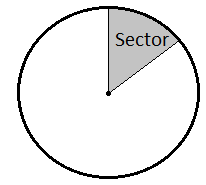
\includegraphics{16}

How can we compare the features of a sector (e.g. area) to the features of a circle and solve for the unknown features?

\vfill
What is the mathematical expression that will allow us to compare the features and solve for the unknown features?

\vfill
Demonstrate your knowledge of the concept by solving the problem below:

\bigskip
The area of circle $A$ (shown to the right) is $25\pi$ cm$^2$. If the area of sector $ABC$ is $10\pi$ cm$^2$, what is the length of arc $BC$?

\hfill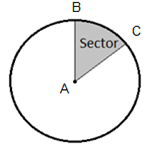
\includegraphics{17}

\newpage
\subsection{SAT Worksheet 2B: 6 Questions, 8 Minutes}

\begin{multienumerate}
\mitemxx{\basic

\centerline{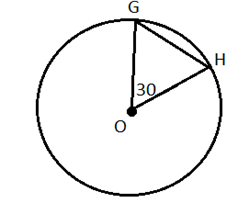
\includegraphics{18}}

\centerline{Note: Figure not drawn to scale}

\bigskip
In the figure above, point $O$ is the center of the circle and $\angle GOH = 30^\circ$. Given that each triangle must have one vertex touching $O$ and the triangles can not overlap, how many triangles identical to $GOH$ could be fit in circle $O$?

\begin{enumerate}[label=(\Alph*)]
\item 5
\item 6
\item 12
\item 24
\item 36
\end{enumerate}}{\basic

Three semicircles with radius 3 are placed on a rectangular sheet of paper with length 10 and width 15. None of the semicircles overlap and they are all completely on the paper. What is the area of the paper not covered by semicircles?

\begin{enumerate}[label=(\Alph*)]
\item $150-(27/2)\pi$
\item $150-(150/2)\pi$
\item $150-(9/2)\pi$
\item $150-(35/2)\pi$
\item $9/2\pi$
\end{enumerate}}

\vfill
\mitemxx{\medium

Joe cut 2 circular pizzas into identical wedge-shaped pieces. The tip of each piece is always at the center of the pizza and the angle at the tip is always greater than $30^\circ$ but smaller than $40^\circ$. Name one possible value for the number of total pieces into which the two pizzas are cut.
}{\medium

A circle has its center at $(2,3)$ and a radius of 4. Which of the following are $x$-coordinates on the circle that have the same $y$-coordinates?

\begin{enumerate}[label=(\Alph*)]
\item $(-1,5)$
\item $(2,3)$
\item $(6,0)$
\item $(-3,7)$
\item $(-2,3)$
\end{enumerate}}

\vfill
\mitemxx{\advanced

\centerline{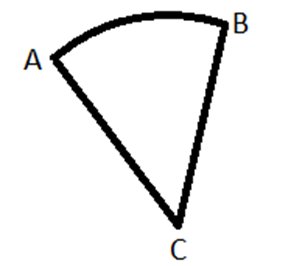
\includegraphics{19}}

In the figure above, $AB$ is the arc of a circle with center $C$. $\angle ACB$ is $40^\circ$. If the area of the circle C is $25\pi$, what is the length of arc $AB$?

\begin{enumerate}[label=(\Alph*)]
\item $2.5\pi$
\item $4.0\pi$
\item $(6/5)\pi$
\item $(10/9)\pi$
\item $1.3\pi$
\end{enumerate}
}{\advanced

\centerline{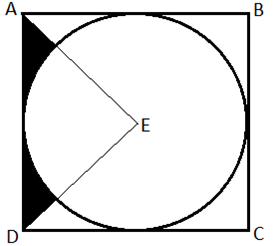
\includegraphics{20}}

In the figure above, square $ABCD$ has an edge of 6. What is the area of the shaded region?

\begin{enumerate}[label=(\Alph*)]
\item $9-(9/4)\pi$
\item $36-9\pi$
\item $36-(9/4)\pi$
\item $36-(9/16)\pi$
\item $9-(9/16)\pi$
\end{enumerate}}
\end{multienumerate}

\newpage
\section{Unusual and Multiple Figures}

Examples:

\begin{multienumerate}
\mitemxx{\medium

A cylinder with height $h$ and radius $e$ is stacked on top of a cube with an edge $e$. What is the ratio of the cylinder volume to the cube volume in terms of $h$ and $e$ in its most simplified form?

\begin{enumerate}[label=(\Alph*)]
\item $e^2h\pi$
\item $(e^2h/e^3)\pi$
\item $(h/e)\pi$
\item $e^{-2}h\pi$
\item $(e/h)\pi$
\end{enumerate}
}{\medium

\centerline{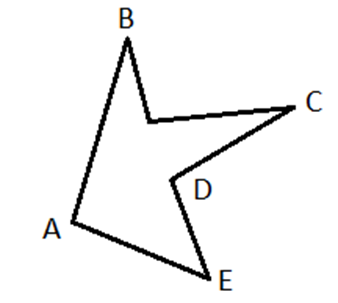
\includegraphics{21}}

In the figure above, the area is 39 square units and the perimeter is four less than two thirds of the area. If the ratio of $AB:BC:CD:DE:AE=3:1:2:2:1:2$, then what is the length of $AB$?

\begin{enumerate}[label=(\Alph*)]
\item 3
\item 4
\item 6
\item 9
\item 12
\end{enumerate}}
\end{multienumerate}

\hrulefill

Strategy for Unusual or Multiple Figures

\begin{enumerate}
\item
\item
\item
\item
\end{enumerate}

\pagebreak
\subsection{SAT Worksheet 3B: 6 Questions, 8 Minutes}

\begin{multienumerate}
\mitemxx{\basic

A plot of land has a perimeter of 48 square meters. What is the largest possible area for this plot of land, in square meters?

\begin{enumerate}[label=(\Alph*)]
\item 36
\item 48
\item 128
\item 144
\item 216
\end{enumerate}
}{\basic

Shape A consists of 22 identically shaped, small squares and has a perimeter of 24 meters and an area of 12 square meters. Shape B consists of 11 identically shaped, small squares that are the same size as the squares in Shape A and a perimeter of 15 meters. What is the area of Shape B, in square meters?

\begin{enumerate}[label=(\Alph*)]
\item 6
\item 7.5
\item 10
\item 11
\item 22
\end{enumerate}}

\vfill
\mitemxx{\medium

\centerline{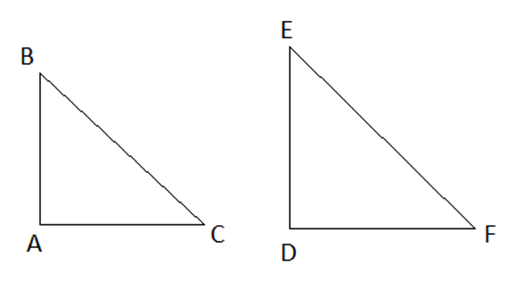
\includegraphics{22}}

Note: Figures are not drawn to scale

\bigskip
Triangles $ABC$ and $DEF$ are similar with a ratio of $5:6$. If $BA=10$, $\angle A$ is $90^\circ$ and $\angle B$ is $45^\circ$, what is the perimeter of triangle $DEF$?

\begin{enumerate}[label=(\Alph*)]
\item $20+10\sqrt2$
\item 30
\item $20+12\sqrt{2}$
\item $24+12\sqrt{2}$
\item 36
\end{enumerate}}
{\medium

\centerline{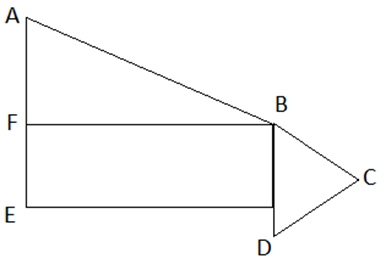
\includegraphics[scale=0.8]{23}}

Note: Figure is not drawn to scale

\bigskip
In the figure above, $BF\perp AF$ and $AF=FE=3$. $BD$ is twice as long as $AF$. If $\angle A=\angle C=\angle D=60^\circ$, what is the perimeter of the figure $ABCDEF$? (Note: The answer should include the perimeter of the unmarked vertex (where $BD$ and $E$ intersect), not just a straight line from $D$ to $E$.)

\begin{multicols}{2}
\begin{enumerate}[label=(\Alph*)]
\item $24+3\sqrt3$
\item 24
\item $20+3\sqrt2$
\item $20+3\sqrt3$
\item $20-3\sqrt3$
\end{enumerate}
\end{multicols}}

\vfill
\mitemxx{\advanced

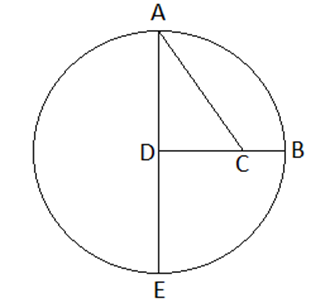
\includegraphics{24}

Note: Figure is not drawn to scale

\bigskip
In the figure above, circle $D$ has a circumference of $16\pi$ meters. If $BC=2$, what is the length of $AC$?

\begin{enumerate}[label=(\Alph*)]
\item 8
\item 10
\item 12
\item 16
\item $8\pi$
\end{enumerate}
}{\advanced

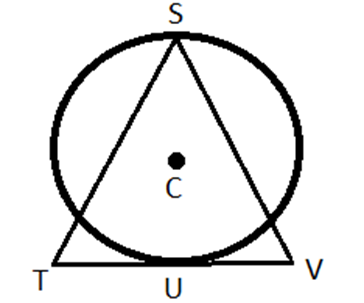
\includegraphics{25}

In the figure above, $SVT$ is an equilateral triangle and $TU=UV$. If the area of the circle is $9\pi$, what is the length of $ST$?

\begin{enumerate}[label=(\Alph*)]
\item $\sqrt{48}$
\item $\sqrt{40}$
\item $\sqrt{51}$
\item $\sqrt{45}$
\item $2\sqrt{11}$
\end{enumerate}}
\end{multienumerate}

\newpage
\section{Volume and Surface Area}

Examples:

\begin{multienumerate}
\mitemxx{\basic

9 small cubes with length 1 are combined to make one large shape. What is the minimum surface area of this larger shape?}
{\medium

The dimensions of an empty rectangular box $A$ are 8 inches by 8 inches by 5 inches. Box $B$ is a solid rectangular box with dimensions 4 inches by 4 inches by $1/3$ inches. What is the maximum number of boxes with the shape of box $B$ that could fit completely into Box $A$?

\begin{enumerate}[label=(\Alph*)]
\item 16
\item 24
\item 60
\item 90
\item 96
\end{enumerate}}
\end{multienumerate}

\hrulefill

\bigskip
Volume - volume is the area of the 2D figure and then multiply it by the height. For example, the volume of a cylinder is the area of a \longline multiplied by the \longline.

\vfill
Surface area - find the area of each side and then take the sum.

\begin{itemize}
\item Draw a cube and then write the formula for the surface area of a cube
\vfill\item Draw a rectangular prism and then write the formula for the surface area of a prism
\vfill\item Draw a cylinder and then write the formula for the surface area of a cylinder
\end{itemize}

\vfill
\pagebreak
\subsection{SAT Worksheet 4B: 6 Questions, 8 Minutes}

\begin{multienumerate}
\mitemxx{\basic

A sphere with a diameter $d$ is inscribed in a cube so that a total of 6 points on the sphere touch the cube. What is the area of the cube?

\begin{enumerate}[label=(\Alph*)]
\item $d^2$
\item $d^3$
\item $(1/8)d^3$
\item $6d$
\item $6d^3$
\end{enumerate}
}{\basic

A rectangular prism has a length of 6 square inches, a width of 6 square inches, and a height of 3 square inches. What is the minimum number of  square feet of wrapping paper would it take to wrap the entire shape?

\begin{enumerate}[label=(\Alph*)]
\item 0.333
\item 0.375
\item 1.0
\item 1.25
\item 108
\end{enumerate}}

\vfill
\mitemxx{\medium

\centerline{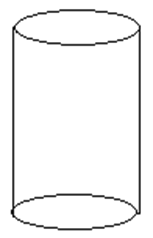
\includegraphics{26}}

Three tennis balls each with a diameter of 4 are placed in a canister of diameter 4 and height 12. Given that the area of a sphere is $4/3\pi r^3$, what is the remaining volume inside of the canister?

\begin{enumerate}[label=(\Alph*)]
\item $48\pi-(16/3)\pi$
\item $48\pi$
\item $24\pi-(8/3)\pi$
\item $24\pi-(16/3)\pi$
\item $48\pi-(112/3)\pi$
\end{enumerate}}{\medium

A rectangular prism with length 3, width 4, and height 7 has volume $v$. What is the volume of a rectangular prism with length 6, width 7, and height 1 in terms of $v$?

\begin{enumerate}[label=(\Alph*)]
\item $v$
\item $2v$
\item $v/4$
\item $42$
\item $v/2$
\end{enumerate}}

\vfill
\mitemxx{\advanced

A cylindrical water tank of height 10 square feet and a diameter of 10 square feet is filled with $\pi$ square inches of water every minute. How long would it take to fill 75\% of the water tank, in minutes?

\begin{enumerate}[label=(\Alph*)]
\item $75$
\item $62.5\pi$
\item $250/3$
\item $187.5$
\item $250\pi$
\end{enumerate}}{\advanced

A rectangular cylinder has a radius of $s$ and height $s$. What is the volume of the smallest cube that could be used to enclose this cylinder, in terms of $s$?

\begin{enumerate}[label=(\Alph*)]
\item $s^3/8$
\item $2s^3$
\item $s^3$
\item $8s^3$
\item $s^2$
\end{enumerate}}
\end{multienumerate}

\pagebreak
\subsection{SAT Worksheet 5B (Basic): 6 Questions, 8 Minutes}

\begin{multienumerate}
\mitemxx{1.  The area of square $A$ is $n$ and square $B$ has a side length that is twice that of square $A$. Which expression represents the area of square $B$?

\begin{enumerate}[label=(\Alph*)]
\item $n$
\item $n^2$
\item $n^4$
\item $2n$
\item $4n$
\end{enumerate}}{For which given value for the radius of a circle is the area greater in value than the circumference?

\begin{enumerate}[label=(\Alph*)]
\item 0.5
\item 1
\item 1.5
\item 2
\item 2.5
\end{enumerate}}

\vfill
\mitemxx{

\centerline{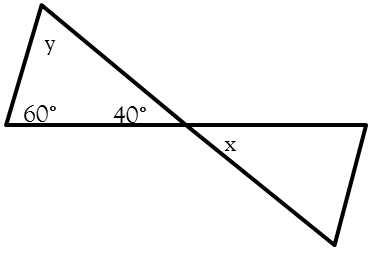
\includegraphics{27}}

In the figure above, what is the value of $x+y$?

\begin{enumerate}[label=(\Alph*)]
\item $70^\circ$
\item $80^\circ$
\item $100^\circ$
\item $120^\circ$
\item $140^\circ$
\end{enumerate}}{

\centerline{
\includegraphics{28}}

In the figure above, the area of the inner most concentric circle is $9\pi$ cm. If each subsequent circle increases in radius by 1, what is the area of the outermost circle?

\begin{enumerate}[label=(\Alph*)]
\item $25\pi$
\item $36\pi$
\item $49\pi$
\item $121\pi$
\item $169\pi$
\end{enumerate}}

\vfill
\mitemxx{The total sum of the interior angles of a regular pentagon is $6m$. What is the measure of one angle?

\begin{enumerate}[label=(\Alph*)]
\item $m$
\item $5m$
\item $6m$
\item $(5/6)m$
\item $(6/5)m$
\end{enumerate}}{If the length of the diagonal of a square doubles, what ratio is the original side length to the new one?

\begin{enumerate}[label=(\Alph*)]
\item $1:2$
\item $1:4$
\item $2:1$
\item $4:1$
\item $1:\sqrt{2}$
\end{enumerate}}
\end{multienumerate}

\newpage
\textbf{\large SAT Worksheet 6B (Medium): 6 Questions, 9 Minutes}

\begin{multienumerate}
\mitemxx{

\medskip
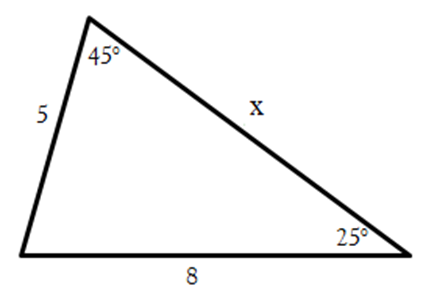
\includegraphics{29}

Which of the following could be a possible value of $x$ in the figure above?

\begin{enumerate}[label=(\Alph*)]
\item 3
\item 6
\item 7
\item 11
\item 13
\end{enumerate}}{

\medskip
\centerline{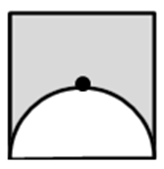
\includegraphics{30}}

Determine the area of the shaded region to the nearest hundredth in the figure above if the radius of the circle is 3.}

\vfill
\mitemxx{A 13 ft. ladder is propped against a building. If the top of the ladder reaches a height of 12 ft. on the building, what is the distance of base of the ladder to the base of the building in feet?

\begin{enumerate}[label=(\Alph*)]
\item 4
\item 5
\item 8
\item 11
\item 12
\end{enumerate}}{4. The surface area of a cube is equal to its volume. What is the length of the sides?

\begin{enumerate}[label=(\Alph*)]
\item 2 units
\item 4 units
\item 6 units
\item 8 units
\item 16 units
\end{enumerate}}

\vfill
\mitemxx{Find the measure of the radius of a right cylinder whose volume is twice the value of the height to the nearest hundredth.}{The volume of a ball is given by kπ where k is a positive integer. Which of the following is the smallest possible value of the volume? (The volume of a sphere is $4/3\pi r^3$.)

\begin{multicols}{2}
\begin{enumerate}[label=(\Alph*)]
\item $9\pi$
\item $12\pi$
\item $16\pi$
\item $36\pi$
\item $54\pi$
\end{enumerate}
\end{multicols}}
\end{multienumerate}

\pagebreak
\subsection{SAT Worksheet 7B (Advanced): 6 Questions, 10 Minutes}

\begin{multienumerate}
\mitemxx{If the area of an equilateral triangle is doubled, what is the ratio of the old side length to the new one?

\begin{enumerate}[label=(\Alph*)]
\item $1:\sqrt{2}$
\item $1:\sqrt{3}$
\item $1:2$
\item $1:3$
\item $2:\sqrt{3}$
\end{enumerate}}{In the figure below, the area of the inner circle is $6\pi$ and each outer circle has a width of 1 cm. greater than the previous circle. Determine the ratio of the radius of the outermost circle to the inner most.

\centerline{
\includegraphics{31}}

\begin{enumerate}[label=(\Alph*)]
\item $6+4\sqrt{6}:6$
\item $6+2\sqrt{6}:6$
\item $2:3$
\item $3:4$
\item $1:3$
\end{enumerate}}

\vfill
\mitemxx{The area of a rectangle is equal to its perimeter. If the sum of the length and the width is 9, what is the length of the diagonal?

\begin{enumerate}[label=(\Alph*)]
\item $\sqrt{5}$
\item $3\sqrt{5}$
\item $2\sqrt{5}$
\item $3\sqrt{2}$
\item $5\sqrt{2}$
\end{enumerate}}{A cube with an edge of 3 cm. consists of smaller $1\times1$ cm. cubes. If the outer faces of the cube were painted, what is the ratio of the outer faces to the total number of faces of each smaller cube?

\begin{enumerate}[label=(\Alph*)]
\item $1:3$
\item $1:6$
\item $1:2$
\item $2:3$
\item $1:4$
\end{enumerate}}

\vfill
\mitemxx{

\medskip
\centerline{
\includegraphics{32}}

A picture has a frame of uniform width. The dimensions of the frame are 12 cm and 8 cm. If the area of the picture is 32 cm$^2$, which of the following must be the width of the frame?

\begin{enumerate}[label=(\Alph*)]
\item 2 cm
\item 3 cm
\item 4 cm
\item 5 cm
\item 6 cm
\end{enumerate}}{

\medskip
\centerline{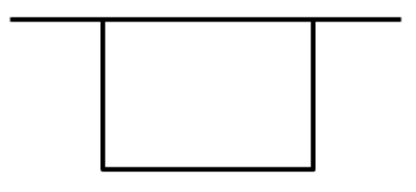
\includegraphics{33}}

Brandy wants to build a small fence around her rectangular garden that is adjacent to a wall. If she buys 40 feet of fencing, what is the maximum area of the garden she can cover?

\begin{enumerate}[label=(\Alph*)]
\item 10 ft$^2$
\item 24 ft$^2$
\item 100 ft$^2$
\item 200 ft$^2$
\item 400 ft$^2$
\end{enumerate}}
\end{multienumerate}
\chapter{Geometry Part III}

\subsection{Worksheet 1C: Warm-Up Problems}

\textbf{Strategies Practice:} The SATs will test the same concept(s) in many different ways. Identify what area(s) the questions use. If you need help, then you can refer to the “About the math section at the beginning of this guide. Then, solve the questions.

\begin{multienumerate}
\mitemxx{\medium

Lauren and Rebecca leave Dave's house at the same time. Lauren walks east for an average at 6 miles per hour and continues for 3 hours. Rebecca scooters south for an average at 8 miles per hour for 3 hours. At the end of these 3 hours, what is the straight-line distance between them, in miles?

\begin{enumerate}[label=(\Alph*)]
\item 10
\item 18
\item 24
\item 30
\item 36
\end{enumerate}
}{\advanced

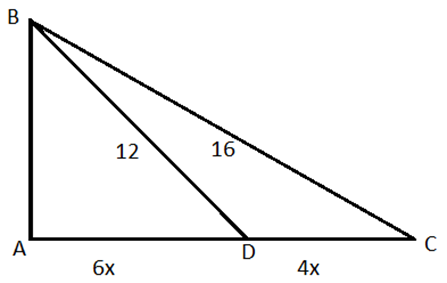
\includegraphics{34}

$\angle DAB$ is $90^\circ$. What is the length of $BA$?}
\end{multienumerate}

\vfill
\pagebreak
\section{Geometric Probability}

\begin{multienumerate}
\mitemxx{\basic

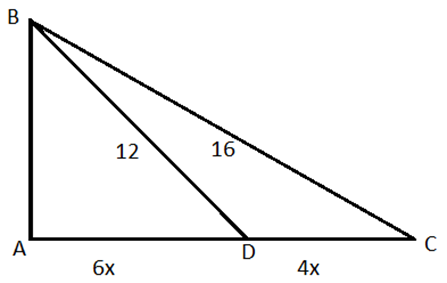
\includegraphics{34}

Note: Figure is not drawn to scale

\bigskip
In the figure above,$ B, D, F$, and $H$ are midpoints of $AC, CE, EG$, and $GA$, respectively. If a marble is thrown randomly and lands in rectangle $ACEG$, what is the probability that it lands on the shaded region?

\begin{enumerate}[label=(\Alph*)]
\item 1/4
\item 2/3
\item 1/2
\item 3/4
\item 4/5
\end{enumerate}
}{\medium

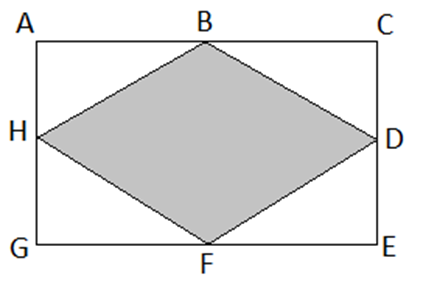
\includegraphics{35}

Three circles with the same center but different radii are combined to make the circular dartboard in the figure above. The circle enclosing the 1 point region has a radius that is two times bigger than the 3 point region and three times bigger than the 5 point region. If a dart thrown at random lands on the board, what is the probability that the person will get 3 points?

\begin{enumerate}[label=(\Alph*)]
\item 1/4
\item 2/11
\item 1/5
\item 1/3
\item 3/13
\end{enumerate}}
\end{multienumerate}

\hrulefill

\bigskip
Geometric probability uses probability concepts (the chance of an event occurring) to analyze shapes (which you use to find the chance of all possible events occurring).

\bigskip
The general formula is:

\vfill
\pagebreak
\subsection{SAT Worksheet 2C: 6 Questions, 8 Minutes}

\begin{multienumerate}
\mitemxx{\basic
\centerline{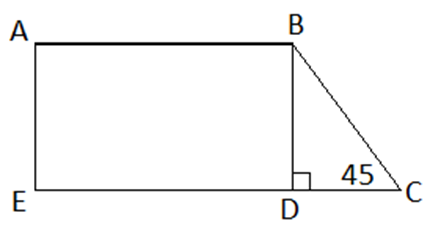
\includegraphics{37}}

In the figure $ABCDE$ above, $(1/2)AB=BD=5$ and $\angle C=45^\circ$. If a marble is rolled randomly and lands on the figure $ABCDE$, what is the probability that it lands on triangle $BCD$?

\begin{enumerate}[label=(\Alph*)]
\item 1/12
\item 1/10
\item 1/6
\item 1/5
\item 1/4
\end{enumerate}}{\basic

\centerline{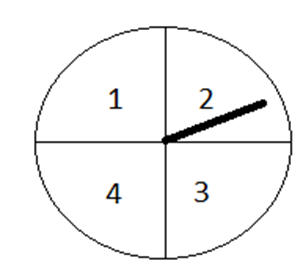
\includegraphics{38}}

If the circular spinner above was changed to have 6 identical sectors instead of 4, what is the probability of spinning twice and each time getting a number greater than 3?

\begin{enumerate}[label=(\Alph*)]
\item 1/4
\item 1/3
\item 1/6
\item 1/2
\item 2/3
\end{enumerate}}

\vfill
\mitemxx{\medium

\centerline{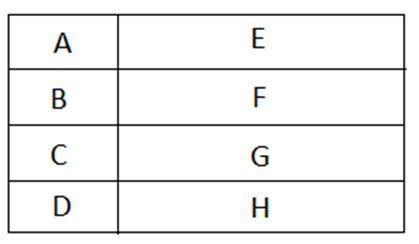
\includegraphics{39}}

In the figure above, boxes $A, B, C$, and $D$ are congruent. Box $E$ is 4 times bigger than box $A$ and is congruent to boxes $F, G$, and $H$. Two darts are thrown at the figure at random and lands on two of the boxes. What is the probability that Box E is hit both times?
}{\medium

\centerline{
\includegraphics{40}}

\centerline{Note: Figure is not drawn to scale}

\bigskip
If the black ring has a diameter of 6 and the white ring inside the larger circle has a diameter of 4, what is the ratio of area of the black ring to the white ring?

\begin{enumerate}[label=(\Alph*)]
\item $9:4$
\item $3:2$
\item $5:1$
\item $11:3$
\item $6:1$
\end{enumerate}}

\vfill
\mitemxx{\advanced

\centerline{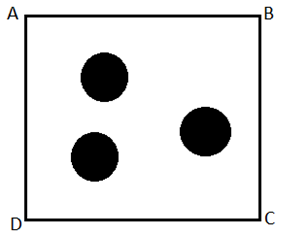
\includegraphics{41}}

The figure above shows the top view of an open square box that has an edge of length $l$. Each of the 3 circles have a diameter of length $l/2$. When a marble is into the box at random, it falls on either the circles or the background. What is the probability that the marble will not fall in one of the circles?

\begin{enumerate}[label=(\Alph*)]
\item $1-(3\pi/16)l$
\item $1-(1/4)l$
\item $(1/4)\pi l$
\item $1-\pi/16$
\item $1-(3/4)\pi l$
\end{enumerate}}{\advanced

An artist paints one side of a rectangular piece of cardboard 3 different colors, red, green, and blue. First, he paints 1/5 of the cardboard red. Then, he paints the remaining piece of cardboard equal parts red, green, and blue (none of the colors overlap). If a marble is rolled randomly on the cardboard, what is the probability that it will land on a space that is red rounded to the nearest hundredth?}
\end{multienumerate}

\vfill
\pagebreak
\section{Geometry Mixed Review}

\textbf{Strategy Recap}

\begin{itemize}
\item Strategy \#1: Draw a diagram. If one is already provided, then label the diagram.

\bigskip
\hrulefill

When a line represented by the expression $y+2x+5=0$ is plotted on a $xy$-coordinate graph, the line passes through which quadrants on the $xy$-coordinate graph?

\begin{enumerate}[label=(\Alph*)]
\item I only
\item I and III only
\item II only
\item I, II, and III only
\item I, II, III, and IV
\end{enumerate}

\hrulefill

\bigskip
\item Strategy \#2: Recognize what topic(s) the question is testing. Remember that the more difficult problems on the test will often combine two medium level topics.

\bigskip
\hrulefill

\begin{multicols}{2}
a) In the figure on the left, lines $l$ and $k$ are parallel. If $a=-3$, what is the value of $b^\circ$?

\vfill
b) What math content areas are used to solve this problem?

\vfill

\columnbreak
\centerline{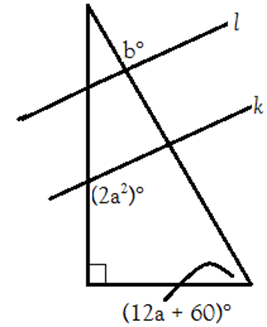
\includegraphics{42}}
\end{multicols}
\hrulefill

\bigskip
\item Strategy \#3: After you solve for your answer, make sure that what you selected matches what the question is asking for. This is critical in problems that require solving for variables.

\bigskip
\hrulefill

The diagonal of rectangle $ABCD$ is $2\sqrt{5}$ and the length of the rectangle is twice its width. What is the area of the rectangle?

\vfill
\hrulefill
\end{itemize}

\pagebreak
\subsection{SAT Worksheet 3C (Basic): 6 Questions, 8 Minutes}

\begin{multienumerate}
\mitemxx{If the area of a circle is 6 square inches, what is the perimeter of the circle?

\begin{enumerate}[label=(\Alph*)]
\item $12\pi$
\item $4\pi$
\item $2\sqrt{6}\pi$
\item $6\pi$
\item $\sqrt{6}\pi$
\end{enumerate}}{If the sum of the circumferences of two congruent circles is $40\pi$, what is the radius of one of the circles?

\begin{enumerate}[label=(\Alph*)]
\item 4
\item $4\pi$
\item 8
\item 10
\item 20
\end{enumerate}}

\vfill
\mitemxx{A town is building a water tower and wants to build a tower that can hold the most water. Which of the following designs would hold the most water?

\begin{enumerate}[label=(\Alph*)]
\item Rectangular prism with length and height of 3 and width of 6
\item Cube with length 5
\item Rectangular prism with a base area of 4.5 and height of 10
\item Cylinder with a radius of 2 and height of 4
\item Triangular prism with a base of 4, altitude of 5, and height of 10
\end{enumerate}}{Points $A, B$, and $C$ lie on a circle whose center is $D$ and radius of 5. If the measure of $\angle ADB$ is $45^\circ$, what is the length of arc $AB$?

\begin{enumerate}[label=(\Alph*)]
\item $\pi/2$
\item $1.25\pi$
\item $1.50\pi$
\item $1.75\pi$
\item $2.0\pi$
\end{enumerate}}

\vfill
\mitemxx{

\medskip
\centerline{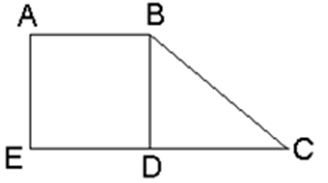
\includegraphics{43}}

One side of square $ABDE$ is 2. Angle C is $45^\circ$. What is integer closest to the perimeter of shape $ABCDE$?}{

\medskip
\centerline{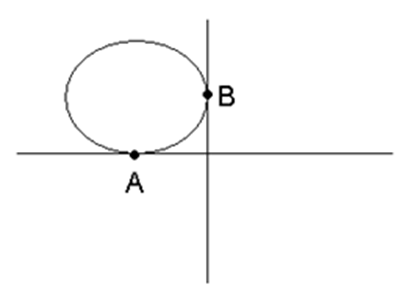
\includegraphics{44}}

The above figure is a circle that is tangent to points $A$ and $B$. If $B$ has coordinates $(0, 3)$, then what is the $x$-coordinate of Point $A$?}
\end{multienumerate}

\vfill
\pagebreak
\subsection{SAT Worksheet 4C (Medium): 6 Questions, 9 Minutes}

\begin{multienumerate}
\mitemxx{Points $A$ and $B$ lie on a circle whose center is $D$. If the area of the sector enclosing $AB$ is $9\pi$ square meters and the area of the full circle is $36\pi$ square meters, what is the measure of the arc length $AB$?

\begin{enumerate}[label=(\Alph*)]
\item $\pi$
\item $2\pi$
\item $3\pi$
\item $5\pi$
\item $9\pi$
\end{enumerate}}{A cube has an edge of $2x$. What is the total surface area of the cube?

\begin{enumerate}[label=(\Alph*)]
\item $24x^2$
\item $12x^2$
\item $10x^2$
\item $8x^2$
\item $8x^3$
\end{enumerate}}

\vfill
\mitemxx{Marlene currently starts at her house and drives 5 miles west, then 12 miles north and then 6 miles west to get to her work. How much longer is this route, in miles, than the number of miles in the route directly from her house to her work, rounded to the nearest hundredth?}
{A vase in the shape of a rectangular prism has height 12 centimeters and a base with an area of 25 square centimeters. When the vase is 3/4 filled with water, what is the volume of the water?}

\vfill
\mitemxx{

\medskip
\centerline{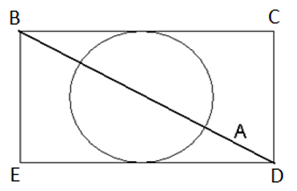
\includegraphics{45}}

A circle is inscribed inside of rectangle $BCDE$ in the figure $BC=8$ and the length of the diagonal, $A$, is 10. What is the radius of the circle?
\begin{enumerate}[label=(\Alph*)]
\item 3
\item 4
\item 8
\item 10
\item Unable to determine based on available information
\end{enumerate}}{The diameter of a circle is 5 inches more than its radius. What is the area of the circle, in square inches?


\begin{enumerate}[label=(\Alph*)]
\item 2.5
\item 5
\item 10
\item $12.25\pi$
\item $25\pi$
\end{enumerate}}
\end{multienumerate}

\pagebreak
\subsection{SAT Worksheet 5C (Advanced): 6 Questions, 10 Minutes}

\begin{multienumerate}
\mitemxx{A rectangular prism has a length of s square inches, a width of $2s$ square inches, and a height of $s$ square inches. What is the minimum number of square feet of wrapping paper in terms of $s$ would it take to wrap the entire shape?

\begin{enumerate}[label=(\Alph*)]
\item $6s^2$
\item $2s^3$
\item $6s^3$
\item $10s^3$
\item $12s^3$
\end{enumerate}}{If the diameter of a circle is doubled, by what percent will the area of the circle increase?

\begin{enumerate}[label=(\Alph*)]
\item $150\%$
\item $200\%$
\item $225\%$
\item $300\%$
\item $400\%$
\end{enumerate}}

\vfill
\mitemxx{A prism has the base of an equilateral triangle with a side length of 6. The height of the triangular prism is 8. What is the volume of the triangular prism?

\begin{enumerate}[label=(\Alph*)]
\item 9
\item 42
\item $72\sqrt{3}$
\item 144
\item $144\sqrt{3}$
\end{enumerate}}{Two cylindrical cans are stacked on top of each other. The height of a right circular cylinder is 6 and the diameter of the base is 10. Which of the following is a possible distance from the center of the base at the bottom to a point on the edge of the other can?

\begin{enumerate}[label=(\Alph*)]
\item 5
\item $\sqrt{61}$ (approximately 7.81)
\item 10
\item 12
\item 1
\end{enumerate}}

\vfill
\mitemxx{

\medskip
\centerline{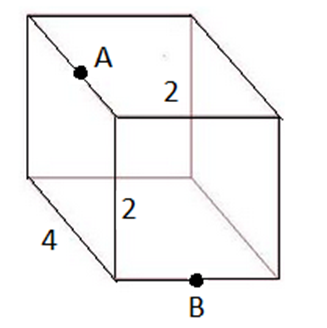
\includegraphics{46}}

The rectangular prism show above has a length and a height of 2, and a width of 4. If points $A$ and $B$ are midpoints of two edges, what is the length of $AB$?

\begin{enumerate}[label=(\Alph*)]
\item 2
\item $2\sqrt{2}$
\item $\sqrt{8}$
\item 3
\item Unable to determine based on available information
\end{enumerate}}{

\medskip
\centerline{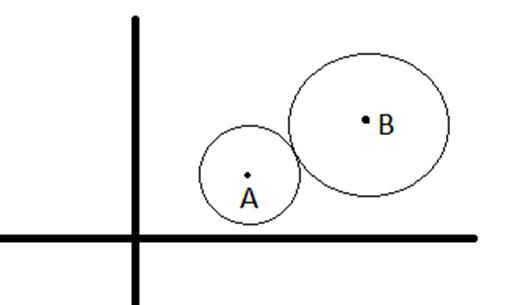
\includegraphics{47}}

In the figure above, there are two circles with centers $A$ and $B$ respectively. Line segment $AB=12$ and center $A$ has the coordinates $(4, 3)$. If the coordinates of center $B$ is $(7, b)$, what is the value of $b$, rounded to the nearest hundredth?}
\end{multienumerate}
\chapter[Problem-Solving Strategies]{Problem-Solving Strategies for SAT Math Sections}

\subsection{Worksheet 1D: Warm-Up Problems}

\bigskip
\textbf{\underline{Algebra and Data Analysis Vocabulary}: Read the words and definitions (if you don't already know them) and then answer the question that follows.}

\begin{enumerate}[label=\bfseries\arabic*.]
\item \textbf{Constant} - A value represented by a variable that will not change

\bigskip
The constant $a$ represents the speed in miles per hour that a car can drive. If said car drives 125 miles in 2.5 hours, what is the value of $a$?

\vfill
\item \textbf{Expression} - A function or any combination of constants. Solve the expression when $x$ is equal to six: $3x+7$

\vfill
\item \textbf{Distributed equally} - Split up in equal parts and given to multiple people

\bigskip
A rectangular pizza measuring 80 cm long and 60 cm wide is cut into square pieces each with an area of 400 cm$^2$ and distributed equally among 4 friends. How many pieces did each person get?

\vfill
\item \textbf{Set of integers, elements} - A set is a group of numbers. The numbers within the set are referred to as elements.

\bigskip
How many elements in the set of the first 8 prime numbers have 3 in their one's digit?

\vfill
\item \textbf{Domain, Range} - The domain is the set of all possible $x$ values. The range represents all possible $y$ values.

\bigskip
What is the domain and range of the following equation $y=|3x+5|$

\vfill
\item \textbf{Average/Arithmetic mean, median, mode} - In a set of numbers the average is the sum of all values divided by the number of values. The median is the middle value. The mode is the most common value.

\bigskip
Find the mean, median, and mode of this set of numbers:

\[10,20,20,40,50,90,120\]

Mean:

\medskip
Median:

\medskip
Mode:
\end{enumerate}

\vfill
\pagebreak
\section[SAT Algebra]{General Strategies for SAT Algebra}

It can be difficult to know every concept on the SATs or more frequently, which topic(s) is best used to solve the problem. Therefore, if you get to a problem that you don't know how to solve, then you can use the following strategies to help you find the right answer. They spell the acronym PUFS (like the tissue company but with only 1 letter ``F'').

\bigskip
\textbf{\large P}lug in real numbers

\medskip
\textbf{\large U}se the answer choices

\medskip
\textbf{\large F}ormulas

\medskip
\textbf{\large S}ee the problem

\hrulefill

\textbf{SAT Math Strategy 1: Plug in real number}

\bigskip
Many SAT problems are made unnecessarily tricky by using \longline instead of \longline.

\begin{enumerate}
\item Assigning each variable a unique, \longline (for example, if there are variables $a, b$, and $c$ in the problem, make $a=2, b=3, c=5$). These numbers should be easy to work with. If you are using percentages, it is recommended to use \longline for the base variable because percentages are out of 100.
\item Solve the problem with these \longline instead of variables.
\item If necessary, translate the numbers back to \longline, percentages, fractions, etc
\end{enumerate}

\textbf{Try It:} If $a$ is 1/3 of $b$ and $b$ is 2/5 of $z$ and $z>0$, then $a$ is what percentage of $z$?

\pagebreak
\subsection{SAT Worksheet 2D: 6 Questions, 8 Minutes}

\begin{multienumerate}
\mitemxx{\basic

Which of the following could be the remainders when 3 consecutive, even, positive integers are each divided by 5?

\begin{enumerate}[label=(\Alph*)]
\item $1,2,3$
\item $1,4,6$
\item $0,1,4$
\item $1,3,0$
\item $2,3,4$
\end{enumerate}}{\basic

If $(1/5)a+b=b^2-a$, what is $a$ in terms of $b$?

\begin{enumerate}[label=(\Alph*)]
\item $b^2-b$
\item $5(b^2-b)$
\item $1/5(b^2-b)$
\item $b-\sqrt{b}$
\item $5/6(b^2-b)$
\end{enumerate}}

\vfill
\mitemxx{\medium

When some integer $b$ is divided by 4, the remainder is 3. How many values of $b$ are between 0 and 40?

\begin{enumerate}[label=(\Alph*)]
\item Five
\item Seven
\item Eight
\item Nine
\item Ten
\end{enumerate}}{\medium

\medskip
\begin{tabular}{|l|c|c|c|}\hline
& Bus & Non-bus & \textbf{Total}\\\hline
9\textsubscript{th} graders & A & B & C\\\hline
10\textsubscript{th} graders & D & E & F\\\hline
11\textsubscript{th} graders & G & H & I\\\hline
\textbf{Total} & J & K & L\\\hline
\end{tabular}

\medskip
The chart above has a letter to represent the number of students in each category. Which of the following equals $A$?

\begin{enumerate}[label=(\Alph*)]
\item $I-(G+E)-B$
\item $F-E+D$
\item $J-(I-H)-D$
\item $H-E-(C-B)$
\item None of the above
\end{enumerate}}

\vfill
\mitemxx{\advanced

If $a$ and $b$ are positive integers and $4^a=2^b/2$, what is $a$ in terms of $b$?

\begin{enumerate}[label=(\Alph*)]
\item $b/2$
\item $b^{1/2}$
\item $b$
\item $(b-1)/2$
\item $2b$
\end{enumerate}}{\advanced

The ratio of fruit juice to water in Betty's orange juice is $7:3$. How many liters of fruit juice is in 2 liters of Betty's orange juice?}
\end{multienumerate}

\pagebreak
\textbf{SAT Math Strategy 2: Use the answer choices}

If the question is multiple choice, then you may be able to plug in the answer choices into the question to see which answer choice gives you the correct answer.

\bigskip
Hint: It is suggested in SAT literature that if you try this approach, that you should start with answer choice C and work outwards or answer choice E and go backwards from E to A because the SATs will rarely make problems that can be solved with this strategy to have answer choice A. 

\bigskip
\textbf{Try It:} What is the smallest of 5 consecutive even integers if the sum of these integers equals 300?

\begin{enumerate}[label=(\Alph*)]
\item 50
\item 52
\item 54
\item 56
\item 58
\end{enumerate}

\newpage
\subsection{SAT Worksheet 3D: 4 Problems, 5 Minutes}

\begin{multienumerate}
\mitemxx{\medium

If $a$ is a positive integer, what is the smallest value of $a$ for which $a^2+1.5a$ is an integer?

\begin{enumerate}[label=(\Alph*)]
\item 1/3
\item 1/2
\item 1
\item 2
\item 3
\end{enumerate}}{\medium

A salesman receives \$500 per week and a 5\% commission on each car he sells. If he sold 18 cars at the same price and earned \$3600 in one month, what is the price of 1 car that he sold? (1 month = 4 weeks)

\begin{enumerate}[label=(\Alph*)]
\item \$1,777.78
\item \$3,444.44
\item \$4,000.00
\item \$32,000.00
\item Cannot be determined from the information given
\end{enumerate}}

\vfill
\mitemxx{\advanced

Function $f$ is defined as $f(t)=t-4$ and function $g$ is defined as $g(t)=t^2-32$. For what value of $t$ does $2f(t)=g(t)$?

\begin{enumerate}[label=(\Alph*)]
\item $-6$
\item $-4$
\item 0
\item 2
\item 4
\end{enumerate}}{\advanced

You are given that $(x+2)(x-b)=x^2+cx-8$ where $b$ and $c$ are constants. What is the value of $1/2c$

\begin{enumerate}[label=(\Alph*)]
\item $-2$
\item $-1$
\item 1
\item 2
\item 8
\end{enumerate}}
\end{multienumerate}

\vfill
\pagebreak
\textbf{SAT Math Strategy \#3: Quickly recall and write down general formulas}

Look at the formulas that are given on the SATs and memorize the ones that aren't. Fill in the formulas below that are not given on the SAT test:

\bigskip
Formula for directly proportional:

\bigskip
Formula for inversely proportional:

\bigskip
Formula for average:

\bigskip
Formula for slope:

\bigskip
Formula for equation of a line:

\bigskip
**When you get to a problem that calls for a topic with a formula associated with it, write the general formula in words on your test booklet. For example, if there was a question that has to do with averages we would write down \longline. Then, rewrite the formula with the numbers or variables from the problems filled in.**

\vfill
\textbf{Try it:} 30\% of the students in Ms. Law's class had an average test score of 78 points. The rest of the class had an average test score of 84 points. What is the average test score for all students in Ms. Law's class?

\begin{enumerate}[label=(\Alph*)]
\item 79.5
\item 81.0
\item 82.2
\item 83.0
\item 83.1
\end{enumerate}

\vfill
\newpage
\subsection{SAT Worksheet 4D: 4 Questions, 5 Minutes}

\begin{multienumerate}
\mitemxx{\basic

If $y$ is directly proportional to $x$ and $y=-7$ when $x=2$, what is the value of $x$ rounded to the closest integer when $y=2$?

\begin{enumerate}[label=(\Alph*)]
\item $-7$
\item $-2$
\item $-1$
\item 0
\item 2
\end{enumerate}}{\basic

If $y$ is inversely proportional to $x$ and $y=-7$ when $x=2$, what is the value of $x$ when $y=5.5$?

\begin{enumerate}[label=(\Alph*)]
\item $-2.55$
\item $-1.57$
\item $-0.61$
\item $-0.27$
\item 1
\end{enumerate}}

\vfill
\mitemxx{\medium

If the average of $2a$ and $1/3a$ is 6, what is the value of $5a$?}{\medium

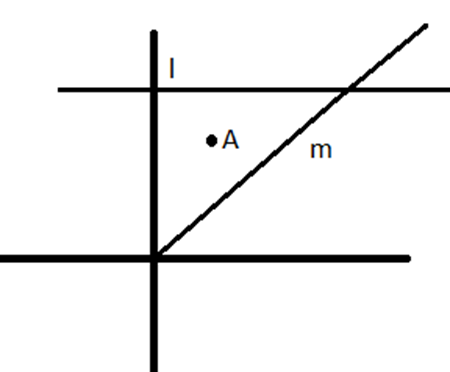
\includegraphics{48}


In the figure above, line $m$ has a slope of 3/4 and the equation of line $l$ is $y=5$. If A is between line $m$ and line $l$ and the $x$-coordinate of point $A$ is 2, how many possible integer values are there for the $y$-coordinate of point $A$?

\begin{enumerate}[label=(\Alph*)]
\item 0
\item 1
\item 2
\item 3
\item More than 3
\end{enumerate}}
\end{multienumerate}

\newpage
\textbf{SAT Math Strategy 4: See and solve the problem using visuals like diagrams, charts, or tables}

\bigskip
Drawing a diagram, table, or chart can help you to visualize the problem, particularly for

\longline and \longline problems. They don't need to be detailed or drawn perfectly-just enough to for you to see the information that you currently have and what you need to solve for.

\bigskip
\textbf{Try It:} 5 students are going to be lined up against a wall. In how many different ways can the 5 students be arranged in a row?

\begin{enumerate}[label=(\Alph*)]
\item 5
\item 24
\item 25
\item 100
\item 120
\end{enumerate}

\newpage
\subsection{SAT Worksheet 5D: 6 Questions, 8 Minutes}

\begin{multienumerate}
\mitemxx{\basic

The ratio of the interior angles in a quadrilateral is $2:5:6:10$. What is the positive difference between the smallest and the largest angle?}{\basic

For example, 3 tennis balls numbered 1-3 and 4 tennis rackets are numbered 1-4, how many different combinations of 1 tennis ball and 1 tennis rackets are possible?

\begin{enumerate}[label=(\Alph*)]
\item 6
\item 7
\item 12
\item 16
\item 24
\end{enumerate}}

\vfill
\mitemxx{\medium

At Jamestown high school, there are 500 students.  20\% of students study biology and 50\% more students study psychology than biology. If 40 students study both biology and psychology, what is the number of Jamestown high school students that do not study biology or psychology?}{\medium

The points $RST$ are colinear and appear in that order. $RT=28$ and $RS=1/3ST$. Point $U$ is then drawn so that it is the midpoint of $RS$ and point $V$ is drawn between  $S$ and $T$ so that $SV=4/5ST$. What is the length of $UV$?   %I clarified the location of SV here

\begin{enumerate}[label=(\Alph*)]
\item 10.5
\item 14.2
\item 17.2
\item 20.3
\item 21
\end{enumerate}}

\vfill
\mitemxx{\advanced

The area of an equilateral triangle $ABC$ is twice the size of the perimeter of equilateral triangle $DEF$. If one side length of $DEF$ is 6 2/3 inches, what is the length of one side in the triangle $ABC$, in inches, rounded to the nearest hundredth?}{\advanced

Abby, Biana, Colin, David, and Ed are going to be lined up against a wall. In how many different ways can the 5 students be arranged in a row if Ed can not be first or last in line?

\begin{enumerate}[label=(\Alph*)]
\item 10
\item 25
\item 72
\item 96
\item 120
\end{enumerate}}
\end{multienumerate}

\newpage
\subsection{SAT Worksheet 6D (Basic): 6 Questions, 8 Minutes}

\begin{multienumerate}
\mitemxx{Which of the following numbers when square rooted, is greater than itself?

\begin{enumerate}[label=(\Alph*)]
\item 1/2
\item 3/4
\item 4/3
\item 5/4
\item 6/5
\end{enumerate}}{If $3x+ky=1$ has a slope of $-2$, what is the value of $k$?

\begin{enumerate}[label=(\Alph*)]
\item $-6$
\item $-3/2$
\item 2/3
\item 3/2
\item 6
\end{enumerate}}

\vfill
\mitemxx{If $k$ is an even integer, which of the following must also be even?

\begin{enumerate}[label=(\Alph*)]
\item $k/2$
\item $2k+1$
\item $k^2$
\item $k^3-3$
\item $k+1/3$
\end{enumerate}}{If $f(2)=10$ and $f(4)=6$, which of the following is a linear model of $f(n)$?

\begin{enumerate}[label=(\Alph*)]
\item $-2n+14$
\item $2n+6$
\item $-1/2n+11$
\item $1/2n+9$
\item $2/3n+1/3$
\end{enumerate}}

\vfill
\mitemxx{If $x<0$ and $y\neq0$, which of the following expressions must be a positive number?

\begin{enumerate}[label=(\Alph*)]
\item $x/y$
\item $xy$
\item $y-x$
\item $x^2y$
\item $(x+y)^2$
\end{enumerate}}{A coat is on sale for 20\% off of the original price after a month. After another month, the price falls an additional 10\% off of the sale price. What percent of the original price is the sale price?

\begin{enumerate}[label=(\Alph*)]
\item 72\%
\item 78\%
\item 80\%
\item 82\%
\item 88\%
\end{enumerate}}
\end{multienumerate}

\newpage
\subsection{SAT Worksheet 7D (Medium): 6 Questions, 9 Minutes}

\begin{multienumerate}
\mitemxx{If $\frac{3}{k+2}-\frac{1}{k}=\frac{1}{5k}$, what is the value of $k$?

\begin{enumerate}[label=(\Alph*)]
\item 3/4
\item 1
\item 4/3
\item 2
\item 5/2
\end{enumerate}}{If $10^{n-3}=100^{m+1}$, what is the value of $n-2m$?

\begin{enumerate}[label=(\Alph*)]
\item 2
\item 2.5
\item 4
\item 4.5
\item 5
\end{enumerate}}

\vfill
\mitemxx{3.	Points $ABCD$ are collinear such that $B$ is halfway between $A$ and $C$ and $C$ is halfway between $B$ and $D$. If the total distance between $A$ and $D$ is 12, what is the distance between $B$ and $D$?

\begin{enumerate}[label=(\Alph*)]
\item 3
\item 4
\item 6
\item 8
\item 9
\end{enumerate}}{A cell phone tower sits on a corner of a square of length $n$ miles. If three sub towers lie on the other corners of the square, which expression indicates the sum of the distances of the sub towers from the main tower?

\begin{enumerate}[label=(\Alph*)]
\item $2n+\sqrt{2}n$
\item $n^2$
\item $3n$
\item $3n+\sqrt{2}n$
\item $4n$
\end{enumerate}}

\vfill
\mitemxx{Quadrilateral $ABCD$ has $\angle A = \angle B = \angle C = 1/2\angle D$, and $\angle D = 1/2\angle A$. What is the value of $\angle D$?

\begin{enumerate}[label=(\Alph*)]
\item $45^\circ$
\item $48^\circ$
\item $72^\circ$
\item $90^\circ$
\item $144^\circ$
\end{enumerate}}{

\medskip
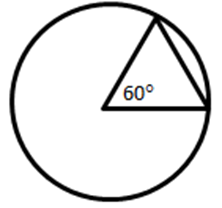
\includegraphics{49}

In the diagram above, the perimeter of the triangle is 9. What is the circumference of the circle?

\begin{enumerate}[label=(\Alph*)]
\item $3\pi$
\item 6
\item $6\pi$
\item 9
\item $9\pi$
\end{enumerate}}
\end{multienumerate}

\newpage
\subsection{SAT Worksheet 9D (Advanced): 6 Questions, 10 Minutes}
\begin{multienumerate}
\mitemxx{The diagonals of a rectangle are equal to twice the length of the shortest side. If $w$ is the shortest side and $l$ is the longer side, which expression represents the value of $l$ in terms of $w$?

\begin{enumerate}[label=(\Alph*)]
\item $\sqrt{2}w$
\item $\sqrt{2}w/2$
\item $\sqrt{3}w$
\item $\sqrt{3}w/3$
\item $\sqrt{5}$
\end{enumerate}}{If the system

\[6x-4y=15\]

\[3x+k^2y=12\]

Represents the equations of perpendicular lines, what must be the value of $k$?

\begin{enumerate}[label=(\Alph*)]
\item $\pm2/3$
\item $\pm 3/2$
\item $\pm\sqrt{2}/2$
\item $\pm2\sqrt{3}/3$
\item $\pm3\sqrt{2}/2$
\end{enumerate}}

\vfill
\mitemxx{The average of 10 numbers is 16. If the average of 6 of the numbers is 8, what is the average of the remaining numbers?

\begin{enumerate}[label=(\Alph*)]
\item 24
\item 26
\item 28
\item 29.5
\item 56
\end{enumerate}}{If $x$ is a positive integer, and

\[\sqrt{x}+\sqrt{2x+1}=x+1\]

What is the value of $2x$?

\begin{enumerate}[label=(\Alph*)]
\item 0
\item 2
\item 4
\item 6
\item 8
\end{enumerate}}

\vfill
\mitemxx{If the greatest common factor of $m$ and $n$ is $q$, then $q$ is also the greatest common factor of $m$ and which expression?

\begin{enumerate}[label=(\Alph*)]
\item $n-1$
\item $2n$
\item $n^2$
\item $n+1$
\item $m-n$
\end{enumerate}}{There is a total of \$2.20 in quarters, nickels, and dimes. If there are twice as many nickels and twice as many dimes as there are quarters, what is the total value of the dimes?

\begin{enumerate}[label=(\Alph*)]
\item \$0.20
\item \$0.40
\item \$0.60
\item \$0.80
\item \$0.90
\end{enumerate}}
\end{multienumerate}
\chapter{Algebra Part I}

\subsection{Worksheet 1E: Warm-Up Problems}

\textbf{Write the strategy that is best used to solve the problem and then solve it.}

\begin{multienumerate}
\mitemxx{\basic

A car rental company has two policies. Policy A requires customers to pay a monthly \$75 fee and an additional \$6 for every hour they use the car. Policy B has no monthly fee but requires customers to pay \$11 for every hour they use the car. How many hours does a customer have to drive in a month to make policy A more advantageous than policy B?

\bigskip
Strategy:

\bigskip
Solve:
}{\medium

John places an order at a local pizzeria for $p$ total pizzas. Where $p$ is at least 4 but no more than 6, which inequality represents all possible values of $p$?

\begin{enumerate}[label=(\Alph*)]
\item $|p-5|\leq2$
\item $|p-5|\leq1$
\item $|p-1|\leq6$
\item $|2-p|\leq4$
\item $|2-p|\leq1$
\end{enumerate}

\bigskip
Strategy:

\bigskip
Solve:}

\vfill
\mitemx{\medium

Ella has a group of friends consisting of both 1st and 3rd graders. One day she decides to invite all 8 of them over for a tea party. At the party she plans to bake cookies for all of her friends. Naturally, the 3rd graders can eat 5 cookies each and the 1st graders only eat 2 cookies each. Using this information, Ella estimates how many cookies her friends will eat and then makes 10 extra just in case people eat more. If she made 32 cookies, how many 1st grade friends are coming?

\begin{enumerate}[label=(\Alph*)]
\item 8
\item 7
\item 6
\item 5
\item 4
\end{enumerate}

\bigskip
Strategy:

\bigskip
Solve:}
\end{multienumerate}

\newpage
\section[Functions]{Algebra Topic \#1: Functions}

Connection to previous material learned:

\begin{itemize}
\item If $y=x^2-1$ and $x=-2$ what is the value of $y$? \longline
\item If $y=1-x$ and $y=-2$, what is the value of $x$? \longline
\item A problem-solving strategy to keep in mind: If you have a problem with lots of variables and don't know how to solve it, you should try to \longline the answer choices to help you solve the problem. For example, we could \longline for each variable, plug in this number into the problem and each of the answer choices, and solve to see which solution of the answer choices \longline the solution in the question.
\end{itemize}

\vfill
Functions have the form $f(x)=$ some definition with an $x$, such as $f(x)=x^2-1$. The notation for a function is a letter and $x$ combination, $f(x)$ and $g(x)$. Both can be treated as $y$, so ``If $y=x^2-1$ and $x=-2$, what is the value of $y$?” becomes ``If $f(x)=x^2-1$ and $x=-2$, what is the value of $f(x)$?'' and ``if $g(x)=1-x$ and $g(x)=-2$, what is the value of $x$?'' \longline

\vfill
The variable in the parentheses is what gets plugged in to the definition. For example, $f(2)=x^2-1$ can be written as $f(2)=$\longline. Now solve $f(2)=x^2-1$ to get an answer of \longline. You may also get questions that give you the value of the output, f(2), and ask you to find the variable, $x$. Therefore, if the value of $f(x)=3$ and the definition of $f(x)=x^2-1$, what is $x$? \longline.

\vfill
Sometimes you may be given the input and output ($x$ and $f(x)$) and then be expected to find the equation or part of an equation, such as a coefficient or a constant in the equation. To do so, plug in the numbers given in the problem and solve for the unknown.

\vfill
What should you do when you have two functions in the same problem? The output of one function can solve as the input for another function. For example, if $f(x)=x+1$ and $g(x)=2x$, then what is $g(f(x))$? To find this, start with the \longline. In this example, we can find the value of $f(x)$. Then plug this output into the x value of the function on the outside. Using $f(x)$ and $g(x)$ defined earlier in this paragraph, what is $f(g(2))$? What is $g(f(2))$? \longline

\vfill
The SATs will also define novel functions with a weird symbol $-$ such as $\diamond$, $\uparrow$, \$, etc. $-$ and ask you to then solve for some part of the function. These are often called ``weird symbol problems''. Most of the time, you need to solve the equation that they give you using the number in the problem. For example, if $\#g\#=g+1$, then what is \#5\#? \longline If $\#g\#h\#=gh-h$, then what is \#5\#6\#? \longline.

\newpage
\subsection{SAT Worksheet 2E: 8 Questions, 10 Minutes}

\begin{multienumerate}
\mitemxx{\basic

If $f(x)=(3-4x^2)/-1$, what is the value of $f(-1)$?

\begin{enumerate}[label=(\Alph*)]
\item $-1$
\item 0
\item 1
\item 2
\item 4
\end{enumerate}
}{\basic

If $f(x)=x^2-1$, what is the value of $2f(5)$?
\begin{enumerate}[label=(\Alph*)]
\item 4
\item 10
\item 24
\item 48
\item 25
\end{enumerate}}

\vfill
\mitemxx{\medium

If $f(p)=(2p)^2-5$ and $f(p)=10$, what is the value of $f(p^2)$?}{\medium

Let $f$ be a function such that $f(x)=c|x^3|+12$ where $c$ is a constant. If $f(-1)=4$, what is the value of $f(5)$?}

\vfill
\mitemxx{\advanced

If $f(x)=-2x+8$, give a value of $x$ for which $f(x)=2f(x)$.}{\advanced

In the function $g(x)=ax^2+5$, $a$ is a constant. When graphed on the $xy$-coordinate plane, one of the points on the line is $(4,6)$. What is the value of the constant $a$?}

\vfill
\mitemxx{\advanced

If $f(x)=x^2-2x+9$ and $g(x)=|x|+$, what is $f(g(-10))$?}{\advanced

If $f(x)=x+4$ and $g(x)=5(x)-2(x)$, what is the positive difference between $f(g(2))$ and $g(f(2))$?}
\end{multienumerate}

\vfill
\newpage
\section{Functions with Charts and Graphs}

Sometimes, there are questions with charts containing the input, x, and the corresponding output, f(x). These questions will usually ask you to find the equation that fits the line of the \longline.

\bigskip
In order to solve these types of problems, you will need to plug x and f(x) into the equation given or in the answer choices. Most of the time, you will need to check that the equation with \longline points rather than just one because more than one answer choice will work for one pair of $x$ and $f(x)$ values.

\bigskip
Example \#1: given the chart of the quadratic function below, what is the general equation of the function?

\bigskip
\begin{spacing}{1.5}
\begin{tabularx}{\textwidth}{|*6{@{}>{\centering\arraybackslash$}X<{$\arraybackslash}|}}\hline
x & -2 & -1 & 0 & 1 & 2\\\hline
f(x) & 5 & 2 & 1 & 2 & 5\\\hline
\end{tabularx}
\end{spacing}

\section{Functions and Graphs}

Functions may be graphed on an $xy$-coordinate plan. Remember that in the form of the function $f(x)$, the value of $x$ in the $f(x)$ is plotted on the $x$-coordinate and the value of $f(x)$ is treated as the $y$-coordinate.

\begin{enumerate}
\item Graph the quadratic function given in example \#1 above:

\plane

\item What is the minimum of the function?
\item Use the graph to find $f(2)$.
\item Use the graph to find $x$ when $f(x)=2$
\end{enumerate}

The SATs will often ask about transformations of the graph of a function. Determine how each of the following transformations will affect a function. Then, draw the transformation of the function $f(x)=x^2+1$ on the grid beside the transformation.

\begin{multicols}{2}
\textbf{Reflection in the $\boldsymbol{x}$-axis}

\bigskip
For example: $f(x)\rightarrow-f(x)$

\vfill
\columnbreak
\plane
\end{multicols}

\hrulefill
\begin{multicols}{2}
\textbf{Vertical Translation}

Move $f(x)$ up or down on the $y$-axis

\bigskip
For example: $f(x)\rightarrow f(x)+2$

\vfill
\columnbreak
\plane
\end{multicols}

\hrulefill
\begin{multicols}{2}
\textbf{Horizontal Translation}

Move $f(x)$ to the left or the right (move the function along the $x$-axis)

\bigskip
For example: $f(x-2)$

\vfill
\columnbreak
\plane
\end{multicols}

\newpage
\begin{multicols}{2}
\textbf{Vertical Stretch/Compression}

\bigskip
For example: $f(x)\rightarrow2f(x)$

\vfill
\columnbreak
\plane
\end{multicols}

\hrulefill
\begin{multicols}{2}
\textbf{Horizontal Stretch/Compression}

\bigskip
For example: $f(x)\rightarrow f(2x)$

\vfill
\columnbreak
\plane
\end{multicols}

\newpage
\subsection{SAT Worksheet 3E: 6 Questions, 8 Minutes}

\begin{multienumerate}
\mitemxx{\basic

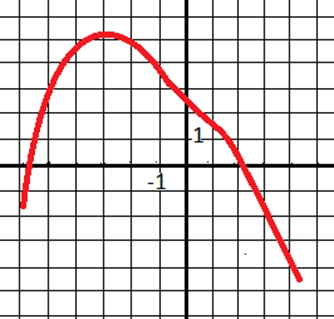
\includegraphics{50}

Based on the graph of the function $g$ above, for what values of $x$ is $g(x)$ positive?}{\basic

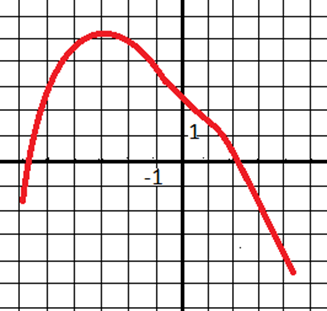
\includegraphics{51}

The graph above contains the function $f(b)$. If $f(b)=0$, which of the following is a possible value for $b$?

\begin{enumerate}[label=(\Alph*)]
\item $-1$
\item 0
\item 1
\item 2
\item 5
\end{enumerate}}

\vfill
\mitemxx{\medium

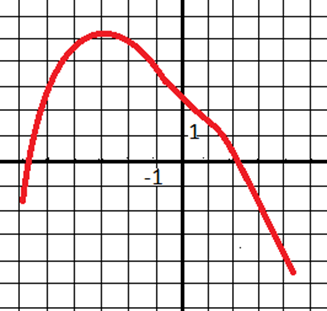
\includegraphics{51}

The graph above contains the functions $f(x)$ and $g(x)$. If $g(5)=b$, what is the value of $f(b)$?
}{\medium

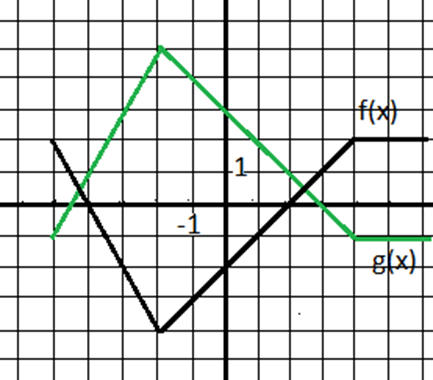
\includegraphics{52}

The graph above contains the functions $f(x)$ and $g(x)$. Which of the following equations best represents the relationship between $f(x)$ and $g(x)$?

\begin{enumerate}[label=(\Alph*)]
\item $f(x)=-g(x)+1$
\item $f(x)=-g(x-1)$
\item $f(x)=-g(x)$
\item $f(x)=2g(x)$
\item $f(x)=-g(x)-1$
\end{enumerate}}

\vfill
\mitemxx{\advanced

If $f(x)=x^2-2x$, then how will a graph of $f(x+2)$ differ from a graph of $f(x)$?

\begin{enumerate}[label=(\Alph*)]
\item Stretched by a factor of 2
\item Shifted right by 2
\item Increased by 2
\item Compressed by a factor of 2
\item No change
\end{enumerate}
}{\advanced

Let the function $g$ be defined by $g(a)=-3a$. If $3/5g(a^{1/2})=12$, what is the value of $a$?}
\end{multienumerate}

\section[Word Problems]{Functions and Equations in Word Problems}

Given the equation and asked to solve for the input or output or you may be given a problem and be asked to choose the function that best represents the problem.

\bigskip
There are 2 general types of questions of this type on the SATs:

\begin{enumerate}
\item A situation may be modeled by a function and will ask you to solve for the value of the function (so you would solve for f(x)) or could ask you what value of x will produce a certain value of y (so you would solve for x)

\vfill
\item They may give a situation and ask you to choose the equation that best models it. The equation may have numbers and variables. The strategy for solving these is to solve or check your answer by plugging in real numbers for each of the variables and solving.
\end{enumerate}

\vfill
Example \#1: To rent a lane for a party at a bowling alley is \$30 per hour plus \$10 per person attending the party. Which of the following functions models the total cost, in $d$ dollars, to rent the room for a 2 hour party for $n$ people?

\begin{enumerate}[label=(\Alph*)]
\item $f(n)=40n$
\item $f(n)=30+10n$
\item $f(n)=60+10n$
\item $f(n)=30n+10$
\item $f(n)=70n$
\end{enumerate}

This question is fairly straightforward. However, what if there was a twist so that there were more variables?

\bigskip
Example \#2: To rent a lane for a party at a bowling alley is \$f per hour plus \$x per person attending the party. Which of the following functions models the total cost, in $d$ dollars, to rent the room for an $m$ hour party for $n$ people?

\begin{enumerate}[label=(\Alph*)]
\item $f(n)=fmn$
\item $f(n)=f + xn$
\item $f(n)=mf + xn$
\item $f(n)=(f+x)n$
\item $f(n)=mfx+n$
\end{enumerate}

Example \#2 looks much more difficult than Example \#1, however it is really the same problem but with variables instead of numbers. We can use a strategy to help us solve or check our answer for example \#2.

\vfill
\textbf{SAT Math Strategy:} When you have a problem and answer choices with variables and you don't know how to solve it, assign one number to each variable and solve the problem in the question and the answer choices. Each of the numbers should be relatively small so that they are easy to work with and different from the numbers you assign other variables. Your answer is the answer the choice that matches the value in the question. 

\bigskip
For example \#2, we can assign $f=5, x=2$, and $m=1$. So we have a 1 hour party for 2 people with a room cost of \$5 per hour. Therefore, the total cost should be \$7. Now we need to calculate the result of each of the answer choices using $f=5, x=2$, and $m=1$ to see which answer choice(s) give us \$7. If there is more than one answer choice that gives you the numerical answer that you are looking for, then you should pick different numbers for each variable and re-solve for the answer choices that originally matched what you are looking for.

\begin{enumerate}[label=(\Alph*)]
\item $f(n)=fmn=5*2*1=10$

We can eliminate this as the possible correct answer.

Now, solve this for each of the other possible answer choices.

\item $f(n)=f+xn$
\item $f(n)=mf+xn$
\item $f(n)=(f+x)n$
\item $f(n)=mfx+n$
\end{enumerate}

\vfill
\newpage
\subsection{SAT Worksheet 4E: 4 Questions, 5 Minutes}

\begin{multienumerate}
\mitemxx{\basic

A department store is having a sale on shoes. The first pair of shoes that you buy is \$30 and each subsequent pair of shoes are then 20\% off the original \$30 price. Which of the following functions describes the cost, in dollars, of the price of buying $n$ total shoes?

\begin{enumerate}[label=(\Alph*)]
\item $f(n)=30(n-2)$
\item $f(n)=30+48(n-2)$
\item $f(n)=30+24(n-2)$
\item $f(n)=30+6(n-2)$
\item $f(n)=30+12(n-2)$
\end{enumerate}}{\basic

The value of a car $x$ years after purchase in dollars, $d$, is represented by the function $d(x)=10,000(0.81)^x$. In how many years after purchase will the car be worth \$6,561?

\begin{enumerate}[label=(\Alph*)]
\item 0
\item 1
\item 2
\item 3
\item 5
\end{enumerate}}

\vfill
\mitemxx{\medium

An object is launched at 19.6 meters per second (m/s) from a 58.8 meter tall platform. The equation for the object's height at time $t$ seconds after launch is $s(t) = -4.9t^2 + 19.6t + 58.8$, where $s$ is in meters. When does the object strike the ground?
}{\advanced

At a party, $p$ sisters decide to contribute to their mother's present that costs a total of s dollars. One sister, Anna, contributes $x$ dollars and the rest of the sisters contribute equally to the present. Which of the following represents the amount in dollars that each of the sisters except Anna contributed?

\begin{enumerate}[label=(\Alph*)]
\item $sx/(p-1)$
\item $s/p$
\item $(p-1)/s$
\item $(s-x)/(p-1)$
\item $(s/(p-1))x$
\end{enumerate}}
\end{multienumerate}
\chapter{Algebra Part II}

\subsection{SAT Worksheet 1F: Warm-Up Problems}

\textbf{Solve the following questions:}

\begin{multienumerate}
\mitemxx{\basic

Winifred makes \$250 a week and deposits 10\% of that into her savings account. Jenny makes \$300 a week and deposits 20\% of it into her savings. At the beginning of the month of February, Winifred's account already has \$1620 and Jenny's has \$1200. At the end of which month will they have the same amount of money in their savings account? (Assume each month to be four weeks)

\begin{enumerate}[label=(\Alph*)]
\item March
\item April
\item May
\item June
\item July
\end{enumerate}}{\medium

Steven has been working hard to try to make a specific weight bracket in wrestling that requires him to weigh somewhere between 160 and 174 pounds. If Steven's staring weight was 182 pounds and $w$ represents the amount of weight Steven loses, which inequality expresses all the possible values of $w$?

\begin{enumerate}[label=(\Alph*)]
\item $|w-22|\leq8$
\item $|w-15|\leq8/22$
\item $|w-22|\leq14$
\item $|w-167|\leq7$
\item $|w-15|\leq7$
\end{enumerate}}

\vfill
\mitemxx{\medium

Choco's Chocolate sells chocolate bars for \$3 and fudge for \$5. Max spent a total of \$27 on his recent trip to Choco's Chocolate and returned home with a bag of 7 items containing both chocolate bars and fudge. How much money did Max spend on fudge?

\begin{enumerate}[label=(\Alph*)]
\item \$9
\item \$10
\item \$12
\item \$15
\item \$20
\end{enumerate}}{\advanced

Tim's score on a test was five times the square root of Jane's and Mary's score was twice as much as Tim's. If Mary got a 90 on the test, what is the difference between Jane's and Tim's score?

\begin{enumerate}[label=(\Alph*)]
\item 36
\item 45
\item 9
\item 81
\item 26
\end{enumerate}}
\end{multienumerate}

\newpage
\section{Patters and Sequences}

A remainder is the amount left over after \longline. For example, six will divide into 19 three times with a remainder of \longline.
We can usually use one of two strategies to solve these types of problems.

\vfill
\textbf{Strategy \#1:} If a remainder problem contains a variable problem, then we can

\longline that fits the parameters and then use this number to solve for what the problem is asking. 

\bigskip
For example: When 2m is a divided by 4, the remainder is 5. What will the remainder be when $3m$ is divided by 10?

\vfill
\textbf{Strategy \#2:} Then you need to come up with \longline and solve for the \longline in order to solve. 
For example, When 48 is divided by a positive integer $n$, the remainder is 4. How many values of $n$ are possible?

\vfill
We are also going to use a strategy similar to Strategy \#2 in order to solve problems that repeat numbers, symbols, etc. by using divisibility rules. We are particularly interested in the  \longline.

\bigskip
For example, A fashionista is laying out her colored scarves. She first lays down 2 red scarves, then 3 blue scarves, then 1 green scarf, then 2 orange scarves, then 1 pink scarf. She repeats this pattern until she has laid out all 1,000 scarves. What color is the 782\textsuperscript{nd} scarf?

\begin{enumerate}[label=(\Alph*)]
\item red
\item blue
\item green
\item orange
\item pink
\end{enumerate}

\begin{enumerate}
\item Start by writing \longline iterations of the pattern on top of each other:
\vfill\item \longline the end of each line
\vfill\item You will see that you are counting up by \longline occurring in the first line
\vfill\item Divide the \longline by the \longline.

Find the \longline.
\vfill\item Start at the beginning of the pattern. Count each unique item in the pattern until you reach the same number as the \longline. This item in the pattern is the \longline.
\end{enumerate}

Example \#2: There are 5 ducks in a row behind the mother ducks, Ariel, Boston, Carl, Devin, and Edward. Every day, the ducks take a turn swimming behind the mother so it is Ariel's turn, then Boston's turn, then Carl's turn, then Devin's turn, then Edward's turn. If Boston swims behind his mother on the first day, who will be swimming behind the mother on the 42\textsuperscript{nd} day?

\begin{enumerate}[label=(\Alph*)]
\item Ariel
\item Boston
\item Carl
\item Devin
\item Edward
\end{enumerate}

\vfill
Example \#3: Every day, Steven runs one errand or completes one chore. On the first day, he goes to the grocery store. On the next day, he goes to the laundry mat, and on the next day, he goes to the pharmacy. On the next day, Steven goes to the car mechanic, and on the next day, he cleans the house. After this, he repeats his chore list (so the day after cleaning the house, he goes to the grocery store). One day that he went to the car mechanic, he went to the movies immediately afterwards. Which of the following could be the number of days he did chores prior to the day that he decided to go to the movies? \textbf{[Note: In previous problems, it has given you the total number and wants you to find the unique item. This problem gives you the unique item, that he goes to the movies, and wants you to use divisibility rules to find the total number. You can use steps \#1-5 above, but you need to reverse them.]}

\begin{enumerate}[label=(\Alph*)]
\item 30
\item 74
\item 143	%so much was wrong with this question but it should be fixed now
\item 271
\item 362
\end{enumerate}

\vfill
Example \#4: $6, 11, 16, 21, \ldots$

\bigskip
Each term in the sequence after the first term is 5 more than the term before it. The 45\textsuperscript{th} term than the 37\textsuperscript{th} term? \textbf{The challenge is to solve this without solving for the 37\textsuperscript{th} and the 45\textsuperscript{th} term.}

\begin{enumerate}[label=(\Alph*)]
\item 18
\item 25
\item 37
\item 38
\item 40
\end{enumerate}

\vfill
We will use the idea of writing out the possible items to solve problems that ask about the minimum number of items selected in order to guarantee some situation. 

\bigskip
For example, there are 144 marbles in a box. There are 24 marbles of each of the following colors: red, blue, green, white, black, and gray. Tom randomly selects marbles from the box.

\begin{enumerate}[label=\alph*)]
\item What is the minimum number of marbles Tom needs to select in order to guarantee that he gets at least two marbles of the same color? 

\bigskip
To solve this, we need to think of the \longline. In this scenario, he selects \longline before he selects a second marble of any color. 


\vfill
\item What is the minimum number of marbles Tom needs to select in order to guarantee that he gets at least two marbles of the same color?
\end{enumerate}

\vfill
\newpage
\subsection{SAT Worksheet 2F: 4 Questions, 5 Minutes}

\begin{multienumerate}
\mitemxx{\basic

When $k$ is divided by 10, the remainder is 5. $k$ could have which of the following as factors?

\begin{enumerate}[label=\Roman*.]
\item 2
\item 3
\item 5
\end{enumerate}

\begin{enumerate}[label=(\Alph*)]
\item I only
\item II only
\item I and II only
\item II and III only
\item I, II, and III
\end{enumerate}}{\basic

$7.03615036150361\ldots$

The decimal number above continues to repeat to the 100\textsuperscript{th} digit to the right of the decimal point. What is the 20\textsuperscript{th} digit to the right of the decimal place?

\begin{enumerate}[label=(\Alph*)]
\item 0
\item 3
\item 6
\item 1
\item 5
\end{enumerate}}

\vfill
\mitemxx{\medium

$7.036150361503615\ldots$

The decimal number above continues to repeat until the 100\textsuperscript{th} digit to the right of the decimal point. What is the product of values from the 90\textsuperscript{th} digit to the 92\textsuperscript{nd} digit to the right of the decimal place?}{\advanced

$1.566566665\ldots$

In the number above, the decimal number contains only 5's and 6's. The first 5 is followed by two 6's, the second 5 is followed by four 6's, and the $n$\textsuperscript{th} 5 is followed by $2n$ number of 6's. How many 6's are between the 47\textsuperscript{th} number 5 and the 51\textsuperscript{st} number 5?}
\end{multienumerate}

\vfill
\newpage
\section{Probability}

In general, probability of an event is occurring is defined as:

\vfill
The most difficult type of probability questions are when multiple events are occurring because you must take into account the wording of the question to give you a clue as to whether the events are happening together or separately and also if the items are getting replaced or not (as this will affect the denominator when you are solving the problem). 
Probability is a number between \shortline and \shortline. \shortline represents the sum of all of the events that could happen. For example, on a fair two-sided coin, the options from one coin flip are getting a tails or a head (and nothing else). The probability of getting the tail side is ½ and the probability of getting the head side is $1/2$ and$1/2 + 1/2 =1$.

\vfill
If you want to know the probability of an event not happening, you will need to find the probability of it happening and subtract this probability from \shortline. This is called the \longline.

\vfill
\longline events are when the results of the first event affects the probability of the second event occurring or not occurring.

\vfill
\longline events are when the results of the first event affects the probability of the second event occurring or not occurring.

\vfill
If you want to know the probability of two independent events happening, then

\longline the probabilities. For example, you would use this method when you select a ball from a jar, put it back in the jar, and then choose another ball (called choosing with replacement).

\vfill
If you want to know the probability of two dependent events happening, then you will need to \longline the probability of the second event based on the first event happening. For example, you would use this method when you select a ball from a jar, and then choose another ball without putting the first ball back (called choosing without replacement).  If the probability of choosing a green ball is 7/10 and you want to know the probability of choosing two green balls in a row without replacement, then you calculate the probability of the first ball being green, 7/10, and the second ball being green with the first green ball removed, which is $(7 - 1)/(10 - 1) = 6/9$. Therefore, the probability of getting two green balls in a row without replacement of the first ball would be $7/10 \cdot 6/9 = 42/90$.

\vfill
If you want to know the probability of neither happening, you will need to find the probability of either happening and subtract this probability from \shortline. This is called the \longline.

\vfill
\newpage
We will now use one example and see how many ways a problem can be asked. In each case, there are 10 red balls and 12 blue balls in Jar $A$ and 3 red balls and 9 blue balls in Jar $B$. Show your work when solving for each problem so that you can see the differences between the words and problem-solving steps for it. 

\begin{enumerate}[label=\alph*)]
\item A person picks one ball from Jar A, records the color, puts it back in the jar and then picks a ball from Jar B. What is the probability that the first ball is red or the second ball is blue?
\vfill\item A person picks one ball from Jar A, records the color, and picks a ball from Jar B. What is the probability that the first ball is red and the second ball is blue?
\vfill\item What is the difference in wording between a) and b)? How does this account for different approaches that you need to use to solve the two problems?
\vfill\item A person picks one ball from Jar A, records the color, and picks another ball from Jar A without putting the first ball back in the jar. What is the probability that both balls selected are red?
\vfill\item A person picks one ball from Jar A, records the color, and picks another ball from Jar A without putting the first ball back in the jar What is the probability that both balls selected are the same color?
\vfill\item What is the difference in wording between d) and e)? How does this account for different approaches that you need to use to solve the two problems?
\vfill\item g)	A person picks one ball from Jar A, records the color, replaces the first ball and picks another ball from Jar A. What is the probability that both balls selected are red?
\vfill\item What is the difference in wording between d) and g)? How does this account for different approaches that you need to use to solve the two problems?
\end{enumerate}

\vfill
\newpage
\subsection{SAT Worksheet 3F (Basic): 6 Questions, 8 Minutes}

\begin{multienumerate}
\mitemxx{1.	Ms. Ziggy has a jar with 6 red marbles, 4 blue marbles, and 5 green marbles. If a student removes two marbles, one at a time, what is the probability that a student will randomly pick 2 red marbles in a row?

\begin{enumerate}[label=(\Alph*)]
\item 1/7
\item 2/7
\item 2/5
\item 3/5
\item 2/3
\end{enumerate}}{Sally has 3 pairs of color shoe laces, 2 pairs of shoes, and 4 pairs of color socks. How many combinations of laces, shoes, and socks does Sally have?

\begin{enumerate}[label=(\Alph*)]
\item 9
\item 10
\item 11
\item 12
\item 24
\end{enumerate}}

\vfill
\mitemxx{

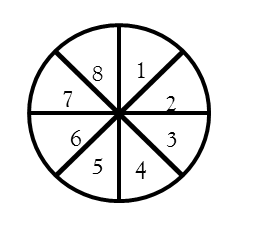
\includegraphics{54}

What is the probability of landing on a prime number on the spinner above?

\begin{enumerate}[label=(\Alph*)]
\item 1/4
\item 3/8
\item 1/2
\item 5/8
\item 3/4
\end{enumerate}
}{What is the missing term in the following sequence?

$64, -32, 16, \shortline, 4, -2, 1$

\begin{enumerate}[label=(\Alph*)]
\item 9
\item 8
\item -8
\item 12
\item -12
\end{enumerate}}

\vfill
\mitemxx{Accounts at General Bank Savings ATMs require four digits pins such that no digit is repeated. How many possible combinations of pins are possible?

\begin{enumerate}[label=(\Alph*)]
\item 1920
\item 3024
\item 5040
\item 6561
\item 10,000
\end{enumerate}}{If there are 4 queens and 4 kings in a standard deck of 52 cards, what are the odds of choosing a queen or a king?

\begin{enumerate}[label=(\Alph*)]
\item 1/13
\item 2/13
\item 4/13
\item 1/169
\item 2/169
\end{enumerate}}
\end{multienumerate}

\newpage
\subsection{SAT Worksheet 4F (Medium): 6 Questions, 9 Minutes}

\begin{multienumerate}
\mitemxx{The sum of the angles of an n-sided regular polygon can be found by adding 180 to the sum of the angles of a regular polygon of one less side. If the sum of the angles of a square is 360, what is the value of one angle of a 10-sided regular polygon?

\begin{enumerate}[label=(\Alph*)]
\item 72
\item 80
\item 120
\item 144
\item 162
\end{enumerate}}{A hat contains the numbers from 1 to 20. What is the probability of picking out a number that is not a perfect square?

\begin{enumerate}[label=(\Alph*)]
\item 0.15
\item 0.20
\item 0.75
\item 0.80
\item 0.85
\end{enumerate}}

\vfill
\mitemxx{

\medskip
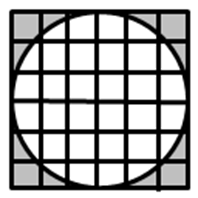
\includegraphics{55}

A circle of radius 3 units is inscribed in a square. If a dart that occupies 1 square unit is tossed at the board, state the odds of the dart landing within the circle to the nearest hundredth.}{What is the smallest possible three digit integer whose prime factors are non-repeating?

\begin{enumerate}[label=(\Alph*)]
\item 120
\item 144
\item 210
\item 330
\item 378
\end{enumerate}}

\vfill
\mitemxx{If $n$ is a positive integer, which of the following expressions does not necessarily have a factor of 3?

\begin{enumerate}[label=(\Alph*)]
\item $3n+3$
\item $6n$
\item $6(n-1)$
\item $3^n$
\item $n^3$
\end{enumerate}}{The largest number of a set of four consecutive integers is the smallest number of a different set of four consecutive integers. What is the difference between the smallest number of the first set to the largest number of the second set?

\begin{enumerate}[label=(\Alph*)]
\item 4
\item 5
\item 6
\item 7
\item 8
\end{enumerate}}
\end{multienumerate}

\newpage
\subsection{SAT Worksheet 5F (Advanced): 6 Questions, 10 Minutes}

\begin{multienumerate}
\mitemxx{If the first term of a sequence is $n$, and each subsequent term is found by adding 1 more than the previous term, which expression represents the sixth term?

\begin{enumerate}[label=(\Alph*)]
\item $n+5$
\item $6n$
\item $6n+5$
\item $6n+15$
\item $6n+21$
\end{enumerate}}{If $n$ is a positive integer, which of the following expressions cannot represent a prime number?
\begin{enumerate}[label=(\Alph*)]
\item $n^2-1$
\item $n+1$
\item $2n+1$
\item $2(n-1)+6$
\item $2^n-1$
\end{enumerate}}

\vfill
\mitemxx{For which of the following numbers is the sum of its factors, not including the number itself?

\begin{enumerate}[label=(\Alph*)]
\item 4
\item 10
\item 12
\item 24
\item 28
\end{enumerate}}{Which of the following expressions does not represent the sum of four consecutive integers?

\begin{enumerate}[label=(\Alph*)]
\item $4n-1$
\item $4n$
\item $4n+2$
\item $4n+3$
\item $4n+4$
\end{enumerate}}

\vfill
\mitemxx{A number, $n$, is divided by 3 and has a remainder of 1. When the quotient is divided by 3, the remainder is 2. For any positive integer $k$, which of the following expressions represents all possible values of $n$?

\begin{enumerate}[label=(\Alph*)]
\item $3k-1$
\item $3k+2$
\item $9k+7$
\item $9k$
\item $9k-1$
\end{enumerate}}{Let $n$ be a number with $d$ factors. If $d$ is an odd number, which of the following must be true?


\begin{enumerate}[label=\Roman*.]
\item $n/d$ must also be odd
\item $n$ is a perfect square
\item $n-d$ must be odd
\end{enumerate}

\begin{enumerate}[label=(\Alph*)]
\item I only
\item II only
\item III only
\item I and II
\item I, II, and III
\end{enumerate}}
\end{multienumerate}
\chapter[Statistics, and Probability]{Problem-Solving Strategies for Data Analysis, Statistics, and Probability}

\subsection{SAT Worksheet 1G: Warm-Up Problems}

\textbf{Strategies and content practice:} Write which strategy or strategies that you want to use to solve the following word problems. Then, solve the problem.

\begin{multienumerate}
\mitemxx{\medium

Maria makes a bet with her friends that if she pulls two cards out of a deck without replacing them, the first will be a red number card (2-10) and the second will be a black face card (Jack, Queen, King, Ace). What are the odds of Maria winning this bet?

\begin{enumerate}[label=(\Alph*)]
\item 12/221
\item 9/169
\item 11/26
\item 25/102
\item 13/200
\end{enumerate}}{\medium

If a fair six-sided dice is rolled twice and predictions are made on the outcome. Which of the following predictions has the highest chance of being true?

\begin{enumerate}[label=(\Alph*)]
\item Five will be rolled twice
\item An even number will be rolled first and an odd number will be rolled second
\item Two even numbers will be rolled
\item The sum of the two numbers will be either 8 or 9
\item The sum of the two numbers will be less than 7
\end{enumerate}}

\vfill
\mitemxx{\advanced

Marcus has recently been told by his doctor that he should try to eat one fruit, one vegetable, and one meat every day. For fruit, Marcus loves strawberries, bananas, and blueberries. For vegetables he only likes corn and carrots. For meat, Marcus enjoys chicken, beef, pork, and lamb. If Marcus tries a different combination every day of fruit, vegetables, and meat, how many possible combinations will be available to pick from on the beginning of the fifth day?}{\advanced

What is the greatest number of pieces that can be made from a cylinder using only three cuts (without moving any of the pieces)?

\begin{enumerate}[label=(\Alph*)]
\item 5
\item 6
\item 7
\item 8
\item 9
\end{enumerate}}
\end{multienumerate}

\newpage
\section[Visual Data]{Visual Data, Data Analysis, and Statistics}

Examples:

\centerline{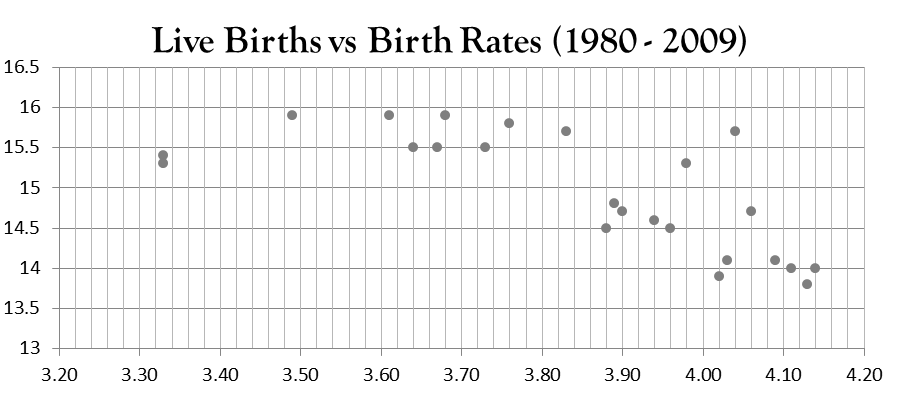
\includegraphics{56}}

\begin{multienumerate}
\mitemxx{\basic

The graph above represents the number of live births (in millions) versus the birth rates (number of births per 1000 in a population) in the US from 1980 to 2009. Which of the following is not likely to be a point on the graph?

\begin{enumerate}[label=(\Alph*)]
\item $(3.3,20)$
\item $(3.8,15)$
\item $(3.9,14.3)$
\item $(4.1,16)$
\item $(4.2,16.5)$
\end{enumerate}}{\medium

Which of the following statements can be inferred by the information on the graph above?

\begin{enumerate}[label=(\Alph*)]
\item Birth rates are decreasing every year
\item The number of live births are increasing every year
\item The birth rate is decreasing as the number of live births is increasing
\item The total population in the US is decreasing every year
\item More families are adopting every year
\end{enumerate}}
\end{multienumerate}

\hrulefill

The SATS will include summaries of data in the form of tables, charts, and graphs.

\begin{itemize}
\item Basic questions will ask to you to find information from the visual given. Oftentimes, you will need to perform a basic operation on the numbers that you are pulling from the data, such as adding products from one year to another year or converting the percentages on a circle graph (pie chart) to actual numbers.
\vfill\item More difficult questions can be difficult for the following reasons: 1) The question asks you to perform a more complicated operation based on information given the visual or 2) The question or the visual data includes a component that is extremely tricky. See some of the tricks used (and how to avoid them) in the strategy section below.

\textbf{Strategies for surviving the visual data and data analysis section}

\item Strategy \#1: Read the written information. This may include the main title, the $x$-axis title, and the $y$-axis title. \textit{Pay particular attention to the scaling information found immediately after the titles. It is possible (and probable on the more difficult problems) that the $x$- and $y$-axes will have different scaling.}

\vfill
\item Strategy \#2: When a question is asked about percent increase or decrease, remember that the change is relative. This means that in a bar graph, a relatively small bar becoming only slightly smaller might still be a larger percentage increase than a huge bar turning into a smaller bar. Why does this phenomenon occur? (Hint: think about the general equation for percentage increase or decrease.) \hrulefill

\vfill
\item Strategy \#3: Identify what you are solving for in the question before you solve the problem, and after you have solved for an answer, check to make sure that your answer actually represents what you were asked to solve for in the question.
\end{itemize}

\vfill
\newpage
\subsection{SAT Worksheet 2G: 6 Questions, 8 Minutes}

\begin{enumerate}
\centerline{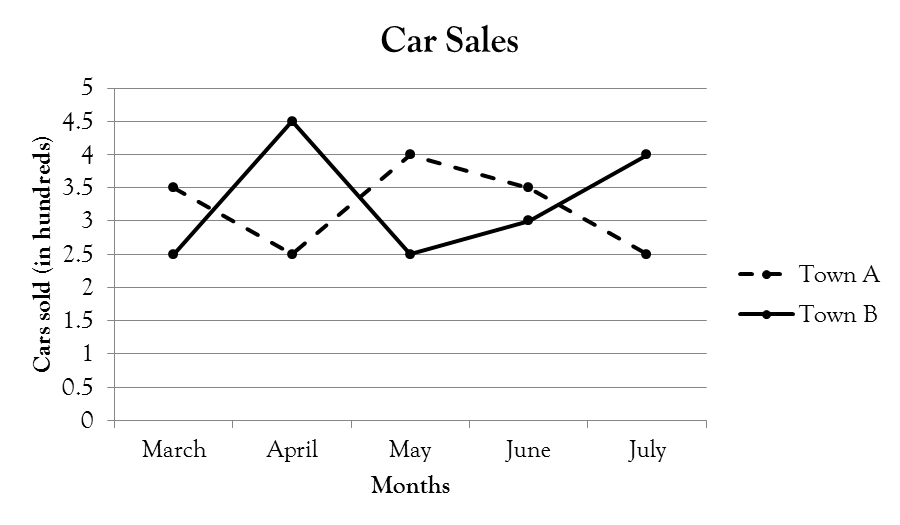
\includegraphics{57}}

\item \basic

The chart above shows the car sales of Town A and Town B over a four month span. During which month is the difference between the car sales in each town the greatest?

\begin{enumerate}[label=(\Alph*)]
\item March
\item April
\item May
\item June
\item July
\end{enumerate}

\vfill
\item \basic

How many more cars were sold in Town B than Town A during the month of July?

\begin{enumerate}[label=(\Alph*)]
\item 15
\item 100
\item 150
\item 1,000
\item 1,500
\end{enumerate}

\newpage
\centerline{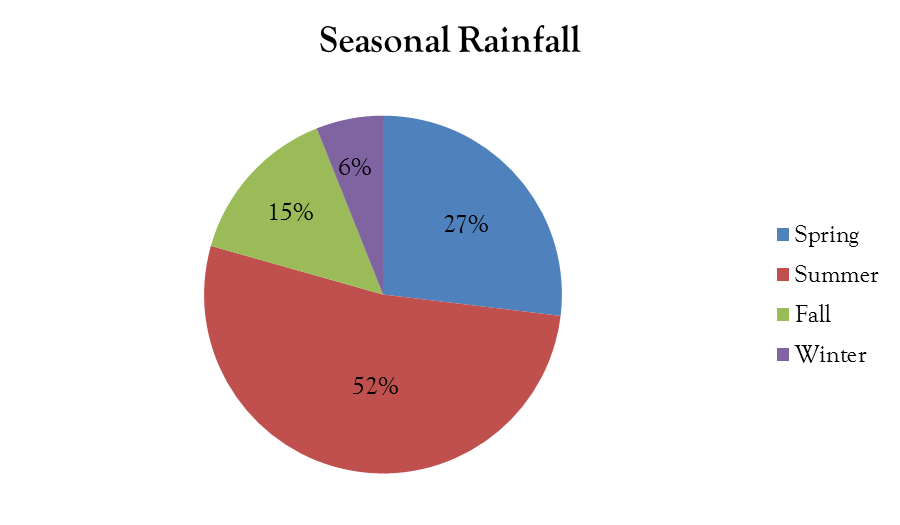
\includegraphics{58}}

\item \medium

Above is a chart of the average (arithmetic mean) seasonal rainfall in Colorado Springs. If the total annual rainfall is 16.54 inches, what is the average amount, in centimeters, of rainfall in the winter?

\begin{enumerate}[label=(\Alph*)]
\item 1 cm
\item 2 cm
\item 4 cm
\item 5 cm
\item 6 cm
\end{enumerate}

\vfill
\newpage
\centerline{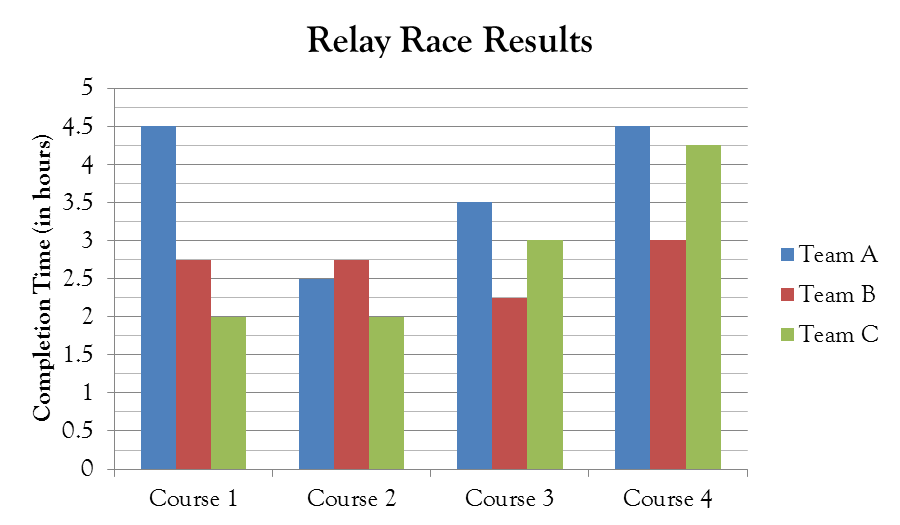
\includegraphics{59}}

\item \medium

Three teams competed in a relay race. How many more minutes did Team B take than Team C on Course 2?

\begin{enumerate}[label=(\Alph*)]
\item 25\%
\item 33\%
\item 75\%
\item 125\%
\item 133\%
\end{enumerate}

\vfill
\item \advanced

In what percent did the average time of Team C complete in the average time of Team A?

\begin{enumerate}[label=(\Alph*)]
\item 25\%
\item 33\%
\item 75\%
\item 125\%
\item 133\%
\end{enumerate}

\vfill
\newpage
\centerline{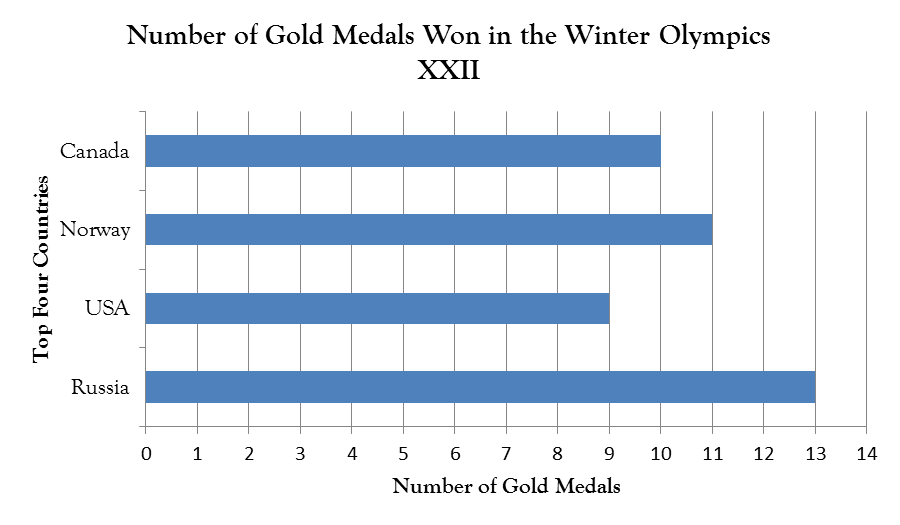
\includegraphics{60}}

\item \advanced

Above is a chart with the countries that received the most number of gold medals in the Winter Olympics XXII. Approximately what percentage of gold medals was won by the two lowest performing countries relative to the top two? (Round to the nearest whole number)

\begin{enumerate}[label=(\Alph*)]
\item 38\%
\item 44\%
\item 69\%
\item 77\%
\item 79\%
\end{enumerate}
\end{enumerate}

\newpage
\section{Averages}

We reviewed the basic formula for averages in the chapter about strategies for algebra, but given that it is a difficult topic, we will discuss it in more depth here. The general formula for averages is:

\vfill
Examples:

\begin{multienumerate}
\mitemxx{\basic

Set A contains $x$ positive integers. If the average (arithmetic mean) is 10, which expression represents their sum?

\begin{enumerate}[label=(\Alph*)]
\item $10-x$
\item $10+x$
\item $10x$
\item $x/10$
\item $10/x$
\end{enumerate}}{\medium

The average (arithmetic mean) of five consecutive even integers is 20. What is the value of the median?

\begin{enumerate}[label=(\Alph*)]
\item 8
\item 10
\item 14
\item 16
\item 20
\end{enumerate}}
\end{multienumerate}

\hrulefill

The more complicated SAT problems on averages usually have to do with solving for\ldots

\textbf{A part of the sum (the numerator of the equation)}- you can do this by using a variable like $x$ to represent the unknown part of the sum and then get $x$ by itself.

\vfill
\textbf{Finding weighted averages}- The average of 50 and 60 is 55 (the middle). However, when you take the average of 50, 60, and 60, the average is closer to \shortline than 60. As a result, you can take into account the number of occurrences weighted by the value of each unique occurrence. This answer will be your sum that can be plugged into the averages formula. 

\vfill
\textbf{The average from visual data}- Here you will find the number of occurrences weighted by the value of each unique occurrence from the chart. Then, solve using the strategy presented in the``finding weighted averages'' category above. 

\vfill
\newpage
\subsection{SAT Worksheet 3G: 6 Questions, 8 Minutes}

\begin{multienumerate}
\mitemxx{\basic The average of $k, k+4$, and $k+8$ is 15. What is the value of $k$?

\begin{enumerate}[label=(\Alph*)]
\item 10
\item 11
\item 15
\item 19
\item 33
\end{enumerate}}{\basic

If the average (arithmetic mean) of 5 numbers is 20, then what is the value of their sum?

\begin{enumerate}[label=(\Alph*)]
\item 15
\item 20
\item 25
\item 50
\item 100
\end{enumerate}}

\vfill
\mitemxx{\medium

Debbie has taken four tests, receiving 78\%, 83\%, 92\%, and 81\%. What grade must she receive on her fifth test in order to have an average of 85\% or better overall?

\begin{enumerate}[label=(\Alph*)]
\item 84\%
\item 85\%
\item 87\%
\item 91\%
\item 92\%
\end{enumerate}
}{\medium

If a set contains five non-negative integers and the average is even, what is the most amount of odd numbers that the set can contain?

\begin{enumerate}[label=(\Alph*)]
\item 0
\item 1
\item 2
\item 3
\item 4
\end{enumerate}}

\vfill
\mitemxx{\advanced

For two positive integers $a$ and $b$, the average of their squares is equal to the square of their average. Which of the following must be true?

\begin{enumerate}[label=\Roman*.]
\item $ab$ is also a perfect square
\item $a=b$
\item $a/b=1$
\end{enumerate}

\begin{enumerate}[label=(\Alph*)]
\item I only
\item II only
\item III only
\item I and III only
\item I, II, and III
\end{enumerate}}{\advanced

\begin{enumerate}[label=\Roman*.]
\item The median of set A is greater than the median of set B
\item The sum of the numbers in set A is smaller than the sum of the numbers in set B
\item Set A shares at least one number in common with set B
\end{enumerate}

\begin{enumerate}[label=(\Alph*)]
\item I only
\item II only
\item III only
\item I and III only
\item I, II, and III
\end{enumerate}}
\end{multienumerate}

\newpage
\subsection{SAT Worksheet 4G (Basic): 5 Questions, 7 Minutes}

\begin{multienumerate}
\centerline{\includegraphics{61}}

\mitemx{The chart above shows the number of students attending the spring dance by class year and gender. How many more girls attended the dance than boys?

\begin{enumerate}[label=(\Alph*)]
\item 5
\item 15
\item 25
\item 30
\item 50
\end{enumerate}}

\vfill
\mitemxx{The sum of 6 numbers is $42m+18n$. What is their average (arithmetic mean)?

\begin{enumerate}[label=(\Alph*)]
\item $7m+3n$
\item $7n+3m$
\item $7m-3n$
\item $36m+12n$
\item $48m-24n$
\end{enumerate}}{Which of the following sets has an average of $2n+1$?

\begin{enumerate}[label=(\Alph*)]
\item ${n-2, n-1, n}$
\item ${n-1, n, n+1}$
\item ${n, n+1, n+2}$
\item ${2n, 2n+1, 2n+2}$
\item ${3n, 3n+2, 3n+4}$
\end{enumerate}}
\end{multienumerate}

\vfill
\newpage
\centerline{\includegraphics{62}}

\begin{multienumerate}
\mitemx{The graph above indicates the number of boxes shipped by Shipping Inc. over four weeks. How many boxes were shipped during week 2?

\begin{enumerate}[label=(\Alph*)]
\item 5.5
\item 30
\item 55
\item 110
\item 120
\end{enumerate}}

\vfill
\mitemx{The average of three positive integers is even. Which of the following must be true?

\begin{enumerate}[label=\Roman*.]
\item The three integers must be even
\item The sum of the three integers must be even
\item Each of the integers must be divisible by three
\end{enumerate}

\begin{enumerate}[label=(\Alph*)]
\item I only
\item II only
\item III only
\item I and II only
\item I, II, and III
\end{enumerate}}
\end{multienumerate}

\vfill
\newpage
\subsection{SAT Worksheet 5G (Medium): 7 Questions, 10 Minutes}

\begin{multienumerate}
\mitemxx{Roberta flips a penny 20 times, landing on heads a total number of 8 times. She flips the same penny another 30 times, landing on heads 21 times. What is the overall average percentage of times the penny landed tails?

\begin{enumerate}[label=(\Alph*)]
\item 40\%
\item 45\%
\item 50\%
\item 55\%
\item 60\%
\end{enumerate}}{

\medskip
\begin{tabular}{|l|c|c|c|}\hline
\multicolumn{4}{|c|}{Approximate Conversions}\\\hline
Number of Inches & 1.2 & 2.4 & 4.8\\\hline
Number of Centimeters & $x$ & 6.1 & 12.2\\\hline
\end{tabular}

\medskip
The table above shows the approximate conversions from inches to centimeters. What is the approximate value of $x$?

\begin{enumerate}[label=(\Alph*)]
\item 1.53
\item 2.54
\item 3.05
\item 3.50
\item 2.87
\end{enumerate}}

\vfill
\mitemxx{Ms. Miller found the average height of her students to be exactly 56 inches tall. If the class consisted of 10 students and the shortest student was a height of 42 inches, what is the lowest possible value for the height of the tallest student?

\begin{enumerate}[label=(\Alph*)]
\item 56.5 in
\item 57.6 in
\item 59.5 in
\item 70.5 in
\item 72.1 in
\end{enumerate}}{If the largest number in a set is equal to the average (arithmetic mean) of the set, which of the following must be true?

\begin{enumerate}[label=\Roman*.]
\item The median is equal to the average
\item The smallest number is equal to the largest number
\item The set contains only one number
\end{enumerate}

\begin{enumerate}[label=(\Alph*)]
\item I only
\item II only
\item III only
\item I and II only
\item I, II, and III
\end{enumerate}}

\vfill
\newpage
\centerline{\includegraphics{63}}

\mitemx{What ratio of the total revenue was brought by the first and second quarter?

\begin{enumerate}[label=(\Alph*)]
\item $2:5$
\item $3:5$
\item $2:3$
\item $1:2$
\item $4:5$
\end{enumerate}}

\vfill
\mitemx{The following graph represents the revenue of Cheerful Toys last year. If the first and second quarter combined yielded a profit of \$200,000, how much revenue was brought in the third and fourth quarter combined?

\begin{enumerate}[label=(\Alph*)]
\item 100,000
\item 200,000
\item 300,000
\item 400,000
\item 500,000
\end{enumerate}}

\vfill
\newpage
\centerline{\includegraphics{64}}

\mitemx{The chart above indicates the total snowfall in Boston during the winter of 2002-2003. Which interval below indicates the greatest rate of increase in snowfall?

\begin{enumerate}[label=(\Alph*)]
\item October to December
\item November to December
\item January to February
\item November to February
\item October to February
\end{enumerate}}
\end{multienumerate}

\vfill
\newpage
\subsection{SAT Worksheet 6G (Advanced): 6 Questions, 10 Minutes}

\begin{multienumerate}
\mitemxx{The average (arithmetic mean) of 1, 3, $x$, 5, and 9 is 4. The average (arithmetic mean) of 2, 4, $y$, 8, and 10 is 6. What is the value of $xy$?

\begin{enumerate}[label=(\Alph*)]
\item 5
\item 8
\item 10
\item 11
\item 12
\end{enumerate}}{The average (arithmetic mean) of 6 numbers is 6. When a seventh number is added, the average is 8. What number was added?

\begin{enumerate}[label=(\Alph*)]
\item 20
\item 30
\item 40
\item 50
\item 60
\end{enumerate}}

\centerline{\includegraphics{65}}

\mitemx{The graph above compares the number of hours students spent studying versus the grades received on their final exam. How many students studied 5 hours or more and received a score of less than 70\%?

\begin{enumerate}[label=(\Alph*)]
\item 1 student
\item 2 students
\item 3 students
\item 4 students
\item More than 4 students
\end{enumerate}}

\newpage
\centerline{\includegraphics{66}}

\mitemx{What is the greatest difference between the average (arithmetic mean) and the least number of boxes shipped in a week?

\begin{enumerate}[label=(\Alph*)]
\item 20
\item 40
\item 50
\item 60
\item 80
\end{enumerate}}

\vfill
\mitemxx{Which of the following is the sum of three consecutive odd integers?

\begin{enumerate}[label=(\Alph*)]
\item 32
\item 33
\item 34
\item 35
\item 36
\end{enumerate}}{The average (arithmetic mean) of five consecutive integers is 3 times more than the median, $c$. Which of the following statements must be true?

\begin{enumerate}[label=\Roman*.]
\item The median is 0
\item The average is 0
\item The sum of the five consecutive integers is 0
\end{enumerate}

\begin{enumerate}[label=(\Alph*)]
\item I only
\item II only
\item III only
\item I and III only
\item I, II, and III
\end{enumerate}}
\end{multienumerate}


\part{SAT Verbal}
\chapter[Multiple Choice Part I]{SAT Writing Multiple Choice Part I}

\section{SAT Worksheet 1A: Warm-Up}
\textit{Today, we will begin studying and unlocking the secrets of doing well on the SAT writing multiple choice sections. To help you and your instructor better assess your background in this area, please answer the following questions.}

\bigskip
Reflect on your most recent written assignments (ranging from one paragraph to multiple pages). What grammatical concepts do you think that you know and execute well?




\vfill

What grammar concepts do you have the most trouble with, that is to say, what types of errors do you make the most frequently? 

\vfill
\pagebreak
\section[Types of Questions]{Types of Questions on the Writing Multiple Choice Section}

The multiple choice section on the writing Section Multiple Choice has three types of questions: error identification, improving sentences, and improving paragraphs.

\bigskip
\textbf{In sentence error questions,} you will read a sentence and circle the part of the sentence that contains the error. There will also be an option for no error. 

\bigskip
For example:

\begin{inparaenum}[A]
\begin{spacing}{1.25}
\begin{tabularx}{\textwidth}{*8{@{}>{\ }c}}
Every day & Maria and & me & go & to the store & \ & to buy milk, & bread, and cheese.  \\\cline{1-1}\cline{3-3}\cline{5-5}\cline{7-7}
\item &  &\item & & \item & &\item &  \\
\end{tabularx}

\begin{tabularx}{\textwidth}{*1{@{}>{\ }c}}
No error
\\\cline{1-1}
\item\\
\end{tabularx}

\end{spacing}

\end{inparaenum}

What would you select here as the error?

\bigskip

\bigskip

\bigskip

\bigskip

\bigskip

\textbf{In sentence improvement questions,} you will be asked to select the best version of a sentence.

\bigskip
For example:\\
Every day, Maria and me go to the store to buy milk, cheese, and bread.
\begin{enumerate}[label=(\Alph*)] \itemsep-0.4em
\item{Every day, Maria and me go to the store to buy milk, cheese, and bread.}
\item{Every day, Maria and me are going to the store to buy milk, cheese, and bread.}
\item{Every day, Maria and I are going to the store to buy milk, cheese, and bread.}
\item{Every day, Maria and I go to the store to be buying milk, cheese, and bread.}
\item{Every day, Maria and I go to the store to buy milk, cheese, and bread.}
\end{enumerate}


\bigskip

\bigskip
What is the best version of the original sentence? Remember, the best answer must preserve the meaning of the original sentence, be free of grammatical errors, and be concise.


\bigskip

\bigskip

\bigskip

\bigskip

\bigskip

\textbf{In the paragraph improvement questions,} the SAT will present you with a paragraph and then ask you to improve the questions at a sentence level (similar to the paragraph improvement questions) or the paragraph level. They can ask about editing, moving, deleting, or adding a sentence to the paragraph in order to increase the clarity.

\bigskip
For example: \\
(Sentence 1) Most parents and students stress about getting accepted to the colleges of their choice, but it can be very difficult to figure out what colleges are really looking for. (2) There are other factors that are also worthy of student's and parent's attention. (3) For example, did you know that community service, extra-curricular activities, a strong personal essay, or a display of interest in the particular school can all help you get accepted? (4) Unlike in other countries which rely solely on grades and an admission test, admissions to American universities are holistic. 

\bigskip

\bigskip
Which of the following improvements should be made to the paragraph above?

\begin{enumerate}[label=(\Alph*)]\itemsep-0.4em    %I changed this so that the question and answer choice were so spread out.I do want to keep the page break after this question.
\item{Keep as is}
\item{Move sentence 1 to before sentence 4}
\item{Add “In addition to SAT scores and grades” to the beginning of sentence 2}
\item{Change “are” to “were” in sentence 2}
\item{Delete sentence 3 }
\end{enumerate}

\pagebreak

Before we discuss the strategy of for each of the types of questions, we are going to focus on what types of writing and grammar topics are tested in each section and also the rules for each of these grammar points: 

\bigskip
\begin{center}
\textbf{\underline{Error Identification}}\\

\bigskip
Subject-verb agreement\\
Pronoun reference\\
Parallelism\\
Adverbs vs. Adjectives\\
Tenses\\
Singular-Plural Noun Inconsistency\\
Comparatives vs. Superlatives\\
Sentence Fragments\\
Shift in Point of View\\
You and Me Errors\\
Idioms\\
Redundancy\\
Word Choice\\
Hypothetical Statements\\

\bigskip
\textit{Error Identification questions rarely test rules regarding run-ons and modifiers.}

\bigskip

\textbf{\underline{Sentence Improvements}}\\

\bigskip
Subject-Verb Agreement\\
Pronoun Reference\\
Run-ons\\
Modifiers\\
Parallelism\\
Shift in Point of View\\
You and Me Errors\\
Idioms\\
Redundancy\\
Hypothetical Statements\\
Sentence fragments\\

\bigskip
\textit{Improving sentences questions rarely test rules regarding adverbs vs. adjectives, singular-plural noun inconsistency, comparatives vs. superlatives, or word choice.} 

\bigskip
\textbf{\underline{Paragraph Improvements}}\\
\bigskip
Subject-Verb Agreement\\
Pronoun Reference\\
Run-ons\\
Modifiers\\
Parallelism\\
Sentence Fragments\\
Tenses\\
Idioms\\
Redundancy\\
Shift in Point of View (1st person, 2nd person, 3rd person, etc.)\\

\bigskip
\textit{Improving paragraphs questions rarely test rules regarding adverbs vs. adjectives, singular-plural noun inconsistency, comparatives vs. superlatives, you and me errors, word choice, or hypothetical statements.}

\end{center}

\bigskip

\bigskip

\section[Grammar Topics]{SAT Worksheet 2A: Grammar Topics Frequently Tested on the SAT Writing Section}
Directions: Read about each of the grammar rules below. Fill in the blanks with the correct response(s) according to the rules described.


\bigskip
\textbf{\large Subject-Verb Agreement}


\subsection{Subject - Non-essential clause - Verb}
These sentences often insert a non-essential clause, set off by commas, between the subject and verb to distract you.

\bigskip
Ex: Apple computers, though popular in the United States, is/are less common in other countries.

\bigskip
‘Though popular in the United States' is a parenthetical clause.  It can be removed from the sentence without affecting its overall meaning.  In this case, it separates the subject “Apple computers” from the verb “are”.\\
In these kind of sentences, just cross out the parenthetical clause and check that the verb agrees with the subject.

\subsection{Subject - Prepositional Phrase - Verb}
A prepositional phrase begins with a preposition, such as with, from, to, of, in, on, and over.  When prepositional phrases sit between subjects and verbs, they can distract from subject-verb agreement.

\bigskip
\textbf{Circle the correct verb:} 
Changes in the temperature of the Earth seem/seems small, but even small changes have a huge environmental impact.


\subsection{Prepositional Phrase - Verb - Subject}
In this case, the subject comes near the end of the sentence rather than the beginning. Make sure to identify if the subject is singular or plural.


\bigskip
\textbf{Circle the correct verb:}
\begin{enumerate}\itemsep-0.4em
\item{Along the Charles River is/are many runners and cyclists.}
\item{Along the Charles River is/are a runner and a cyclist.}
\item{Along the Charles River is/are a runner.}
\end{enumerate}

\subsection{There is/There are, There has/There have}
There is/has = Singular noun
There are/have = Plural noun

\bigskip
\textbf{Circle the correct verb:} 
There has/have been many questions and few answers about the missing plane.

\subsection{Neither/Nor + Verb}
The verb always agrees with the noun after ``nor.''

\bigskip
\textbf{Answer the following questions about the sentence:}
Neither Mark nor his brother plays/play an instrument.\\
What is the noun after ``nor''? \hrulefill \\
Is this noun singular or plural? \hrulefill

\bigskip
Important:\\
Collective Nouns (e.g. company, school, city, country, committee, jury, agency etc.) are singular.

\begin{enumerate}
\item{Each, Every, One = Singular}
\item{A singular noun, followed by ``in addition to,'' ``as well as," or ``including''} remains singular.
\item{A number (of) = Singular}
\item{(N)either one OR whether (n)either clearly refers to two singular nouns = Singular}
\item{Gerunds when used as subjects (e.g. Taking standardized tests often takes several hours) = Singular.}
\item{What and whether as subjects (e.g.``Whether dogs or cats are better is a subject of debate for some people."); both are singular.}
\end{enumerate}

\bigskip
\textbf{Practice: Circle the correct verb for the sentences below.}
\begin{enumerate} 
\item{The restaurants near the club which host/hosts celebrity parties stay/stays open until 3 am.}
\item{The polka dot pattern of our skirts reflect/reflects the trend this season.}
\item{Each group of four students has/have to make a PowerPoint for their presentation.}
\item{My neighbor with all the cats walk/walks down the street every morning.}
\item{Everybody take/takes a writing class in the first semester.}
\item{The people who watch that show is/are few.}
\item{The boat captain, as well as his crew, is/are highly trained.}
\item{The beginning of the book, including chapters one through five, is/are boring.}
\item{Five dollars is/are a lot of money.  U.S. dollars is/are worth less than euros.}
\item{Neither my sister nor I enjoy/enjoys seafood.}
\end{enumerate}

\bigskip

\bigskip
\section{Pronoun Reference}
\subsection{Pronouns Must Have Clear Antecedents}
Singular nouns go along with singular pronouns, such as he, she, his, her, it, its.
Plural nouns go along with plural pronouns, like them and their.

\bigskip
\textbf{For example:}
A person who wants to play professional sports must spend all of his/her time practicing.

\bigskip
People who want to play professional sports must spend all of their time practicing.

\bigskip
A pronoun must have a clear antecedent, the noun, pronoun, or gerund (e.g. swimming, reading, eating) to which it is referring.

\bigskip
Wrong: Because of the severe drought, they don't have enough to drink.
\textit{They has no clear antecedent.}

\bigskip
Fix it: \hrulefill

\bigskip
Wrong: In the essay, it analyzed the themes of resistance to totalitarian rule.
\textit{It has no clear antecedent.}

\bigskip
Fix it: \hrulefill

\bigskip
Wrong: Katy and Lucy are going to take her car.
\textit{Her has no clear antecedent.}
Fix it: \hrulefill

\subsection{Do So vs. Do it}

Do it = Wrong \\
Do so = Right 

\bigskip
For example: People who travel do it because they love exploring.\\
What does `it' refer to in this sentence? Traveling. But since the gerund `traveling' doesn't actually appear in the sentence, `it' has no real antecedent.

\bigskip
\textit{Important:
For both Subject-Verb Agreement and Pronoun Agreement, be on the lookout for collective nouns such as family, group, committee, jury, city, agency, team, etc. These nouns are always singular, and it is not uncommon for the SAT to pair them with plural verbs and pronouns. Whenever one of these words appears, you should immediately be suspicious.\\
In sentence error questions, ``it'' is often wrong.  If ``it'' is underlined, check its antecedent immediately!}

\bigskip
\textbf{Practice: Circle the pronoun error. Then, give a possible correction.}
\begin{enumerate}
\item{Whenever Katy and Sara go out to dinner, she pays for the check.}
\item{Even if a student has perfect grades, they have no guarantee of getting into Harvard.}
\item{At the zoo, they saw lions, zebras, and giraffes.}
\item{He always drives on empty, and this really bothers me!}
\item{Although it is a lot bigger, elephants can still be hunted and eaten by lions.}
\end{enumerate}


\section{Run-ons}
A comma cannot connect two independent clauses.  This error is called a ``comma splice.'' Check if the two sentences should be separated by a period, a semi-colon, or a transition word like ``so''.

\bigskip
\textbf{Practice: Correct the following sentences. }
\begin{enumerate}
\item{Thank you for your consideration, I look forward to hearing from you.}
\item{In Europe, the cafes are very relaxed, people can sit for as long as they like.}
\item{Karlee was interested in international relations, she applied to graduate programs all over the world.}
\end{enumerate}

\section{Dangling Modifiers} 
Modifiers are words or phrases which modify other elements in the sentence, usually nouns.  They usually can be removed from the sentence without affecting the structure of the sentence overall.

\bigskip
Incorrect: Grabbing a towel, the showers were my first stop. \\
Correct: Grabbing a towel, I headed for the showers. 

\bigskip
In this sentence, “grabbing a towel” is the modifier.  It modifies “I”.  When it is placed next to “the showers,” it sounds like the showers grabbed a towel.  That is impossible.

\bigskip
Incorrect: Having quit her job to travel, Ecuador was Sophie's first stop.  Ecuador didn't quit its job to travel!  Sophie did.

\bigskip
Fix it: \hrulefill


\bigskip
\textbf{Practice: Correct the following sentences. At least two should be corrected by placing the modifier at the beginning of the sentence ending with a comma and the subject immediate after the comma.}

\begin{enumerate}
\item{Krystal saw three orange cars jogging down the street.}

\item{The teacher impressed his students playing ultimate Frisbee.}

\item{Decorated with lights, we took pictures in front of the town Christmas tree.} 


\item{After scoring the game-winning goal in the last minute, the crowd cheered for the hockey player.}
\end{enumerate}

\section{Parallel Structure}
Use the same pattern of words at the word, phrase, or clause level. Read about parallel structure and fill in the blanks where provided.

\subsection{At the word level:}
Incorrect: I like swimming, hiking, and to raft.\\
Correct: I like swimming, hiking, and rafting.\\
Correct:  I like to swim, hike, and raft.\\
Also correct:  I like to swim, to hike, and to raft.

\subsection{At the phrase level:}
Incorrect:  The homework should be done quickly, accurately, and in a thorough manner.\\
Correct: The homework should be done quickly, accurately, and thoroughly.

\bigskip
Incorrect:  The teacher praised him because of his hard work, motivation, and he was conscientious.\\
Correct: The teacher praised him because of his hard work, motivation, and
\longline   %The previous command made a line that was too dark. I think that this command is correct but please check.

\subsection{At the clause level:}
Incorrect: To prepare for this test, you should study, get a good night's sleep, and eating breakfast is important. \\
Correct: To prepare for this test, you should study, get a good night's sleep, and eat breakfast.\\
Also correct:  To prepare for this test, you should study, you should get a good night's sleep, and you should eat breakfast.

\bigskip
Incorrect:  The teacher expected that his students would pay attention, do their homework, and that questions would be asked.\\
Correct:  The teacher expected that his students would pay attention, do their homework, and \hrulefill \\
Also correct:  The teacher expected that his students would pay attention, would do their homework, and \hrulefill.

\subsection{In a list after a colon}
Incorrect:  Remember to pack the following: toothbrush, change of clothes, and you will also need hiking boots.

\bigskip
Correct:  Remember to pack the following: toothbrush, change of clothes, and hiking boots.

\subsection{With common pairs}
\begin{itemize}
\item{Prefer\ldots to\ldots}
\item{(Decide) between\ldots and\ldots}
\item{Not only to\ldots but also to\ldots}
\item{Neither\ldots nor\ldots}
\item{Either\ldots or\ldots}
\item{As\ldots as\ldots}
\end{itemize}

\subsection{With comparisons}

Incorrect: Americans drive bigger cars than European countries.\\
Correct:  Americans drive bigger cars than people in European countries.

\bigskip
Incorrect:  I like jogging more than hikes outside.\\
Correct: I like jogging more than \hrulefill.

\bigskip
\textbf{Practice: Circle the word(s) that do not follow parallel structure. Then, correct the sentence so that it follows parallel structure.}

\begin{enumerate}
\item{I respect your intelligence and that you are eloquent.}
\item{To improve reading comprehension, remember to take notes, to draw inferences, and summarizing.}
\item{Doing well on the SATs requires to study for months.}
\item{My little sister prefers macaroni and cheese over broccoli.}
\item{It's hard to decide between going on vacation or saving money.}
\item{The movie is not so funny as everyone insists it is.}
\item{To write poetry is appreciating the details and beauty in your surroundings.}
\end{enumerate}

\section{Adverbs vs. Adjectives}
Adjectives describe nouns.\\
For example: Tall man, beautiful flower, miraculous recovery.  

\bigskip
Adverbs describe verbs, adjectives, or other adverbs.  Adverbs often end in –ly.\\
Smile happily, run quickly, work confidently, do well, act fast, amazingly fast runner.

\bigskip
\textbf{Practice: In the following sentences, correct the adjective or adverb errors.}
\begin{enumerate}
\item{Meghan, who did not feel confident about her performance, received an astonishing high score on her English final.}
\item{Rapid advancing technology has completely transformed most industries.}
\item{He watches TV so loud that I can't sleep.}
\end{enumerate}

\section{Verb Tenses}
If you see a date or time period in a sentence, it is probably a question about verb tense.  If there is no error in verb tense, then you can choose E) No error.

\bigskip
\subsection{A. Tense Consistency}
Generally, if a sentence starts in the present, it should stay in the present.  If it starts in the past, it should stay in the past.

\bigskip
Correct:  Since the student received no financial aid, she \longline to attend a community college for two years and then transfer.

\bigskip
Correct:  Since Bella hates snakes, she always \longline the reptile house at the zoo.

\subsection{B. Present Perfect vs. Simple Past}
Present perfect—has gone, has swum, has sung, has drunk

\bigskip
Simple past—went, swam, sang, drank.

\bigskip
Usually a sentence that includes a date or time period should have a verb in the simple past.  

\bigskip
Incorrect:  During the Salem Witch Trials in 1692, nineteen people have been accused of witchcraft and have hung on Gallows Hill.\\
Correct:  During the Salem Witch Trials in 1692, nineteen people \longline of witchcraft and hanged on Gallows Hill.

\bigskip
Incorrect:  During Queen Elizabeth's reign, Shakespeare has become a renowned playwright.
Correct:  During Queen Elizabeth's reign, Shakespeare \longline a renowned playwright.

\subsection{Would vs. Will}
Incorrect:  George Washington, who will become the first president of the United States, was born in 1732.\\
Correct:  George Washington, who \longline the first president of the United States, was born in 1732.

\bigskip
Do not use would or would have if the sentence or clause begins with if.
Incorrect:  If he would have arrived earlier, we would not have missed the movie. \\
Correct:  If he \longline arrived earlier, we would not have missed the movie.

\subsection{Gerunds vs. Infinitives}
Incorrect: Though he was one of the only students gaining admission to the Ivy League, Tom did not let his success go to his head.
Correct:  Though he was one of the only students to gain admission to the Ivy League, Tom did not let his success go to his head.

\bigskip
Incorrect:  The traffic prevented us to arrive in time.\\
Correct:  The traffic prevented us \longline in time.

\bigskip
Past perfect: \\
Incorrect:  By the time we started playing, the sun came out.\\
Correct:  By the time we started playing, the sun \longline out.

\subsection{Singular-Plural Noun Consistency}
Incorrect:  All the children wanted to be a superhero. \\
Correct:  All the children wanted to be \hrulefill 

\bigskip
Incorrect:  The boss gave her employees a handshake.\\
Correct:  The boss gave her employees \hrulefill

\bigskip
Incorrect:  Earth, water, air, and fire were considered an element by ancient scientists.\\
Correct:  Earth, water, air, and fire were considered  \longline by ancient scientists.

\section{Comparatives vs. Superlatives}
Comparatives, like better, worse, faster, smaller, compare two things or people.\\
Superlatives, like best, worst, fastest, and smallest, describe one thing as the best of many or compare three or more things or people.

\bigskip
Incorrect:  Between Jim and Bob, Jim was the best student and Bob was the worst student. \\
Correct:  Between Jim and Bob, Jim was the better student and Bob was the worse student.

\bigskip
Incorrect:  Texas is the biggest state in the continental U.S., and it has more oil.
Correct:  Texas is the biggest state in the continental U.S., and it has the \longline oil.

\section{Sentence Fragments}
Fragments may contain a noun and a verb but they do not contain one or more independent clauses. Fragments must be corrected to form complete sentences. 

\bigskip
A fragment may not be a sentence because...
\begin{enumerate}
\item{It describes something, but there is no subject-verb relationship}
\item{It may have most of the makings of a sentence but still be missing an important part of a verb string.}
\item{It may locate something in time and place with a prepositional phrase or a series of such phrases, but it's still lacking a proper subject-verb relationship within an independent clause.}
\item{It may even have a subject-verb relationship, but it has been subordinated to another idea by a dependent word and so cannot stand by itself.}
\end{enumerate}

\bigskip
\textbf{Practice: Turn the following sentence fragments into complete sentences.}
\begin{enumerate}
\item{In the middle of the day, when most people are at lunch, while I enjoy the quiet of my classroom.} \hrulefill 
\item{Although vanilla is the most popular ice cream flavor, but some people consider it boring.} \hrulefill
\end{enumerate} 

\section{Shift in Point of View}
The subject in each clause should be consistent.  For example, it is incorrect to switch from 2nd person “you” to third person “one.”

\bigskip
Incorrect: Even when I leave at 7 am, traffic gets me stuck.\\
Correct:  Even when I leave at 7 am, I get stuck in traffic.

\bigskip
Incorrect:  You should condition your hair if one doesn't want it to be dry.
Correct:  You should condition your hair if \longline don't want it to be dry.

\bigskip
Incorrect: If one does not study, you will not get a high score.
Correct:  If \longline  do not study, you will not get a high score.  OR  If \longline  does not study, one will not get a high score.

\subsection{You and Me Errors}
I = subject\\
Me = object

\bigskip
In an example with a plural subject, such as ``my friends and me," eliminate ``my friends" and check if the sentence still makes sense.  You cannot say ``Me went to the carnival" or ``Are you going to go white water rafting with I?"

\bigskip
Incorrect:  My friend and me went to the carnival.\\
Correct:  My friend and I went to the carnival.

\bigskip
Incorrect:  Are you going to go white water rafting with my friends and I? \\
Correct:  Are you going to go white water rafting with my friends and me?

\section{Idioms, Prepositions, and Commonly Confused Phrases}

\begin{spacing}{2}
\begin{tabular}{@{}ll<{\longline\arraybackslash}}
Capable&\\
Opposed&\\
Prohibited&\\
Comply&\\
Care&\\
Defined&\\
View&\\
Accompanied&\\
Benefit&\\
Contrary&\\
Oblivious&\\
Preoccupied&\\
Insist&\\
Recover&\\
Rely&\\
Subscribe&\\
Succeed&\\
Differ&\\
Discriminate&\\
Apply&
\end{tabular}
\end{spacing}

\textit{Look online for more examples!}

\section{Redundancy}
Watch out for wordiness and unnecessary repetition.

\bigskip
Incorrect:  The reason why the buffalo were endangered was because of over-hunting and habitat destruction.\\
Correct:  The buffalo were endangered, because of over-hunting and habitat destruction.

\bigskip
Incorrect:  According to the weather report, a blizzard was imminent in the future.\\
Fix it: \hrulefill

\section{Word Choice}
Watch out for easily confused words, like allusion and illusion or averse and adverse.  Allusion and illusion are called homophones, or words that sound the same but have different spellings and meanings.

\bigskip
Incorrect:  The magician was skilled in creating allusions.\\
Correct:  The magician was skilled in creating illusions.

\bigskip
Incorrect:  The ice storm caused averse road conditions.\\
Correct:  The ice storm caused \longline road conditions.

\section{Hypothetical Statements and the Subjunctive}
The subjunctive is used in sentences that express hypothetical situations, including a wish, emotion, possibility, judgment, opinion, necessity, or action that hasn't happened yet.

\bigskip
Incorrect:  If I was rich, I would travel the world.\\
Correct:  If I were rich, I would travel the world.

\bigskip
Incorrect: If she had showered earlier, she would not be late to dinner.\\
Correct:  If she had showered earlier, she would not \longline late to dinner.

\bigskip
Incorrect:  I would be happy if he was to call before dinner.\\
Correct:  I would be happy if he \longline to call before dinner.

\bigskip
Incorrect:  It is necessary that he arrives at 6:30.\\
Correct:  It is necessary that he \longline at 6:30.

\bigskip
Incorrect:  If Carla would have trained more, she would have finished the race.\\
Correct:  If Carla \longline trained more, she would have finished the race.

\section{That vs. Which}
That- Use that to introduce clauses with no commas, or restrictive clauses.

\bigskip
Dogs \longline don't wag their tails might try to bite you.

\bigskip
Which- Use which to introduce clauses with commas, or non-restrictive clauses.

\bigskip
Growling, \longline is usually a sign of aggression in dogs, is a warning to back off.

\vfill
\section{Among vs. Between}
Use between for two things, places, or people.\\
For example: Brian and Mike split the pizza \longline themselves.

\bigskip
Use among for three or more things, places, or people.\\
For example:  Brian, Mike, and Luigi split the pizza \longline  themselves.

\vfill
\section{Who versus Whom}
Who is used when the noun or pronoun is doing the action (it is a direct object like he), whereas whom is used when the noun or pronoun when an action is being done to it (it is an indirect action pronoun like him).

\bigskip
For example, ``Who is throwing the spiders at the children?" is correct and``To whom is Marla throwing spiders at?"

\bigskip
In this example, who is the direct object pronoun and whom is the indirect object pronoun.

\bigskip
\textbf{Fill in the following examples:}

\begin{enumerate}
\item{The woman, \longline I think is a slob, showed up to the interview wearing a Hawaiian shirt and jean shorts. }
\item{With \longline are you speaking?}
\end{enumerate}
\chapter[Multiple Choice PartII]{SAT Writing Multiple Choice Part II}
\section{SAT Worksheet 1B: Warm-up}
\textit{Directions: Below is a list of topics most frequently tested on the Sentence Error Identification Questions and the Sentence Improvement Questions. Circle the topic(s) that you find the most challenging.} 

\bigskip
\begin{center}
\begin{multicols}{2}
\textbf{\underline{Error Identification}}

Subject-verb agreement\\
Pronoun reference\\
Parallelism\\
Adverbs vs. Adjectives\\
Tenses\\
Singular-Plural Noun Inconsistency\\
Comparatives vs. Superlatives\\
Sentence Fragments\\
Shift in Point of View\\
You and Me Errors\\
Idioms\\
Redundancy\\
Word Choice\\
Hypothetical Statements

\columnbreak
\textbf{\underline{Sentence Improvements}}\\
Subject-Verb Agreement\\
Pronoun Reference\\
Run-ons\\
Modifiers\\
Parallelism\\
Shift in Point of View\\
You and Me Errors\\
Idioms\\
Redundancy\\
Hypothetical Statements\\
Sentence fragments\\
\end{multicols}
\end{center}

\bigskip
\textbf{Then, go to the sentence error questions in the writing section that you did for homework. For each question that you got incorrect or left blank, label the type of error for that question.}

\vfill
\newpage

\section[Multiple Choice Strategies]{Strategies and Practice for SAT writing Multiple Choice}

We will now focus on strategy and practice for the sentence error identification and sentence improvement questions. 

\bigskip

The most commonly tested and missed grammar points can be seen below. When you are answers sentence error or improvement questions, BE A CYCLOPS and always be keep one eye open for these most commonly missed grammar points.

\bigskip
\textbf{B is for “being”:} The word “being” is commonly heard in speech but does not usually make for the best sentences.

\bigskip
\textbf{E is for agrEEmEnt:} Identify the subject and the verb that is associated with the subject. The verb needs to match the subject in number and gender. This means that the subject and the main verb need to be both singular or both plural. 

\bigskip

\bigskip
\textbf{A is for awful verb tense:} Check when the action is happening and then if the given verb tense can be used to describe the time period that the action is happening. 

\bigskip

\bigskip
\textbf{C is for clause (aka commas towards the beginning of the sentence):} Clauses at the beginning of sentences have a description, then a comma, then more words. The description must be describing the first word after the comma. 

\bigskip
\textbf{Y is for you, me, and other pronouns:} If “you” is not in the underlined section, then it must be paired with “you” in the underlined section. If “one” or “someone” is not in the underlined section, then it must be paired with you in the underlined section. Also, make sure that pronouns like “it” or “they” clearly refer to the subject of the sentence. 

\bigskip
\textbf{C if for contrasts and other conjunction/connectors:} Words like “and” are used to add another idea, however, words like “but” are used to show differences between things. 

\bigskip
\textbf{L is for list:} If there is a list, all of the words must be the same part of speech and the same verb tense. 

\bigskip
\textbf{O is for “of” and commas that might separate the subject and the verb:} The verb ending is dependent on the singularity or plurality of the subject.

\bigskip
\textbf{P is for preposition:} Make sure the preposition matches the word before it. To combat this, learn your idioms!

\bigskip
\textbf{S is for short:} Is the sentence as short as it can be without changing the meaning? 

\newpage
\section[Sentence Error]{Strategy for Sentence Error Multiple Choice Questions}

Your goal on the sentence errors is to determine whether or not there is an error in the sentence. If so, then you must mark the error.

\begin{enumerate}
\item{Read through the sentence. If you clearly hear an error, then mark it. On sentence errors, you are done.}
\vfill\item{If you can't hear an error, check for the errors listed in SAT Writing section Part I and also the errors in BE A CYCLOPS. If you see one of those points that are incorrect, then mark it.} 
\vfill\item{Many students get nervous when they can't find an error. They are unsure of whether there is an error or if the entire sentence is correct. Remember, answer choice, “E”, no error, is the correct answer in approximately 20\% of the questions. To feel better about choosing “E”, we recommend going through each of the blanks and labeling the grammar point covered. For example, if the word “you” is underlined, then the grammar point tested is probably pronouns. Then, remind yourself of this grammar rule and ask yourself if it is properly executed. If so, then move on to the next one. If you finish answer choice “D” and there is still no errors, then “E” is most likely your answer choice.}
\end{enumerate}

\vfill\textit{You should use these steps on the practice questions on the following pages.}
\newpage

\section[Sentence Error Practice]{SAT Worksheet 2B: Sentence Error Practice Questions}
\textit{Directions: Read the question and circle the underlined portion that contains an error. If there's an error, identify the error (for example, a clause error) and then write a correction to the error in the space around the question. Note: On the real SATs, you will just need to circle the error rather than describing the error type and making a correction to the incorrect underlined portion.}

\bigskip
\centerline{\textbf{Sentence Error Questions}}

\bigskip
Directions: Read the question and circle the underlined portion that contains an error. If there's an error, identify the error (for example, a clause error) and then write a correction to the error in the space around the question. Note: On the real SATs, you will just need to circle the error rather than describing the error type and making a correction to the incorrect underlined portion.

\begin{enumerate}
\item 

\begin{inparaenum}[A]
\tfrac{During}{\item} my \tfrac{last}{\item} vacation, I \tfrac{came across}{\item} a beautiful public garden \tfrac{wandering}{\item} in the historic district of the city. \tfrac{No Error}{\item}
\end{inparaenum}

\vfill\item 

\begin{inparaenum}[A]
At the open mic night, Jeff \tfrac{enjoyed listening to}{\item} his friend Kristin's songs, \tfrac{which he}{\item} thought were \tfrac{more original}{\item} \tfrac{than the other singers}{\item}. \tfrac{No Error}{\item}
\end{inparaenum}

\vfill\item

\begin{inparaenum}[A]
Dog psychology, \tfrac{a field that}{\item} investigates \tfrac{the reasons for}{\item} the behavior of dogs, \tfrac{help}{\item} trainers both understand dogs and prevent \tfrac{their problems}{\item}. \tfrac{No Error}{\item}
\end{inparaenum}

\vfill\item

\begin{inparaenum}[A]
\tfrac{By the time}{\item} Noah finally \tfrac{arrived at}{\item} the theater, we \tfrac{waited}{\item} for him for half an hour, \tfrac{missing}{\item} the beginning of the movie. \tfrac{No Error}{\item}
\end{inparaenum}

\vfill\item

\begin{inparaenum}[A]
Famous for \tfrac{their}{\item} bright blue feet, the blue-footed booby \tfrac{is}{\item} a marine bird that \tfrac{lives}{\item} on islands in the Pacific Ocean, \tfrac{most notably}{\item} on the Galapagos. \tfrac{No Error}{\item}
\end{inparaenum}

\vfill
\newpage\item

\begin{inparaenum}[A]
Both her sense of humor \tfrac{and}{\item} her dedication \tfrac{to providing}{\item} extra help to students \tfrac{has}{\item} gained Ms. Nicholson the \tfrac{respect of}{\item} the students and faculty. \tfrac{No Error}{\item}
\end{inparaenum}

\vfill\item

\begin{inparaenum}[A]
Many famous actors are \tfrac{motivated by}{\item} either love of their craft \tfrac{and}{\item} personal talent, but \tfrac{some seem}{\item} interested \tfrac{only in money}{\item}. \tfrac{No Error}{\item}
\end{inparaenum}

\vfill\item

\begin{inparaenum}[A]
It is \tfrac{much easier}{\item} to tie a shoe \tfrac{than explaining}{\item} in words \tfrac{exactly how}{\item} a shoe \tfrac{is tied}{\item}. \tfrac{No Error}{\item}
\end{inparaenum}

\vfill\item

\begin{inparaenum}[A]
My \tfrac{boss's}{\item} intense preoccupation \tfrac{on}{\item} procedure \tfrac{leaves}{\item} little room \tfrac{for}{\item} innovation or creativity. \tfrac{No Error}{\item}
\end{inparaenum}

\vfill\item

\begin{inparaenum}[A]
\tfrac{Throughout}{\item} the book, the protagonist's \tfrac{constant}{\item} changing beliefs \tfrac{made him}{\item} a confusing and unpredictable character \tfrac{with no}{\item} core sense of identity. \tfrac{No Error}{\item}
\end{inparaenum}

\vfill
\newpage
\item

\begin{inparaenum}[A]
Apparently \tfrac{impressed with}{\item} our resumes, \tfrac{the company}{\item} decided to hire both \tfrac{Isabel and I}{\item} to manage \tfrac{its network of}{\item} campaign headquarters throughout the city. \tfrac{No Error}{\item}
\end{inparaenum}

\vfill\item

\begin{inparaenum}[A]
Jean Rhys, \tfrac{whose}{\item} Dominican background \tfrac{has influenced}{\item} her writing, \tfrac{describes}{\item} many details of life in the Caribbean Islands \tfrac{vividly}{\item} in her novels and short stories. \tfrac{No Error}{\item}
\end{inparaenum}

\vfill\item

\begin{inparaenum}[A]
Because he \tfrac{is home sick}{\item} when his coworkers planned out \tfrac{their}{\item} vacation days, he \tfrac{is worried}{\item} that \tfrac{he missed}{\item} out on his preferred schedule. \tfrac{No Error}{\item}
\end{inparaenum}

\vfill\item

\begin{inparaenum}[A]
\tfrac{Also recommended}{\item} by my professor \tfrac{was}{\item} several well-known books \tfrac{and}{\item} a recent editorial \tfrac{in}{\item} The New York Times. \tfrac{No Error}{\item}
\end{inparaenum}

\vfill\item

\begin{inparaenum}[A]
The project Alex and his group \tfrac{are presenting}{\item}, a PowerPoint prepared by \tfrac{he and three others,}{\item} \tfrac{is}{\item} the \tfrac{culmination of}{\item} a month of research and preparation. \tfrac{No Error}{\item}
\end{inparaenum}
\end{enumerate}
\vfill
\pagebreak

\section[Sentence Improvement]{Strategy for Sentence Improvements}
Your goal on the sentence errors is to choose the best sentence out of the 5 answer choices. Some answer choices may be technically correct, but only one choice is “the best”. This will be the one that is the most clear (no grammatical errors) and concise. 

\begin{center}
\begin{enumerate}
\item{Read through the sentence. If you clearly hear an error, then circle it (e.g. if the verb tense is wrong, circle the verb).Think about what you would do to change the error. }
\item{Scan through the answer choices to see if how you would change it is a choice. If so, read the full sentence with the underlined portion you just selected in the sentence. If the full sentence makes sense, select it and move on to the next question. }
\item{If you know there is an error but aren't sure what it is, read through the answer choices and eliminate ones that don't make sense. Then, read the full sentence with the underlined portion for each sentence. Mark the best answer choice and move on to the next question.} 
\item{If you don't know whether or not there is an error, check for the errors listed in the SAT Writing Section Part I and also in the BE A CYCLOPS acronym.\\
Select the correction and read the full sentence to make sure it makes sense and contains the original meaning of the sentence.  Then move on to the next question.  }
\item{If you still have no idea, then skip the question. You can come back to it at the end of the section or leave it blank (remember, because you get deducted points for getting a question wrong, it can be advantageous to skip a handful of questions that you do not know for each section. }
\end{enumerate}
\end{center}

\bigskip
\textit{You should use these steps on the practice questions on the following page.}
\pagebreak

\section[Sentence Improvement Practice]{SAT Worksheet 3B Sentence Improvement Practice Questions}
\textit{Directions: Read the question. If there's an error, identify the type of error (for example, a clause error). If you think the original phrasing produces a better sentence than any of the other alternatives, select choice A; if not, select one of the other choices.}

\begin{enumerate}
\item Derry Hall is \underline{older than it but still just as comfortable as Nicholson Hall.}

\begin{enumerate}[label=(\Alph*)]
\item{older than it but still just as comfortable as Nicholson Hall.}
\item{older than Nicholson Hall but just as comfortable.}
\item{older than Nicholson Hall; it is just as beautiful as it.}
\item{older and it is just as comfortable as Nicholson Hall.}
\item{just as comfortable as Nicholson Hall and it is older than it.}
\end{enumerate}

\bigskip
\item To complete the degree, a student must present a thesis, oral presentation, \ul{and writing a creative piece.}

\begin{enumerate}[label=(\Alph*)]
\item and writing a creative piece
\item and a creative piece.
\item and to write a creative piece.
\item and with a creative piece.
\item and creative piece.
\end{enumerate}

\bigskip
\item \underline{In similarity with} some other popular blogs, the \textit``Happiness Project" asks its readers to contribute personal stories and opinions.
\begin{enumerate}[label=(\Alph*)]
\item In similarity with
\item As
\item Like
\item Like the case with
\item Like what happened with
\end{enumerate}

\newpage
\item The travel guide is useful because it offers not just reviews and photos, \ul{but also tells you what and how to get to various destinations.}
\begin{enumerate}[label=(\Alph*)]
\item but also tells you what and how to get to various destinations.
\item but also they gives ways of getting to various destinations.
\item but also advice of what and how to get to various destinations.
\item but also tells you what to do and how to get to various destinations.
\item and also tells you what to do and how to get to various destinations.
\end{enumerate}

\bigskip
\item Karen Russell wrote the bestseller \textit{Swamplandia} \underline{and she was twenty-four years old then.}
\begin{enumerate}[label=(\Alph*)]
\item and she was twenty-four years old then.
\item upon the reaching of twenty-four years.
\item at age twenty-four years old.
\item when she was twenty-four.
\item at the time of being twenty-four.
\end{enumerate}

\bigskip
\item \underline{I am skilled at writing presentations, however, I have trouble with public speaking.}
\begin{enumerate}[label=(\Alph*)]
\item I am skilled at writing presentations, however, I have trouble with public speaking.
\item I am skilled at writing presentations, I have trouble with public speaking.
\item I am skilled at writing presentations; however, I have trouble with public speaking.
\item I am skilled at writing presentations: however, I have trouble with public speaking.
\item I am skilled at writing presentations, along with public speaking giving me trouble.
\end{enumerate}

\newpage
\item \ul{Education and computer programming are an example of a growing field with relative job security.}
\begin{enumerate}[label=(\Alph*)]
\item Education and computer programming are an example of a growing field with relative job security.
\item Education and computer programming exemplifies a growing field with relative job security.
\item Education and computer programming are examples of growing fields with relative job security.
\item Education and computer programming are an example of growing fields with relative job security. 
\item Education and computer programming exemplify a growing field with relative job security.
\end{enumerate}

\bigskip
\item Mr. Smith tends to praise essays that align with his own \ul{opinions, and it is rare for good grades to be given to essays with opposing ideas.}
\begin{enumerate}[label=(\Alph*)]
\item opinions, and it is rare for good grades to be given to opposing ideas.
\item opinions, it is rare for good grades to be given to essay with opposing ideas.
\item opinions and rarely gives good grades to essays with opposing ideas.
\item opinions and he rarely gives good grades to essays with opposing ideas.
\item opinions, although rarely giving good grades to essay with opposing ideas.
\end{enumerate}

\newpage
\item Sloths descend from their homes in the tops of trees once a \ul{week, they are risking being eaten by ground predators in the rainforest.}
\begin{enumerate}[label=(\Alph*)]
\item week, they are risking being eaten by ground predators in the rainforest.
\item week, likewise they risk being eaten by ground predators in the rainforest.
\item week, risking them to be eaten by ground predators in the rainforest.
\item week; the risk is to be eaten by ground predators in the rainforest.
\item week, at the risk of being eaten by ground predators in the rainforest.
\end{enumerate}

\bigskip
\item A mix of poetry, stream of consciousness, and radio transcripts, the novels of Hunter S. Thompson were more experimental \underline{than many of his contemporaries.}
\begin{enumerate}[label=(\Alph*)]
\item than many of his contemporaries.
\item than those of many of his contemporaries.
\item than many of his contemporaries, as far as novels are concerned.
\item than that of many of his contemporaries.
\item than was most of his contemporaries.
\end{enumerate}

\bigskip
\item Confident that she was fully prepared, Sarah spent the night before her SATs relaxing \underline{but not to be doing more practice problems.}
\begin{enumerate}[label=(\Alph*)]
\item but not to be doing more practice problems.
\item and not to be doing more practice problems.
\item rather than doing more practice problems. 
\item rather than having done more practice problems.
\item more than to do more practice problems.
\end{enumerate}

\bigskip
\item Traveling through the Southwest, \underline{we photographed the desert, cacti, and rock formations.}
\begin{enumerate}[label=(\Alph*)]
\item we photographed the desert, cacti, and rock formations.
\item the desert, cacti, and rock formations were the subject of our photographs.
\item we photographed the desert, cacti, and also the rock formations.
\item the desert, cacti, and rock formations, which we photographed.
\item what we photographed was the desert, cacti, and rock formations.
\end{enumerate}

\newpage
\item Neil deGrasse Tyson, American astrophysicist, author, and science communicator, \ul{and who presented} Cosmos: A Spacetime Odyssey, a television series based on Carl Sagan's Cosmos: A Personal Voyage.
\begin{enumerate}[label=(\Alph*)]
\item and who presented
\item he presented
\item and who is presenting
\item and having acted as presenter for
\item presented
\end{enumerate}

\bigskip
\item Lincoln gave the Gettysburg Address in 1863 \underline{with his purpose being to honor} the soldiers who had died there in battle.
\begin{enumerate}[label=(\Alph*)]
\item with his purpose being to honor
\item and his purpose was honoring
\item he honored
\item to honor
\item thus honored
\end{enumerate}

\bigskip
\item \ul{Because of their ability to scare off other wolves and large animals, our early ancestors started living together with wolves, eventually turning them into the many different species of domesticated dogs we know today.}

\begin{enumerate}[label=(\Alph*)]
\item Because of their ability to scare off other wolves and large animals, our ancestors started living together with wolves, eventually turning them into the many different species of domesticated dogs we know today.
\item Because of their ability to scare off other wolves and large animals, so our ancestors started living together with wolves, eventually turning them into the many different species of domesticated dogs we know today.
\item Our early ancestors started living with wolves because of their ability to scare off other wolves and large animals.  They eventually turned them into the many different species of domesticated dogs we know today.
\item They have the ability to scare off other wolves and large animals, so our early ancestors started living together with wolves, and eventually turned them into the many different species of domesticated dogs we know today.
\item Wolves can scare off other wolves and large animals, because of this our early ancestors started living with  them, eventually turning them into the many different species of domesticated dogs we know today.
\end{enumerate}

\newpage
\item The survival of many species and ecosystems depends on the creation and enforcement of environmental regulations, the cooperation of national \ul{governments, and individuals need to make efforts of individuals to live in sustainable, environmentally-friendly ways.}

\begin{enumerate}[label=(\Alph*)]
\item governments, and individuals need to make efforts of individuals to live in sustainable, environmentally-friendly ways.   
\item governments, in combination with individuals needing to make efforts to live sustainable, environmentally-friendly ways.
\item governments, while also individuals are making efforts to live in sustainable, environmentally-friendly ways.
\item governments, and the efforts of individuals who are trying to be living in a sustainable, environmentally-friendly way.
\item governments, and the efforts of individuals to live in sustainable, environmentally-friendly ways.   
\end{enumerate}

\bigskip
\item To start our research project, our group gathered books, articles, and other materials \ul{and distributed them equally between John, Isabelle, and I.}

\begin{enumerate}[label=(\Alph*)]
\item and distributed them equally between John, Isabelle, and I.
\item and distributed them equally between John, Isabelle, and me.
\item while distributing them equally between John, Isabelle, and I.
\item to distribute them equally between John, Isabelle, and I.
\item and being for the purpose to distribute them equally between John, Isabelle, and me.
\end{enumerate}

\bigskip
\item \ul{Finding the subject fascinating, all the classes in the philosophy department were taken by James.}
\begin{enumerate}[label=(\Alph*)]
\item Finding philosophy fascinating, all the classes in that department were taken by James.
\item The subject is fascinating and is why James took all the classes in the philosophy department.
\item Finding the subject fascinating, James took all the classes in the philosophy department.
\item The subject can be found fascinating, and this made James take all the classes in the philosophy department.
\item James found the subject fascinating, he took all the classes in the philosophy department.
\end{enumerate}

\newpage
\item \underline{Being as she is a talented singer}, Theresa has great technical range and emotional depth.

\begin{enumerate}[label=(\Alph*)]
\item Being as she is a talented singer
\item In being a talented singer
\item Although she is a talented singer
\item A talented singer
\item Singing with a lot of talent
\end{enumerate}

\bigskip
\item The beneficial physical and mental effects of regular exercise \ul{is well-documented and widely-reported.} 
\begin{enumerate}[label=(\Alph*)]
\item is well-documented and widely-reported.
\item has been well-documented and widely-reported.
\item are well-documented and widely-reported.
\item is being well-documented and widely-reported.
\item has been documented well and reported widely.
\end{enumerate}

\bigskip
\item \underline{For as many as ten years and more} Grace worked as a professional dancer.
\begin{enumerate}[label=(\Alph*)]
\item For as many as ten years and more
\item For not much more than about ten years 
\item For a little over ten years and more
\item For ten years and then some
\item For more than ten years
\end{enumerate}

\bigskip
\item Simon said math was the hardest subject \underline{for both he and his brother.}
\begin{enumerate}[label=(\Alph*)]
\item for both he and his brother.
\item for himself and also his brother.
\item for both he and also for his brother.
\item for both him and his brother.
\item for both he and hard also for his brother.
\end{enumerate}
\end{enumerate}
\chapter[Multiple Choice Part III]{SAT Writing Multiple Choice Part III}
\section{SAT Worksheet 1C: Warm-up}

\textit{Do the following sentence improvement questions. Next to the correct answer, write an explanation about why the answer choice is correct. Next to each of the incorrect answers, write why that answer choice is incorrect.}

\begin{enumerate}
\item Two policemen were sent to check \ul{a citizen's reporting she had heard a loud party on her street.}

\begin{enumerate}[label=(\Alph*)]
\item a citizen's reporting she had heard a loud party on her street. 
\item the report of a citizen that she had heard a loud party on her street.
\item the reporting of a citizen she had heard a loud party on her street.
\item the citizen report she had heard a loud party on her street.
\item the citizen report saying a loud party on her street.
\end{enumerate}

\bigskip
\item Several of my neighbors formed a book \ul{group, for it will encourage reading and foster interesting discussions.}
\begin{enumerate}[label=(\Alph*)]
\item group, for it will encourage reading and foster interesting discussions.
\item group, in which it will encourage reading and foster interesting discussions.
\item group to encourage reading and foster interesting discussions.
\item group, that will be for the purpose of encouraging reading and fostering interesting discussions.
\item group being able to encourage reading and foster interesting discussions.
\end{enumerate}

\bigskip
\item \underline{The less you take time to exercise}, the less our endurance becomes for physical activity.
\begin{enumerate}[label=(\Alph*)]
\item The less you take time to exercise
\item The less we take time to exercise
\item The less time taken for exercise
\item The less you take time for exercising
\item As you take less for exercise
\end{enumerate}
\end{enumerate}

\newpage

\section[Paragraph Improvement]{Paragraph Improvement Questions}
The SATs have 6 questions about Improving Paragraphs. Although Improving Paragraphs questions do not make up a huge portion of the test, they are still important to your ability to do well on the Writing section and your overall score.  

\bigskip
Improving Paragraphs questions are more “big picture”: they won't ask about grammar errors within sentences, but they may ask you to improve a sentence that is too wordy, unclear, out of order, or lacking a transitional word or phrase.

\bigskip
You can think of the skills tested by the Writing Section like a series of building blocks that start small and grow bigger (though the questions don't come in this order). 

\begin{center}
\includegraphics{Essay}
 
\end{center}

\begin{itemize}
\item{First, you have to be able to identify errors in grammar and diction. }
\item{Then, you look at sentences and figure out how to improve them.}  
\item{Improving Paragraphs questions take it to the next level—you read entire paragraphs and improve their style, organization, word choice, and clarity.}
\item{All of these skills-grammar, sentence clarity, organization-combine when you write your essay. }
\end{itemize}

\textbf{Here are the directions for Improving Paragraphs:}
\begin{center}
\textit{The following passage is an early draft of an essay. Some parts of the passage need to be rewritten.
Read the passage and select the best answers for the questions that follow. Some questions are about particular sentences or parts of sentences and ask you to improve sentence structure or word choice. Other questions ask you to consider organization and development. In making your decisions, follow the conventions of standard written English. In choosing answers, follow the requirements of standard written English.}
\end{center}

\bigskip
In other words, you will see the rough draft of an essay, 2-3 paragraphs (about 15 sentences) long.  Some questions will ask you to fix individual sentences; other questions will address the whole essay.


\bigskip   %skips added around these 2 lists so that are spread out and look better

\bigskip
\textbf{Improving Paragraphs asks you to think ``big picture"}
\begin{itemize}
\item{Clarity}
\item{Transitions between sentences, paragraphs, and ideas}
\item{Organization}
\item{Logical flow of ideas}
\end{itemize}

\bigskip

\bigskip
\textbf{Types of Questions}
\begin{enumerate}
\item{Sentence Revision - change or improve a sentence.}
\item{Sentence Addition - add a sentence or phrase to improve a transition or clarify meaning.}
\item{Sentence Combination - combine sentences using conjunctions or punctuation (e.g., a semi-colon)}
\item{Essay Analysis - identify main idea of an essay (they may ask you to give the essay a title) or improve its overall structure and mechanics.}
\end{enumerate}

\bigskip
\subsection{Strategy for Paragraph improvements}
\begin{enumerate}
\item{Quickly read over the paragraphs and take note of the \longline any grammatical errors that you see right away because there will probably be a question about that.}
\item{Then look at the \longline}
\item{Reread the sentence in context. Read the sentence \longline and the sentence \longline the line in the question}
\item{If it is a sentence improvement question, look for the “alerts” and other errors in the Writing Multiple Choice Part I and Part II.}

\bigskip
If it is a sentence addition or move question, ask yourself, “does it fit where it is, or would it be better somewhere else?” Remember: The sentences need to be coherent. Frequently, the SAT tests this by making the first part of the sentence similar to the last part of the previous sentence (that is, discussing the same topic as the second half of the previous sentence). If it doesn't discuss the topic(s) presented in the sentences around it or otherwise seems random, it may need to be removed completely. 

\bigskip
If you think that it should stay where it is, you can re-visit the option of fixing it.  If it's a run-on, try shortening it or splitting it into two sentences.  This tests the same skills as Sentence Improvement questions.  Before you “improve” the sentence though, make sure it belongs where it is!  Always consider sentences in context.

\item{Think of \longline}

\item{Look at the answer choices.  \longline the one that comes closest to your answer.}
\end{enumerate}

\section[Improvement Practice]{SAT Worksheet 2C: Exercises for Improving Paragraphs}
\textbf{\textit{Exercise \#1: Correcting Fragments}}

\bigskip
\textit{Directions: The following is an edited passage from the 1922 book, “The Outline of Science.” Read the passage and underline the sentence fragments. Then, write how you would correct these fragments to make them complete sentences.}

\bigskip
\begin{center}
\textbf{Is there Life on Mars?}
\end{center}

\begin{spacing}{2}
\begin{linenumbers*}
\modulolinenumbers[5]
\indent The basis of this belief is that if, as we saw, all the globes in our solar system are masses of metal that are cooling down, the smaller will have cooled down before the larger, and will be further ahead in their development. Now Mars is very much smaller than the earth, and must have cooled at its surface millions of years before the earth did. Hence, if a story of life began on Mars at all. We cannot guess what sort of life-forms would be evolved in a different world, but we can confidently say that they would tend toward increasing intelligence; and thus we are disposed to look for highly intelligent beings on Mars.

\indent But this argument supposes that the conditions of life, namely air and water, are found on Mars, and it is disputed whether they are found there in sufficient quantity. The late Professor Percival Lowell, who made a lifelong study of Mars, there are hundreds of straight lines drawn across the surface of the planet, and he claimed that they are beds of vegetation marking the sites of great channels or pipes by means of which the "Martians" draw water from their polar ocean. Professor W. H. Pickering, another high authority, thinks that the lines are long, narrow marshes fed by moist winds from the poles. There are certainly white polar caps on Mars. They seem to melt in the spring, and the dark fringe around them grows broader.

\indent Other astronomers, however, say that they find no trace of water-vapor in the atmosphere of Mars, and they think that the polar caps may be simply thin sheets of hoar-frost or frozen gas. And they point out that, as the atmosphere of Mars is certainly scanty, and the distance from the sun is so great.

\indent If one asks why our wonderful instruments cannot settle these points, one must be reminded that Mars is never nearer than 34,000,000 miles from the earth, and only approaches to this distance once in fifteen or seventeen years. The image of Mars on the photographic negative taken in a big telescope is very small. Astronomers rely to a great extent on the eye, which is more sensitive than the photographic plate. But it is easy to have differences of opinion as to what the eye sees.

\indent In August, 1924, the planet again be well placed for observation, and we may learn more about it. Already a few of the much-disputed lines, which people wrongly call "canals," have been traced on photographs. Astronomers who are skeptical about life on Mars are often not fully aware of the extraordinary adaptability of life. There was a time when the climate of the whole earth, from pole to pole, was semi-tropical for millions of years. No animal could then endure the least cold, yet now we have plenty of Arctic plants and animals. If the cold came slowly on Mars, as we have reason to suppose, the population could be gradually adapted to it. On the whole, it is possible that there is advanced life on Mars, and it is not impossible, in spite of the very great difficulties of a code of communication, that our "elder brothers" may yet flash across space the solution of many of our problems.
\end{linenumbers*}

\textit{Adapted from The Project Gutenberg EBook of The Outline of Science, Vol. 1 (of 4), by J. Arthur Thomson.}

\end{spacing}

\bigskip
\textbf{\textit{Exercise \#2: Transitions and Conjunctions}}
\bigskip
\textit{Directions: The following passage is taken from a student's persuasive essay advocating for a politician's support of Bill 1914 mandating driver's test for elderly drivers. Read the passage and write an appropriate transition word or phrase in the blanks.}

\begin{spacing}{2}
\begin{linenumbers*}
\modulolinenumbers[5]
\indent As a recently permitted driver, I have become familiar with some of the laws that the Massachusetts State Legislature has enacted in an attempt to curb the number of accidents involving teen drivers. These admirable bills have saved the lives of the state's children and made the roads safer for all drivers and passengers, not to mention pedestrians.\longline, it is of grave concern that there is currently very little regulation of the age group with the second highest number of motor vehicle crashes, the elderly (age sixty-five and older). The passage of proposed Bill 1914 will mandate that ``the registrar shall require that all persons aged 85 or older who are seeking to renew their operator's licenses take a vision and road test before being reissued such license". \longline I am writing to urge your support for this precedent-setting bill.

\indent Those unfit to operate a vehicle are literally “accidents waiting to happen”, jeopardizing their own lives and endangering public safety when they operate an automobile. According to the Governor's Highway Safety Bureau, older drivers were involved in 18,743 crashes in Massachusetts in 2002 \longline this age group was responsible for over 12\% of all motor vehicle fatalities. The National Highway Traffic Safety Administration reports that these statistics continue to rise steadily \longline the number of traffic-related deaths in the general population decline.

\indent Opponents of this bill may argue that since few elderly people are licensed to drive, they do not pose a serious threat on the road. This is an oversimplification \longline the number of seniors driving in Massachusetts totaled more than 858,000 in 2000. The aging of the Baby Boom generation \longline medical advancements have contributed to an increase in elderly drivers. \longline these problems can only escalate, as the National Institute on Aging predicts that in 30 years, the number of drivers over the age of eighty-five will be five times greater than today. Using this conservative estimate of the number of drivers and current accident rates, it is forecasted that this increase in population will result in the tripling of traffic fatalities caused by this age group.\longline legislation passed now will lower preventable deaths and will also have widespread implications for the future.

\indent Currently, the only people that are required to have their vision checked are first time license applicants and those persons renewing their licenses at a Registry branch. People of any age who renew their license online are exempt from this personal screening. This is relevant information \longline researchers at the University of Alabama concurred with a 1995 Johns Hopkins University study which found that state-mandated vision tests of elderly drivers are successful in lowering their accident rate.

\indent \longline Bill 1914 does not seek to deprive elders of their independence by mandating that senior citizens forfeit their license at a certain age; \hrulefill,

the bill assures that those who choose to drive are able to safely do so.
\end{linenumbers*}

\textit{Adapted from “Letter to a Representative” by Lauren Blake. Used with permission. }
\end{spacing}

\bigskip
\textbf{\textit{Exercise \#3: Sentence Order in a Paragraph}}
\bigskip
\textit{Directions: The following 5 sentences make up a paragraph about the novel The Great Gatsby. Read the sentences and then order them in the best paragraph possible. Use all 5 sentences and do not add any additional sentences. }

\bigskip
\underline{\hspace{0.5in}}He learns, however, that he can not use his power to buy the sole object of his affection, Daisy Buchannan. 

\bigskip
\underline{\hspace{0.5in}}Throughout the novel, The Great Gatsby, the character of Mr. Gatsby is at the center of this stereotype. 

\bigskip
\underline{\hspace{0.5in}}Although money correlates to economic power in 1920's American society and allows some leverage in other arenas, the powerful Mr. Gatsby is ultimately rejected by Daisy due to socio-economic class divisions.

\bigskip
\underline{\hspace{0.5in}}Images of 1920s America is one of endless parties, bootlegging, and flappers doing the Charleston all night long. 

\bigskip
\underline{\hspace{0.5in}} Coming from humble, mid-western roots and arriving at his current living situation, complete with domestic servants and a forty-acre mansion, his story seems to be the epitome of the American dream.

\bigskip
\textbf{\textit{Exercise \#4: Making an essay clearer and more concise}}
\bigskip
\textit{Directions: The following is taken from a newspaper article about paying for college. Cross out any words or phrases that you feel are redundant or should be moved in the essay.}

\begin{spacing}{2}
\begin{center}
\textbf{Show Me the Money: Getting Money For College}
\end{center}

\begin{linenumbers*}
\modulolinenumbers[5]
\indent College in the United States is extremely expensive. With tuition costing as much as \$60,000 per year, many parents and students are worried about paying for college. There are many opportunities for students to get money for school from outside organizations, government agencies, and the particular university that they hope to attend. Students can get grants or scholarships that do not have to be paid back in addition to loans, which students begin to pay back after graduation. For example, a student named Ben Kaplan was so worried about paying for Harvard that he wrote scholarship essays that earned him over \$90,000 for college.

\indent Students don't have to be the valedictorian or a star quarterback, in fact, lots of qualities, interests, and affiliations will make students eligible. Lots of different students can get money for college! Many organizations, including companies, non-profits, and unique heritage groups, award scholarships—there are scholarships for almost everything. Parents and students should start searching early in the college process and not wait until the last minute. There are national contests for high school writers, historians, and scientists, such as the Ayn Rand Essay Contests, National History Day Contest, and Intel International Science and Engineering Fair. There are many online resources such as finaid.org and fastweb.com to help students find scholarships. Students can search for books about obtaining money for college, such as How to Go to College Almost for Free, at local libraries, bookstores, and high school guidance departments.  Students can also call local businesses and associations and ask if they have any scholarships or contests with prize money.  Some national groups have awards as well.

\indent In order to get federally backed loans from their university, students need to fill out the Free Application for Federal Student Aid (FASFA) online. Each college also gives out a certain number of merit-based scholarships to attract students to their schools. After filling out the FASFA, students are sent the Student Aid Report (SAR).  Colleges use the SAT to determine student's financial aid package, that is to say colleges use this to estimate how much money a student's family can contribute to tuition and how much money a student is able to borrow. The best way to get this type of scholarship is to have a high GPA and SAT score relative to the current freshman class. Strong students are awarded merit-based scholarships. Students can also ask about the number and amount of merit-based scholarships that by calling the school or asking an admissions officer during their college visit. With scholarships and financial aid, it 'pays' to plan!
\end{linenumbers*}
\end{spacing}

\textit{Adapted from “Show Me the Money: Getting Money For College” ASC English Press Release Written April 12, 2014. Used with permission.} 


\bigskip
\textbf\textit{Exercise \#5:Dividing an Essay into Paragraphs}
\bigskip
\textit{Directions:The following is taken from student's essay contrasting the works of Robert Frost and Thylias Moss. Read the passage and decide where the sentences should be divided to in order to create four distinct paragraphs. }

\begin{spacing}{2}
\begin{linenumbers*}
\modulolinenumbers[5]
\indent The poetry of Robert Frost and Thylias Moss were influenced by different events, which attributed to the contrasting attitudes toward similar subjects in their poetry.  Frost, living in New England, was influenced by serenity and breathtaking scenes of nature. His poem, “Stopping By Woods on a Snowy Evening” epitomizes this, as the Speaker desperately desires to watch the woods fill up with snow, but regretfully acknowledges that he must continue on his journey before he can rest. With thoughts of the beauty of his home, Frost's mood is joyous. Not all poets, however, are as agreeable as he. When writing “Interpretation of A Poem By Frost”, Thylias Moss describes the filling up of woods with snow through the bleak perspective of a young African American girl. In both poems, diction and imagery work collaboratively to establish the two dissimilar tones of the authors. While Frost's attitude towards the metaphorical woods is cheery and appreciative, Moss's seems to be angry and frustrated. In creating the different tones of voice, Frost and Moss utilize contrasting choices of words. Frost utilizes passive diction, “easy wind and downy flake”, as well as end rhymes to create a pleasant atmosphere. The rhymes make the poem flow smoothly and the words sound gentle, pleasing to the ear. These combine to produce a lighter mood than in the poem by Moss. 

\indent The latter author employs words such as “inter”, “emptiness”, “polarity”, “edge” (synonymous for sharp), and “defiance”. The use of these harsh words verifies her feelings toward the subject as angry. The most apparent difference in diction, however, are the words chosen to describe the animal. Frost playfully calls the creature a “little horse” who shakes his harness bells when the Speaker stops to look at the woods. Moss refers to it as a “limited audience”, and believes the girl's efforts of defiance to be wasted on something so unworthy as a horse. Frost's lively description of the horse and entire scene contrasts Moss's degrading and cruel one, representative of Frost's relaxed tones and the overwhelming frustration felt by Moss. Both authors employ imagery and the connotations of words to establish the different emotions. Frost describes the environment: woods lovely, dark, and deep, and the frozen lake. In the background, the snow falls down softly, and the only noises are peaceful, that of a light wind and downy flake, and horse bells jingling merrily. After reading this, many imagine a peaceful scene, one which could easily be set during winter holidays (which also conjure feelings of great pleasure). On the other hand, Moss paints an entirely different picture of the landscape. In her poem, the girl is surrounded by an aura of emptiness- not welcome and serene like the former poem- but eerie and frightening. She views as the snow “inters the grass”, which for the readers results in many visualizing violent images of the snow relentlessly beating on the frail grass. Moss uses these morose images to establish her attitude towards the poem, while Frost's jovial illustrations reflect his serene attitude. The Speakers of both poems experience different metaphorical journeys, and the tones of the authors on current issues in the poems significantly affect their views of the future. The work “Stopping By Woods on a Snowy Evening” ends with the lines, “I have miles to go before I sleep, I have miles to go before I sleep”. This suggests the Speaker still has things to accomplish in his life; yet, impacted by Frost's appreciative and joyous temperament, he believes the rest of the journey- the future- will also be something to be enjoyed, as beautiful as the woods described in the beginning of the piece. While Frost's feelings of the present-day imply the future will be pleasurable, Moss's frustration continues. Moss reflects on society, believing there are, “miles to go, more than the distance from Africa to Andover, more than the distance from black to white before she sleeps with Jim”. Moss's anger stemming from prejudice influences her to predict a bleak future; she believes that racism will still be a problem, as she has observed that diverse peoples seem unwilling to cooperate and tolerate each other. The overall meaning of “Stopping By Woods on a Snowy Evening”, authored by an optimistic Robert Frost, is one should appreciate life- now and in the future; however, Thylias Moss's contrasting tone of anger and frustration expresses the challenges of a young African American, and implies unless drastic social measures are taken, intolerance will only continue.     
\end{linenumbers*}
\end{spacing}

\bigskip
\textit{Adapted from ``Comparisons Essay'' by Lauren Blake. Used with permission.}

\vfill
\newpage
\section[Improvement Practice]{SAT Worksheet 3C: Paragraph Improvements Practice Questions}

\bigskip
\textit{Directions: Read the passage and select the best answers for the questions that follow. Some questions are about particular sentences or parts of sentences and ask you to improve sentence structure or word choice. Other questions ask you to consider organization and development. In making your decisions, follow the conventions of standard written English. In choosing answers, follow the requirements of standard written English.}

\bigskip
\indent (1) Privacy is something that is guaranteed to everyone by the Constitution. (2) When you think of the right to privacy, we usually think of being comfortable at home, away from the prying eyes of others. (3) In this age of technology, we might also think of the security of personal information we put on the internet or the credit card information we give to make purchases. (4) Issues of privacy pervade more areas of our lives than we might initially imagine. (5) An example of this is the privacy policies of hospitals.

\indent (6) Hospitals are liable anytime patient privacy is violated. (7) Hospitals protect patient information as much as possible. (8) Any papers containing sensitive information are shredded and disposed of carefully when necessary. (9) Employees are expected to honor patient confidentiality and are not allowed to talk about their patients outside the hospital. (10) In the same way, lawyers uphold the same standards of privacy with their clients. (11) If patient privacy is disregarded, the consequences can be severe. (12) Big fines must be paid and dismissal from one's post is highly probable. (13) Because most employees cannot afford to face these consequences, they take great care not to violate the hospital's privacy policies.

\begin{enumerate}
\item{What is the best way to revise the underlined portion in sentence 2 (reproduced below)?}

\ul{When you think of the right to privacy, we usually think} of being comfortable at home, away from the prying eyes of others.
\begin{enumerate}[label=(\Alph*)]
\item{When you thought of the right to privacy, we usually thought}
\item{When the right to privacy is thought of, we usually think}
\item{Thinking of the right to privacy, we usually think}
\item{When we think of the right to privacy, we usually think}
\item{When you are thinking of the right to privacy, we usually think}
\end{enumerate}

\newpage
\item{In context, which of the following phrases is best to insert at the beginning of sentence 4?}
\begin{enumerate}[label=(\Alph*)]
\item{Likewise,}
\item{Furthermore,}
\item{Still,}
\item{Nevertheless,}
\item{For instance,}
\end{enumerate}

\bigskip
\item{In context, which of the following is the best version of sentence 5 (reproduced below)?}

\bigskip
\textit{An example of this is the privacy policies of hospitals.}
\begin{enumerate}[label=(\Alph*)]
\item{(as it is now)}
\item{An example of the far-reaching influence of privacy concerns is the privacy policies of hospitals.}
\item{For example, hospitals have privacy policies.}
\item{Hospital's privacy policies are an example of this.}
\item{Regarding the effect of privacy issues, hospitals have privacy policies as an example.}
\end{enumerate}

\bigskip
\item{Of the following, which is the best way to revise and combine sentences 6 and 7?}

\bigskip
\textit{Hospitals are liable anytime patient privacy is violated. Hospitals protect patient information as much as possible.}

\begin{enumerate}[label=(\Alph*)]
\item{Because hospitals are liable anytime patient privacy is violated, they protect patient information as much as possible.}
\item{Hospitals are liable anytime patient privacy is violated, therefore, they protect patient information as much as possible.}
\item{With the liability hospitals face anytime patient privacy is violated, they protect patient information as much as possible.}
\item{Protecting patient information as much as possible, hospitals are liable anytime patient privacy is violated.}
\item{Anytime patient information is violated, hospitals are liable to protect patient information as much as possible.}
\end{enumerate}

\newpage
\item{Which of the following sentences should be omitted to improve the unity of the second paragraph?}
\begin{enumerate}[label=(\Alph*)]
\item{Sentence 9}
\item{Sentence 10}
\item{Sentence 11}
\item{Sentence 12}
\item{Sentence 13}
\end{enumerate}

\bigskip
\item{Which of the following best expresses the relationship between sentences 11 and 12?}

\begin{enumerate}[label=(\Alph*)]
\item{Sentence 12 offers a solution to a problem posed in sentence 11.}
\item{Sentence 12 puts forth evidence that contradicts the point made in sentence 11.}
\item{Sentence 12 provides a transition away from the topic discussed in sentence 11.}
\item{Sentence 12 indicates a reason for the assertion made in sentence 11.} 
\item{Sentence 12 elaborates on a hypothetical result presented in sentence 11.}
\end{enumerate}
\end{enumerate}

\chapter{The 25-Minute Essay}
\section{SAT Worksheet 1D: Warm-up}
\textit{Directions: The below questions are meant to assess what you already know about the SAT Essay. Answer the questions to the best of your ability. }\\

\begin{enumerate}
\item{How is an SAT essay different than the ones that you write for your high school classes?}


\vfill
\item{What is the proper structure of an SAT essay?}


\vfill
\item{How is an SAT essay scored?}


\vfill
\item{What are common errors made on an SAT essay?}

\end{enumerate}
\vfill

\pagebreak
\section{About the SAT Essay}
The SAT essay asks you to present your point of view and support it with examples.  You will usually receive a short excerpt or quote.  Your assignment follows the prompt.  You are asked to support your opinion using reasoning and examples from your reading, studies, experiences, or observations.

\bigskip
You can use examples from…
\begin{itemize}
\item{Literature, describing a character or a theme from a book you understand well and about which you feel comfortable writing.}  
\item{History, describing an event or movement.}
\item{Current events}
\item{Politics}
\end{itemize}

\bigskip
If you are having trouble thinking of more “academic” examples, then you can use...
\begin{itemize}
\item{Literature, describing a character or a theme from a book you understand well and about which you feel comfortable writing.}  
\item{Personal experience - it is okay to use “I”}
\item{Experience of a friend or relative}
\item{Anything that is relevant and will support your point of view!}
\end{itemize}

\bigskip
It is difficult to brainstorm examples on the spot, and students that come prepared with a few strong examples that can be adjusted to answer several different assignments have a major advantage. This is why we will be brainstorming examples later in this class. 

\bigskip
SAT graders are looking for effective writing with a logical and consistent expression of ideas and an insightful, well-supported point of view.

\bigskip
\textit{**Note: it is usually better to “choose a side.”  It is easier to support one point of view than defend both sides of an issue.  It is possible to write a strong essay this way, but it makes your job harder!**}

\pagebreak
\section{Strategies for the SAT Essay}    %The spacing on this was coming out weird on the pdf so because of the different sections, I added a page break before this
\begin{itemize}
\vfill
\item{\textbf{Write neatly.}  The graders need to be able to read your handwriting!}
\vfill

\item{\textbf{Write five paragraphs.}  Try to fill up the space you are given.}


\vfill
\item{\textbf{Take time to understand the prompt.}  An off-topic essay will receive a score of zero.}

\vfill
\item{\textbf{Use strong vocabulary.}  Sprinkle in some of those “ten-dollar” words you've been studying.  However, only use big words if you are sure you are using them correctly.}
\vfill

\item{\textbf{Use transition words.}  Your essay should flow smoothly from one paragraph to the next.  Phrases like ``additionally, consequently, furthermore' enhance logical organization, understandability, and improve the connections between your thoughts.}

\vfill

\item{\textbf{Write topic sentences for each of your “example” paragraphs.}  These will link your examples back to your thesis and show the reader that your essay is on-topic.  }

\vfill
\item{\textbf{Use good time management.} You only have 25 minutes to write the SAT essay.  Manage your time well by spending a few minutes brainstorming and outlining your essay.  Leave a few minutes at the end to proofread your work.}
\end{itemize}

\vfill
\newpage

\section{How an SAT Essay is Scored}
Each essay is independently scored by two readers on a scale from 1 to 6. These readers' scores are combined to produce the 2-12 scale. The essay readers are experienced and trained high school and college teachers.
If the two readers' scores differ by more than one point (a rare situation), a third reader scores the essay.

\begin{center}
\textbf{Scoring Guide}
\end{center}

\bigskip
\underline{Score of 6}

An essay in this category demonstrates clear and consistent mastery, although it may have a few minor errors. A typical essay:

\begin{itemize}
\item{Effectively and insightfully develops a point of view on the issue and demonstrates outstanding critical thinking, using clearly appropriate examples, reasons and other evidence to support its position.}
\item{Is well organized and clearly focused, demonstrating clear coherence and smooth progression of ideas.}
\item{Exhibits skillful use of language, using a varied, accurate and apt vocabulary.}
\item{Demonstrates meaningful variety in sentence structure.}
\item{Is free of most errors in grammar, usage and mechanics.}
\end{itemize}

\vfill
\underline{Score of 5}

An essay in this category demonstrates reasonably consistent mastery, although it has occasional errors or lapses in quality. A typical essay:

\begin{itemize}
\item{Effectively develops a point of view on the issue and demonstrates strong critical thinking, generally using appropriate examples, reasons and other evidence to support its position.}
\item{Is well organized and focused, demonstrating coherence and progression of ideas.}
\item{Exhibits facility in the use of language, using appropriate vocabulary.}
\item{Demonstrates variety in sentence structure.}
\item{Is generally free of most errors in grammar, usage and mechanics.}
\end{itemize}

\vfill
\newpage
\underline{Score of 4}

An essay in this category demonstrates adequate mastery, although it has lapses in quality. A typical essay:
\begin{itemize}
\item{Develops a point of view on the issue and demonstrates competent critical thinking, using adequate examples, reasons and other evidence to support its position}
\item{Is generally organized and focused, demonstrating some coherence and progression of ideas.}
\item{Exhibits adequate but inconsistent facility in the use of language, using generally appropriate vocabulary.}
\item{Demonstrates some variety in sentence structure.}
\item{Has some errors in grammar, usage and mechanics.}
\end{itemize}

\vfill
\underline{Score of 3}

An essay in this category demonstrates developing mastery, and is marked by ONE OR MORE of the following weaknesses:

\begin{itemize}
\item{Develops a point of view on the issue, demonstrating some critical thinking, but may do so inconsistently or use inadequate examples, reasons or other evidence to support its position.}
\item{Is limited in its organization or focus, or may demonstrate some lapses in coherence or progression of ideas.}
\item{Displays developing facility in the use of language, but sometimes uses weak vocabulary or inappropriate word choice.}
\item{Lacks variety or demonstrates problems in sentence structure.}
\item{Contains an accumulation of errors in grammar, usage and mechanics.}
\end{itemize}

\vfill
\underline{Score of 2}

An essay in this category demonstrates little mastery, and is flawed by ONE OR MORE of the following weaknesses:

\begin{itemize}
\item{Develops a point of view on the issue that is vague or seriously limited, and demonstrates weak critical thinking, providing inappropriate or insufficient examples, reasons or other evidence to support its position.}
\item{Is poorly organized and/or focused, or demonstrates serious problems with coherence or progression of ideas.}
\item{Displays very little facility in the use of language, using very limited vocabulary or incorrect word choice.}
\item{Demonstrates frequent problems in sentence structure.}
\item{Contains errors in grammar, usage and mechanics so serious that meaning is somewhat obscured.}
\end{itemize}

\vfill
\underline{Score of 1}

An essay in this category demonstrates very little or no mastery, and is severely flawed by ONE OR MORE of the following weaknesses:

\begin{itemize}
\item{Develops no viable point of view on the issue, or provides little or no evidence to support its position.}
\item{Is disorganized or unfocused, resulting in a disjointed or incoherent essay.}
\item{Displays fundamental errors in vocabulary.}
\item{Demonstrates severe flaws in sentence structure.}
\item{Contains pervasive errors in grammar, usage or mechanics that persistently interfere with meaning.}
\end{itemize}

\bigskip
\underline{Score of 0}

Essays not written on the essay assignment will receive a score of zero.

\vfill
\newpage
\section[Getting A Perfect Score]{Secrets to Getting a Perfect Score on an SAT Essay}
An essay with the following elements done completely will have a good chance of getting a perfect score:

\bigskip
\begin{itemize}
\vfill\item Strong and interesting introduction
\vfill\item Clear thesis (presented at the end of the introductory paragraph)
\vfill\item Well worded and clear topic sentence for paragraph 1
\vfill\item Well explained example in the body paragraph 1
\vfill\item Good transition between body paragraphs 1 and 2
\vfill\item Well worded and clear topic sentence for paragraph 2
\vfill\item Well explained example in the body paragraph 2
\vfill\item Good transition between body paragraphs 2 and 3
\vfill\item Well worded and clear topic sentence for paragraph 3
\vfill\item Well explained example in the body paragraph 3
\vfill\item Good transition between paragraphs 3 and 4
\vfill\item Conclusion that recaps the thesis
\vfill\item Conclusion extends the essay beyond recapping the thesis
\vfill\item Correct grammar
\vfill\item Sophisticated vocabulary
\vfill\item Varied sentence structure and appropriate syntax
\end{itemize}
\vfill

\newpage
Graphic Organizers such as the ones below can help you to organize your essay:

\includegraphics[width=\textwidth]{Organizer}

\section[Scoring]{SAT Worksheet 2D: Practice Scoring an SAT Essay}
\textit{Directions: Read the following assignment and essay response written in 25 minutes. Then, answer the questions that follow.}

\bigskip
Assignment: Do changes in our lives necessarily make them better? Plan and write an essay in which you develop your point of view on this issue.  Support your position with reasoning and examples taken from your reading, studies, experience, or observations.

\bigskip
\indent In the 18th century, many women were burdened with the difficult task of washing clothes by hand. While some women may have taken pride in this task, the invention of the washing machine enabled these women to spend more time with other tasks and move beyond household chores. While this is an example of how changes that make our lives easier can also make them better, it is not always true that the changes that make our lives easier do not always improve them.\\

\indent The research surrounding household appliances-including that presented in the book, “The World is Fat”-demonstrates that while housekeeping luxuries have made our lives easier have not necessarily improved them. For example, an advantage of appliances such as washers and dryers have made our lives easier because they have decreased the average time that an American adult spends on household chores per day. However, this progress is a double-edged sword because in decreasing the amount of time spent on tasks such as cleaning floors and washing dishes, these devices have also decreased the amount of calories that Americans burn while completing these tasks. “The World is Fat” author bemoans this as a major contributing factor to obesity crisis in America. Since calories can be correlated with amount of time on chores, it is clear that household appliances have come with a Catch-22. \\

\indent In addition to household appliances, another aspect of modern technology, social media, have made our lives easier without becoming purely better. While social media has made it more convenient to communicate with our friends, it has also been the source of many problems. For example, an issue prevalent in the lives of many American teenagers is cyber-bullying. Social media sites such as Facebook have enabled students to tease or harass other students. This situation is detrimental to the mental health of both the bully and the bullied students. As a result, in making communication between people easier, social media has had unintended consequences, such as cyberbulling, that do not necessarily improve our lives. \\

\indent In analyzing the effects of household appliances and social media, it is clear that easy does not always facilitate improved well being. This leads me to believe that when inventors and other innovators are considering bringing a product to market, they should consider the question of “will this thing help others?” in addition to the consideration of whether or not it will make other's lives easier. Consideration of both of these questions could help to safeguard American society.  

\bigskip
\begin{enumerate}
\item{\textbf{What are things that the essay does well?}}
\vfill
\item{\textbf{What are things that this essay could improve upon?}}
\vfill
\item{\textbf{If you were an SAT scorer, what score (0-6) would you give this essay?}}
\vfill
\end{enumerate}

\newpage
\section[Brainstorming Ideas]{SAT Worksheet 3D: Brainstorming Examples}
\bigskip
\textit{Directions: Below are examples of categories that you can use in the body paragraphs of your SAT essays. Brainstorm as many examples as you can for each category and write an example of the types of essays it could be used for. For example, the “Harry Potter” series could be used in an essay about whether it is better to work alone or with a group.}

\begin{spacing}{2}
\textbf{Literature}
\begin{enumerate}
\item For example: ``The Harry Potter series'' could be used in an essay about individualism versus teamwork
\item
\item
\item
\end{enumerate}

\vfill
\textbf{History}
\begin{enumerate}
\item
\item
\item
\item
\end{enumerate}

\vfill
\textbf{Current Events}
\begin{enumerate}
\item
\item
\item
\item
\end{enumerate}
\end{spacing}

\newpage
\begin{spacing}{2}
\textbf{Politics}

\begin{enumerate}
\item
\item
\item
\item
\end{enumerate}

\vfill
\textbf{Personal Experiences}

\begin{enumerate}
\item
\item
\item
\item
\end{enumerate}

\vfill
\textbf{Experiences of Someone else}

\begin{enumerate}
\item
\item
\item
\item
\end{enumerate}
\end{spacing}
\vfill\vfill
\newpage

\section{Transition Words}
Effective use of transitional words and phrases enhances the flow and consistency of your essay. 

\bigskip
Transitions help papers read more smoothly and strengthen connections between ideas.  Just as topic sentences help link your examples back to your thesis statement, transitions also act as the “glue” that binds your ideas together and keeps your entire essay focused and on-topic.

\bigskip
\textit{Avoid weak topic sentences like, ``My first example is"...``My second example is..."}

\bigskip
\underline{Transition words and phrases of:}

\bigskip
\textbf{Addition:}\\
also, again, as well as, besides, coupled with, furthermore, in addition, likewise, moreover, similarly

\bigskip
\textit{In The Great Gatsby, the main character Jay Gatsby demonstrates an inability to move on from his past.  Ethan Frome, similarly, is a literary character who is haunted by his past and cannot succeed in his present.}

\bigskip
\textbf{Consequence:}\\
accordingly, as a result, consequently, for this reason, for this purpose, hence, otherwise, so then, subsequently, therefore, thus, thereupon, wherefore

\bigskip
\textit{He never called in his absence from work, and consequently got fired the next day.}

\bigskip
\textbf{Contrast and Comparison:}\\
contrast, by the same token, conversely, instead, likewise, on one hand, on the other hand, on the contrary, rather, similarly, yet, but, however, still, nevertheless, in contrast

\bigskip
\textit{I can't wait to get a puppy; however, I understand dog ownership is a big responsibility.}

\bigskip
\textbf{Diversion:}
by the way, incidentally

\bigskip
\textit{Susie got in trouble for skipping class on Thursday.  Incidentally, I skipped class that day too.}

\bigskip
\textbf{Emphasis:}\\
above all, chiefly, with attention to, especially, particularly, singularly

\bigskip
\textit{I focused particularly on studying for my Spanish test, because learning foreign languages is my biggest challenge. }

\bigskip
\textbf{Exception:}\\
aside from, barring, besides, except, excepting, excluding, exclusive of, other than, outside of, save, apart from

\bigskip
\textit{Besides Alicia, who else plays an instrument in a band?}

\bigskip
\textbf{Exemplifying:}\\
chiefly, especially, for instance, in particular, markedly, namely, particularly, including, specifically, such as

\bigskip
\textit{Granada, Spain is famous for its Moorish architecture, especially its beautiful palace, the Alhambra.}

\bigskip
\textbf{Generalizing:}\\
as a rule, as usual, for the most part, generally, generally speaking, ordinarily, usually

\bigskip
\textit{Generally speaking, third graders choose recess over math class.}

\bigskip
\textbf{Illustration:}\\
for example, for instance, for one thing, as an illustration, illustrated with, as an example, in this case


\bigskip
\textit{Resistance to totalitarian rule is a common theme throughout young adult literature.  Katniss Everdeen, for example, becomes a symbol for the resistance against the brutally oppressive Capitol in Suzanne Collins' The Hunger Games.}

\bigskip
\textbf{Similarity:}\\
comparatively, coupled with, correspondingly, identically, likewise, similar, moreover, together with

\bigskip
\textit{As the deadline drew closer, her stress levels correspondingly grew higher.}

\bigskip
\textbf{Restatement:}\\
in essence, in other words, namely, that is, that is to say, in short, in brief, to put it differently

\bigskip
\textit{For all his posturing, he is actually, in essence, a down-to-earth and humble person.}

\bigskip
\textbf{Sequence:}\\
at first, first of all, to begin with, in the first place, at the same time, for now, for the time being, the next step, in time, in turn, later on, meanwhile, next, then, soon, the meantime, later, while, earlier, simultaneously, afterward, in conclusion, with this in mind

\bigskip
\textit{It is dangerous and illegal to simultaneously text and drive.}

\bigskip
\textbf{Summarizing:}\\
after all, all in all, all things considered, briefly, by and large, in any case, in any event, in brief, in conclusion, on the whole, in short, in summary, in the final analysis, in the long run, on balance, to sum up, to summarize, finally

\bigskip
\textit{We lost our final baseball game, but all in all we had a successful season.}

\pagebreak

\section[Essay Prompts]{SAT Worksheet 4D: SAT Essay Prompts}

\textit{Directions: Think carefully about the issue presented in the following excerpt and the assignment below.}

\begin{enumerate}
\item{\textbf{Prompt 1}}

\textit{``It is good to have an end to journey toward; but it is the journey that matters, in the end."}  \\ 
-Ernest Hemingway.

\bigskip
\textbf{Assignment:} Is the destination as significant as the journey to get there?  Plan and write an essay in which you develop your point of view on this issue.  Support your position with reasoning and examples taken from your reading, studies, experience, or observations.

\item{\textbf{Prompt 2}}\\
\textit{``Technological progress has merely provided us with more efficient means for going backwards."}\\
-Aldous Huxley

\bigskip
\textbf{Assignment:} Does technological advancement cause humans to regress or advance?  Plan and write an essay in which you develop your point of view on this issue.  Support your position with reasoning and examples taken from your reading, studies, experience, or observations.

\item{\textbf{Prompt 3}}\\
\textit{``Ours is a world of nuclear giants and ethical infants. We know more about war than we know about peace, more about killing than we know about living."}\\
-Omar Nelson Bradley

\bigskip
\textbf{Assignment:}Are people more prone to acts of aggression than acts of peace?  Plan and write an essay in which you develop your point of view on this issue.  Support your position with reasoning and examples taken from your reading, studies, experience, or observations.
\end{enumerate}

\chapter{Sentence Completions}
\section{SAT Worksheet 1E: Warm-up}
\textit{Directions: Brainstorm the thesis and examples that you would use in the following SAT essay assignment.}

\textit{``Education is the most powerful weapon which you can use to change the world."}
-Nelson Mandela

\bigskip
\textbf{Assignment:} Is education the best way to bring about social change or is it secondary to other approaches?  Plan and write an essay in which you develop your point of view on this issue.  Support your position with reasoning and examples taken from your reading, studies, experience, or observations.

\vfill
\newpage

\section{Sentence Completions}
There are 19 Sentence Completion questions on the SATs.  You get one point for each correct answer, minus ¼ point for each incorrect answer, and no points for answers left blank. Each Sentence Completion question has one blank or two blanks and asks you to choose the word(s) that best fits the meaning of the sentence as a whole.  Each sentence should take less than a minute to answer.

\bigskip
To answer these questions, you need to know the definitions of the vocabulary words, as well as how the words are used in the context of the sentence.  Understanding sentence logic and studying vocabulary is key to doing well on Sentence Completions.  

\bigskip
Each sentence completion will give you at least one clue as to what word belongs in the blank. For example, some sentence completion questions contain two clauses, separated by a comma (,), semicolon (;), or a colon (:).  One clause has the blanks, while the other provides a definition with descriptions or synonyms.

\bigskip
Transition words (like but, although, however, yet, even though) are very important.  They indicate a shift in ideas.  

\bigskip
For example:  Although the film showed scenes of \underline{violence}, its ultimate message was one of \underline{peace}.  

\bigskip
\textit{In this example, what does the transitional word \textit{although} indicate about the relationship between the two vocabulary words, “violence” and “peace”?}

\textbf{There are 4 commonly used types of sentence completions:}
\begin{enumerate}
\item \longline which describes a word and wants you to choose the word from the answer choices.
\item \longline which wants you to look for antonyms or descriptions that give the opposite meaning to the answers. Signal words for this type includes:

\longline, \longline, \longline,

\longline, \longline.
\item \longline which establishes a causal relationship between the two parts of the sentence. Signal words for this type includes: \longline,

\longline, \longline,

\longline, \longline.
\item \longline, which wants you to find a similar word for the words given. Signal words for this type includes: \longline, \longline, and \longline.
\end{enumerate}

\bigskip
\textbf{Definitional:}\\
Some cynics think that America is an \longline, a power structure in which a relative few rule the entire nation.

\bigskip
We are looking for a word whose definition is ``a power structure in which a relative few rule the entire nation."\\
The answer could be ``oligarchy."

\bigskip
\textbf{Contrast:}\\
The students worked \longline, helping one another to complete their projects.

\bigskip
In this example, the clauses are separated by a comma.  The second clause describes how the students were working.  It gives a definition.  The blank needs a word that means the students were helping one another.  
The answer could be a word like cooperatively or collaboratively.  

\bigskip

\textbf{Cause and Effect:}\\
After several inconclusive and unpredictable experiments, the scientist had to admit he was \longline about the effects of the new medicine.

\bigskip
Since the experiments did not prove anything and had unpredictable outcomes, the scientist cannot be certain about the medicine's effects.
The answer could be something like ``uncertain" or ``unsure."

\bigskip
\textbf{Synonyms:}\\
Both \longline and \longline, Brenda could always be found talking and laughing.

\bigskip
This example also provides a description or definition.  Keep in mind parallel structure.  The first blank should have something to do with Brenda always talking, while the second goes with her laughing.  
The answers could be something like ``chatty and good-humored."

\vfill
\newpage

\section[Practice]{SAT Worksheet 2E: Multiple Choice Exercise}
\textit{Directions: Use your vocabulary words and words from chapter 16 to create your own sentence completion multiple choice questions for \#1 and \#2 below. Remember that even the incorrect answer choices should be reasonable. Then, have a partner try to select the correct answer choices. }

\bigskip
\begin{enumerate}
\item Although to most people bungee jumping is \longline, Edward, an extreme risk-taker, found it \longline.
\begin{enumerate}[label=(\Alph*)]
\item
\item
\item
\item
\item
\end{enumerate}

\item{Although the media's coverage has been \longline, the event was actually very sophisticated.}
\begin{enumerate}[label=(\Alph*)]
\item
\item
\item
\item
\item
\end{enumerate}
\end{enumerate}
\pagebreak

\section[Strategies]{Strategies for Completing Sentence Completions}

\begin{enumerate}
\item{Read the \longline. Look for \longline and words that \longline or are \longline or

\longline of the word that goes in the blank. The goal of this is to figure out the relationship between the \longline and the rest of the sentence.}

\bigskip
Then, write your \longline in the blank. You will try to match this to the answer choices.

\bigskip
\textbf{But what should you do if can't figure out your own word to put in the blank?}

\bigskip
{If you need help writing a word to go in the blank, try to determine what

\longline of sentence completion it is. This can then help you identify \longline words. You can also evaluate the \longline of the word by asking yourself, ``Should a positive-, negative- or neutral-sounding word go in the blank?''}

\item{Read the answer choices and \longline the answers that you know are wrong, either because you know the definition of the word or because it has the incorrect \longline.}\\  Afterwards, mark the \longline that is closest to the word you had in the blank.

\textbf{But what should you do if you don't know the meaning of one or more of the answer choices?}

\begin{enumerate}[label=(\Alph*)]
\item Determine if the word in the blank should have a \longline,

\longline, or \longline connotation. Then, determine the \longline of each of the answer choices and

\longline the ones that have the wrong connotation.

\item To figure out the definition of an unfamiliar word, think about where you may have seen or \longline it used before. This will help you to define the word or label a connotation.

\item You can also use \longline, \longline, or

\longline to get an idea of what the unfamiliar word means.

\item If you can not eliminate two or more of the answer choices, then you should

\longline it and come back to it later.
\end{enumerate}

\item{If there is a sentence completion question with \longline blanks, use the strategies in steps 1-2 to \longline and then eliminate words for the \longline blank. With the answer choices remaining, use the strategies in steps 1-2 to create your own word for the blank and  \longline eliminate words for the second blank.}

\bigskip
There should be \longline answer choice remaining. If there is more than one answer choice remaining, try using the strategies in step 2 to try to eliminate the incorrect answers. 
\end{enumerate}
\pagebreak

\section[Strategies]{Summary: Sentence Completion Strategies}

\begin{itemize}
\item The clauses in one sentence completion sentences may have similar meanings or contrasting, conflicting meanings.  Look for these relationships to determine what words best fit the blanks.
\vfill\item If you find that you're thinking of lots of ways to justify your answer, it may be incorrect.  Though Sentence Completions can be wordy, they are usually pretty straightforward.
\vfill\item Focus on descriptive words.  If you are looking for an adjective, what are the other adjectives (or modifiers) in the sentence?
\vfill\item Identify clue words.  Do words like although, but, however, yet, even though indicate that the two clauses have contrasting or conflicting meanings?
\vfill\item Cross out answers that are obviously wrong.
\vfill\item Above all, learn your vocabulary.  The SATs strongly emphasize vocabulary.  Your understanding of word definitions is key to doing well on Sentence Completion questions.
\end{itemize}

\vfill
\newpage

\section[Practice]{SAT Worksheet 3E: Sentence Completion Practice}
\textit{Directions on the SATs: Each sentence below has one or two blanks, each blank indicating that something has been omitted.  Beneath the sentence are five words or sets of words labeled A through E.  Choose the word or set of words that, when inserted in the sentence, best fits the meaning of the sentence as a whole.}

\begin{enumerate}
\item The biography is so \longline that it leaves almost no part of the president's life unexamined.
\begin{enumerate}[label=(\Alph*)]
\item inaccessible
\item complimentary
\item comprehensive
\item circumscribed
\item subjective
\end{enumerate}

\bigskip
\item The professor's references were so obscure and \longline that none of her students were familiar with them.
\begin{enumerate}[label=(\Alph*)]
\item dubious
\item esoteric
\item straightforward
\item irrefutable
\item diaphanous
\end{enumerate}

\bigskip
\item Behavioral scientist Ivan Pavlov did experiments with dogs to demonstrate that a given \longline can elicit a given \longline; for example, ringing a bell to announce dinner caused the dogs to salivate.
\begin{enumerate}[label=(\Alph*)]
\item expectation \ldots loyalty
\item domination \ldots anticipation
\item negotiation \ldots concession
\item aloofness \ldots acknowledgment
\item stimulus \ldots response 
\end{enumerate}

\newpage
\item After his early financial success, Daniel adopted a \longline  manner; he acted superior to even his closest friends.
\begin{enumerate}[label=(\Alph*)]
\item supercilious
\item extroverted
\item euphoric
\item censorious
\item inconspicuous
\end{enumerate}

\bigskip
\item While he started at the company \longline and unsure of himself, he became increasingly \longline as he succeeded at board meetings and presentations.
\begin{enumerate}[label=(\Alph*)]
\item spontaneous \ldots prepared
\item provocative \ldots conciliatory
\item pedestrian \ldots simple
\item diffident \ldots confident  
\item brash \ldots cowed
\end{enumerate}

\bigskip
\item Although the novel met great commercial success, critics and readers alike agreed that the quality of the prose itself was \longline and \hrulefill.
\begin{enumerate}[label=(\Alph*)]
\item pedestrian \ldots derivative
\item groundbreaking \ldots tedious
\item revolutionary \ldots unprecedented
\item courageous \ldots successful 
\item eloquent \ldots ornamental
\end{enumerate}

\bigskip
\item The professor's \longline voice and penchant for \hrulefill

always put me to sleep; I couldn't stay focused on his rambling lectures.
\begin{enumerate}[label=(\Alph*)]
\item melodious \ldots succinctness
\item sonorous\ldots verbosity
\item stimulating \ldots obscurity
\item pugnacious \ldots criticism 
\item toneless \ldots theatricality
\end{enumerate}

\bigskip
\item Connecticut-born army general Benedict Arnold's defection to the British Army during the American Revolution means his name will forever be associated in the minds of Americans with \longline.
\begin{enumerate}[label=(\Alph*)]
\item indigence
\item tenacity
\item equivocation
\item intrepidity
\item perfidy
\end{enumerate}

\bigskip
\item Having published dozens of novels and other works, Philip Roth is an author who writes with almost unmatched \longline.
\begin{enumerate}[label=(\Alph*)]
\item trepidation
\item certitude
\item celerity
\item serendipity
\item lethargy
\end{enumerate}

\bigskip
\item Although Krista had the desire to travel everywhere, she had to acknowledge her limited budget and find a destination that was \longline based on travel costs.
\begin{enumerate}[label=(\Alph*)]
\item feasible
\item impractical
\item precarious
\item innovative
\item exotic
\end{enumerate}

\bigskip
\item The movie critic complained that the new romantic comedy was utterly \hrulefill;

the plot didn't \longline  in any way from the usual clich\'es. 

\begin{enumerate}[label=(\Alph*)]
\item predictable \ldots adhere
\item ironic \ldots depart
\item spellbinding \ldots escape
\item controversial \ldots digress
\item formulaic \ldots deviate 
\end{enumerate}

\bigskip
\item Scientists have bleakly described the earth's oceans as ``plastic soup," filled with bottles, bags, appliances, and other environmentally destructive \longline.
\begin{enumerate}[label=(\Alph*)]
\item decimation
\item raiment
\item malefactors
\item flotsam
\item fetters
\end{enumerate}

\bigskip
\item Hundreds of years ago, many scientists accepted the now \longline idea of ``spontaneous generation," which stated that organisms could arise from non-living matter, i.e. maggots could arise from old meat.

\begin{enumerate}[label=(\Alph*)]
\item modern
\item obsolete
\item nefarious
\item cynical
\item obsequious
\end{enumerate}

\bigskip
\item Based on current market trends, the consultants \longline the future success of the product and presented their conclusions with graphs and other visual aids.
\begin{enumerate}[label=(\Alph*)]
\item scrutinized
\item idealized
\item criticized
\item extrapolated
\item retrieved
\end{enumerate}

\bigskip
\item To dismantle an unjust system, people must actively oppose it.  Simply opting out is a form of passive support; it \longline the status quo by allowing it to continue unchallenged.
\begin{enumerate}[label=(\Alph*)]
\item restricts
\item perpetuates
\item idolizes
\item admires
\item jeopardizes
\end{enumerate}

\newpage
\item While Ray is known for his \longline, his younger brother is quite

\longline, speaking rarely and choosing his words with great care.

\begin{enumerate}[label=(\Alph*)]
\item verbosity \ldots garrulousness
\item generosity \ldots saturnine
\item cynicism \ldots optimism
\item chattiness \ldots aggressive
\item loquaciousness \ldots laconic
\end{enumerate}

\bigskip
\item The water in the cheap motel's pool was anything but \longline; it looked as though it hadn't been cleaned in years.
\begin{enumerate}[label=(\Alph*)]
\item murky
\item limpid
\item gelid
\item contaminated
\item mellifluous
\end{enumerate}

\bigskip
\item Nora had great \longline deciding on her major, because her academic interests were so \longline; she enjoyed taking classes from a large variety of subjects and departments.
\begin{enumerate}[label=(\Alph*)]
\item difficulty \ldots multifaceted
\item trouble \ldots narrow
\item jubilation \ldots unambiguous
\item gratification \ldots nonexistent
\item anxiety \ldots tepid
\end{enumerate}

\newpage
\item Although Scrooge starts as a \longline character, unwilling to share even a penny of his fortune, he becomes \longline after his transformative experiences with the Ghosts of Christmas Past, Present, and Future.
\begin{enumerate}[label=(\Alph*)]
\item generous \ldots jittery
\item parsimonious \ldots penurious
\item covetous \ldots capricious
\item miserly\ldots munificent
\item irritable \ldots lively
\end{enumerate}

\bigskip
\item A \longline professional, the actor knew all his lines from the beginning and delivered a \longline performance that made him a worthy candidate for an Oscar.

\begin{enumerate}[label=(\Alph*)]
\item talented \ldots derivative
\item questionable \ldots noteworthy
\item consummate \ldots superlative
\item multifarious \ldots diverse
\item celebrated \ldots destabilizing
\end{enumerate}
\end{enumerate}

\chapter[Reading Comprehension]{Reading Comprehension Part I}
\section{SAT worksheet 1F: Warm-up}
\textit{Directions: Turn your textbook to a passage-based reading section. Use this to help you answer the questions below.}

\begin{enumerate}
\item What is the structure of the types of passages seen in the critical reading section? (e.g. short passages)
\vfill\item What types of questions are being asked about the passages?
\vfill\item Introduction to critical reading strategy \#1: Look at a long passage. What do you notice about the line numbers of the questions following the long passage?
\end{enumerate}

\vfill
\newpage
\section[Reading Questions]{Reading Comprehension and Passage-Based Reading\\ Questions}
Besides Sentence Completions, the Critical Reading section of the SATs is composed of passage-based reading questions.  The passages can range from about 100 to 850 words.  They are drawn from a wide range of sources, including natural sciences, literary fiction, and social studies.  

\bigskip
Critical Reading questions test your understanding of the written word and your ability to read carefully and analytically.  They also test your vocabulary.  Some questions are based on a single passage, while other questions ask you to compare and contrast two related questions, usually based around the same topic or theme.

\bigskip
When reading the passages, it is important to read actively.  Keep in mind that you will be answering questions about the purpose and tone of the passage.  Take note of the style and content—is it fact-based or opinion-based?  Some students benefit from skimming the questions before reading the passage so you know what to look for. Reading as much as you can is the best way to improve your reading comprehension skills and expand your vocabulary.

\bigskip
The questions about the passages will generally go in order that they appear in the passage. There are four main types of questions:

\begin{itemize}
\item Main idea
\item Details
\item Inferences
\item Tone
\end{itemize}

\bigskip
\textbf{Main idea questions} generally ask you about the purpose or central theme of a passage.

\bigskip
\textbf{Detail questions} usually refer you to a specific line and ask you to explain a phrase or define a vocabulary word in context.

\bigskip
\textbf{Inference questions} require your analytical skills to come into play.  Based on the reading, what conclusions can you draw?  Make sure these conclusions could be supported with evidence directly from the reading.

\bigskip
\textbf{Tone questions} ask about the narrator's attitude.  Try to hear the author's voice in your head.  If you were reading the excerpt out loud, how would it sound? 

\bigskip
\textit{Keep in mind that the answers come directly from the passages.  Even if you have pre-existing knowledge about a subject, you must answer based on the reading! Therefore, it is important to always go back to the passage to find evidence for the correct answer. This is EXTREMELY important and this will come up over and over again in this chapter.}

\newpage
\section[Reading the Passage]{Strategies for Reading the Passage}

\underline{Method \#1: Read the entire passage}

Some people will read entire passage (they may or may not read the questions first), underlining and making short notes on passage and then answer the questions. 

\bigskip
\begin{enumerate}
\item What do you think are the benefits to this method?
\vfill\item What are the drawbacks to this method?
\end{enumerate}


\vfill
\underline{Method \#2: Back and Forth Method}

In the passage-based reading section, the questions are arranged by the order in which they refer to the passage not by their level of difficulty. Therefore, you can read the first question, see what the line number is in this question and read the beginning of the passage to two line numbers after the question. Then, answer the question. See where the line number in the next question is and then read from where you left off to slightly after the line number of the question. Read to there and then answer the question. The evidence for the correct answer in questions without line numbers can usually be found in between the line numbers listed in the question before and the question after it. 

\begin{enumerate}
\item Repeat reading the question, reading a part of the text, and answering the question until all you have left are questions about the passage as a whole. Complete these at the end when you have finished the passage. 

\vfill
\begin{enumerate}
\item What do you think are the benefits to this method?
\vfill\item What are the drawbacks to this method?
\end{enumerate}
\end{enumerate}

\vfill
\newpage

\section[Anticipating the Passage]{SAT Worksheet Practice 2F: Anticipating the Passage}
\textit{Directions: Read the following italicized passages that would appear before a passage. Then, answer the questions that follow.}

\bigskip
\textit{The following passage is from a neurosurgeon's autobiography recalling a discussion on alternative medicine.}\\
\begin{enumerate}
\item What do you think that the doctor's perspective will be throughout the passage? \hrulefill  \\
\item What point of view, if expressed in the passage, would suprise you? Why? \hrulefill \\
\end{enumerate}

\bigskip
\textit{The following passage is from an article entitled, ``Is your child busy all day?: a manifesto for unstructured play''}\\
\begin{enumerate}
\item What topic do you think will be discussed in the article? \hrulefill
\item What perspective to you think the author will take on this topic? \hrulefill
\end{enumerate}

\newpage
\section[Passage-Based Section]{Strategies for Answering the Passage-Based Reading Section}

\begin{enumerate}[leftmargin=0cm,labelwidth=\itemindent,labelsep=0cm,align=left,label={\bfseries Strategy \#\arabic*:\ }]
\item Do not use your own \longline or

\longline to answer the questions. You must only use the information presented in \longline. (This can be harder than it seems!)
\item Use \longline from the passage in order to select the correct answer.

\bigskip
\item Good hints for the correct answer can often be found around the line numbers give for a question. Therefore, if you are reading a question with line number, make sure to carefully read a little \longline and a little \longline each question.  

\bigskip
\item Before reading the answer choices, think about your \longline to the question. This will help you to not get distracted by trick answers or answers that are “sort of” right. 

\bigskip
\item For each question, you are looking for the \longline possible answer. Sometimes, an answer choice might be ``sort of" right. It can be tempting to pick these types of answer choices, but usually there is a better answer choice. The correct answer choice must have evidence from the text, so you should not have to ``stretch" what you think is the correct answer.

\bigskip
\item Also remember that the SAT is trying to trick you by writing answer choices with information stated in the passage but that is \longline to the question (see main reasons why SAT passage-based answer choices are wrong, later in this section). If you are still having trouble, \longline it for now and come back to it after you have answered the general questions about the passage. 

\bigskip
\item If you are having trouble finding the correct answer, eliminating

\longline answers or asking yourself ``is this answer wrong and why" for each answer choice can be easier than finding the \longline answer right away.

\bigskip
\item After you are finished with the passage, you will want to think about the

\longline and other elements of the passage and the feelings conveyed in it. This will help you to answer the questions, particularly about the passage overall or the tone of the passage. 

\centerline{\textbf{Think about an APE saying O!}}

\textbf{About.} What is the passage about? What is the main point or argument? 

\bigskip
\textbf{Purpose.} Why is the author writing this text? What the purpose?

\bigskip
\textbf{Expressing Attitude.} How does the author's attitude towards the topic relate to the main idea or point being made? How does the author use language, sentence structure, and rhetorical devices, such as similes and metaphors to express his/her attitude towards the topic

\bigskip
\textbf{Overall feeling (mood).} What does the reader feel towards the topic after reading the passage? 

\bigskip
\item When you get a question wrong, understand why the answer you originally chose is wrong in addition to finding evidence from the passage for the line number. To help you, we have a list of five reasons why incorrect answer choices are wrong on the next page. 
\end{enumerate}

\newpage

\section[Main Ideas and Details]{SAT Worksheet 3F: Practice with Main Ideas and Detail Questions}
\textit{Directions: Read the following passages. Write the main idea of the passage \textbf{in your own words.} Then, use context clues to determine the meaning of the bolded word or phrase \textbf{in the context of the passage.} and answer the other questions if applicable.}

\bigskip
\begin{linenumbers*}
\modulolinenumbers[5]
\indent The architect should be equipped with knowledge of many branches of study and varied kinds of learning, for it is by his judgement that all work done by the other arts is put to test. This knowledge is the child of practice and theory. Practice is the continuous and regular \textbf{exercise} of employment where manual work is done with any necessary material according to the design of a drawing. Theory, on the other hand, is the ability to demonstrate and explain the productions of dexterity on the principles of proportion.
\end{linenumbers*}

\begin{enumerate}
\item Main idea: \hrulefill
\item What is the meaning of ``exercise'': \hrulefill
\item What is the ``child of practice and theory''? \hrulefill
\end{enumerate}

\textit{This passage is from The Education of an Architect by Vitruvius and was obtained from The Project Gutenberg.}

\bigskip
\begin{linenumbers*}
\modulolinenumbers[5]
\indent Candide, all stupefied, could not yet very well realise how he was a hero. He resolved one fine day in spring to go for a walk, marching straight before him, believing that it was a privilege of the human as well as of the animal species to make use of their legs as they pleased. He had advanced two leagues when he was overtaken by four others, heroes of six feet, who bound him and carried him to a dungeon. He was asked which he would like the best, to be whipped six-and-thirty times through all the regiment, or to receive at once twelve balls of lead in his brain. He vainly said that human will is free, and that he chose neither the one nor the other. He was forced to make a choice; he determined, in virtue of that gift of God called liberty, to run the gauntlet six-and-thirty times. He bore this twice. The regiment was composed of two thousand men; that composed for him four thousand strokes, which laid bare all his muscles and nerves, from the \textbf{nape} of his neck quite down to his rump. As they were going to proceed to a third whipping, Candide, able to bear no more, begged as a favour that they would be so good as to shoot him. He obtained this favour; they bandaged his eyes, and bade him kneel down. The King of the Bulgarians passed at this moment and ascertained the nature of the crime. As he had great talent, he understood from all that he learnt of Candide that he was a young metaphysician, extremely ignorant of the things of this world, and he accorded him his pardon with a clemency which will bring him praise in all the journals, and throughout all ages.
\end{linenumbers*}

\begin{enumerate}
\item Main Idea: \hrulefill
\item Meaning of ``nape'': \hrulefill
\item What was Candide's decision? \hrulefill
\end{enumerate}

\textit{This passage is from Candide by  Philip Littell and was obtained from The Project Gutenberg.}

\hrulefill

\bigskip
\begin{linenumbers*}
\modulolinenumbers[5]
\indent In this manner, the mysterious old Roger Chillingworth became the medical adviser of the Reverend Mr. Dimmesdale. As not only the disease interested the physician, but he was strongly moved to look into the character and qualities of the patient, these two men, so different in age, came gradually to spend much time together. For the sake of the minister's health, and to enable the leech to gather plants with healing balm in them, they took long walks on the sea-shore, or in the forest; mingling various walks with the splash and murmur of the waves, and the solemn wind-anthem among the tree-tops. Often, likewise, one was the guest of the other in his place of study and retirement. There was a fascination for the minister in the company of the man of science, in whom he recognised an intellectual cultivation of no moderate depth or scope; together with a range and freedom of ideas, that he would have \textbf{vainly} looked for among the members of his own profession. In truth, he was startled, if not shocked, to find this attribute in the physician.
\end{linenumbers*}

\begin{enumerate}
\item Main idea: \hrulefill
\item Meaning of ``vainly'': \hrulefill
\item What activities would the two men do together? \hrulefill
\end{enumerate}

\begin{linenumbers}
\modulolinenumbers[5]
\indent Mr. Dimmesdale was a true priest, a true religionist, with the reverential sentiment largely developed, and an order of mind that impelled itself powerfully along the track of a creed, and wore its passage continually deeper with the lapse of time. In no state of society would he have been what is called a man of liberal views; it would always be essential to his peace to feel the pressure of a faith about him, supporting, while it confined him within its iron framework. Not the less, however, though with a tremulous enjoyment, did he feel the occasional relief of looking at the universe through the \textbf{medium} of another kind of intellect than those with which he habitually held converse. It was as if a window were thrown open, admitting a freer atmosphere into the close and stifled study, where his life was wasting itself away, amid lamp-light, or obstructed day-beams, and the musty fragrance, be it sensual or moral, that exhales from books. But the air was too fresh and chill to be long breathed with comfort. So the minister, and the physician with him, withdrew again within the limits of what their Church defined as orthodox.
\end{linenumbers}

\begin{enumerate}
\item Main Idea: \hrulefill
\item Meaning of ``medium'': \hrulefill
\item In your own words, what is the thing that ``exhales from books''? \hrulefill
\end{enumerate}

\begin{linenumbers}
\modulolinenumbers[5]
\indent Thus Roger Chillingworth scrutinised his patient carefully, both as he saw him in his ordinary life, keeping an accustomed pathway in the range of thoughts familiar to him, and as he appeared when thrown amidst other moral scenery, the novelty of which might call out something new to the surface of his character. He deemed it essential, it would seem, to know the man, before attempting to do him good. Wherever there is a heart and an intellect, \textbf{the diseases of the physical frame are tinged with the peculiarities of these.} In Arthur Dimmesdale, thought and imagination were so active, and sensibility so intense, that the bodily infirmity would be likely to have its groundwork there. So Roger Chillingworth--the man of skill, the kind and friendly physician--strove to go deep into his patient's bosom, delving among his principles, prying into his recollections, and probing everything with a cautious touch, like a treasure-seeker in a dark cavern.
\end{linenumbers}

\begin{enumerate}
\item Main Idea: \hrulefill
\item Meaning of the bolded phrase: \hrulefill
\end{enumerate}

\begin{linenumbers}
\modulolinenumbers[5]
\indent Few secrets can escape an investigator, who has opportunity and licence to undertake such a quest, and skill to follow it up. A man burdened with a secret should especially avoid the intimacy of his physician. If the latter possess native \textbf{sagacity,} and a nameless something more,—let us call it intuition; if he show no intrusive egotism, nor disagreeable prominent characteristics of his own; if he have the power, which must be born with him, to bring his mind into such affinity with his patient's, that this last shall unawares have spoken what he imagines himself only to have thought; if such revelations be received without tumult, and acknowledged not so often by an uttered sympathy as by silence, an inarticulate breath, and here and there a word to indicate that all is understood; if to these qualifications of a confidant be joined the advantages afforded by his recognised character as a physician;—then, at some inevitable moment, will the soul of the sufferer be dissolved, and flow forth in a dark but transparent stream, bringing all its mysteries into the daylight.
\end{linenumbers}

\begin{enumerate} 
\item Main idea: \hrulefill
\item Meaning of sagacity: \hrulefill 
\end{enumerate}

\begin{linenumbers}
\modulolinenumbers[5]
\indent Roger Chillingworth possessed all, or most, of the attributes above \textbf{enumerated.} Nevertheless, time went on; a kind of intimacy, as we have said, grew up between these two cultivated minds, which had as wide a field as the whole sphere of human thought and study to meet upon; they discussed every topic of ethics and religion, of public affairs, and private character; they talked much, on both sides, of matters that seemed personal to themselves; and yet no secret, such as the physician fancied must exist there, ever stole out of the minister's consciousness into his companion's ear. The latter had his suspicions, indeed, that even the nature of Mr. Dimmesdale's bodily disease had never fairly been revealed to him. It was a strange reserve!
\end{linenumbers}

\begin{enumerate}
\item Main Idea: \hrulefill
\item Meaning of ``enumerated": \hrulefill 
\item What is the relationship between Chillingworth and Dimmesdale? \hrulefill
\end{enumerate}

\bigskip
\textbf{Now, identify the main idea of the entire passage (the last 5 paragraphs).}

\bigskip
\hrulefill

\bigskip
\textit{This passage is from The Scarlet Letter by Nathaniel Hawthorne and obtained from The Project Gutenberg.}

\bigskip
\textbf{\textit{This exercise demonstrates how you can break down a long passage by paragraphs in order to better grasp the meaning of the entire passage. }}

\newpage
\section[Tone and Inference]{Strategies for Answering Tone and Inference Questions}
You should be engaged with the text as you read, asking questions, absorbing information, and determining its purpose.
Inference questions ask you to draw conclusions and make evaluations and inferences.  These kinds of questions require you to go beyond reading and understanding the text—they ask you to interpret and come to a conclusion through reasoning.

\bigskip
Words like probably, apparently, seems, suggests, it can be inferred, and the author implies usually indicate that it is an extended reasoning question. When there are two passages, both are based on a shared issue or theme.  The two authors either contradict, support, or complement each other's point of view. Usually Two Passage questions will ask you to interpret point of view, tone, style, or attitude.

\bigskip
The italicized headnote at the beginning may help you make a prediction as to tone and style.  If the introduction says the excerpt was adapted from a scientific article, you may expect that the tone is dry, neutral, informational, clinical, etc.  If it is excerpted from a book by Mark Twain, you can guess that it may be humorous, mocking, satirical, witty, and wordy.

\bigskip
Tone can usually be determined by looking at the specific details and words of a passage. What adjectives are used to describe a person or verbs explain how he/she moves or talks?

\bigskip
Is the wording formal or informal, elevated or lowbrow, academic or colloquial?  Notice any details that jump out as odd—for example, an author refers to a character as a wolf-why would (s)he do that?

\bigskip
Try to hear the author's voice in your head.  If you were reading the excerpt out loud, how would it sound? 

\bigskip
Usually with tone questions, you will be able to easily eliminate one or more choices because they are way off.  Generally, the writers are moderate in their opinions.  Extreme tones like outraged, despairing, or overjoyed usually are not correct. See the tone words commonly used on the SATs in the last chapter of this document.

\newpage
\section[Inference and Tone Practice]{SAT Worksheet 3F: Practice with Inference and Tone Questions}
\textit{Directions: Read the following passages and complete the questions that follow}

\bigskip
\textit{From O. Henry's The Gift of the Magi}

\bigskip
\begin{linenumbers*}
\modulolinenumbers[5]
\indent ONE dollar and eighty-seven cents. That was all. And sixty cents of it was in pennies. Pennies saved one and two at a time by bulldozing the grocer and the vegetable man and the butcher until one's cheeks burned with the silent imputation of parsimony that such close dealing implied. Three times Della counted it. One dollar and eighty-seven cents. And the next day would be Christmas.

\indent There was clearly nothing to do but flop down on the shabby little couch and howl. So Della did it. Which instigates the moral reflection that life is made up of sobs, sniffles, and smiles, with sniffles predominating.
\end{linenumbers*}

\begin{enumerate}
\item Why is Della crying?
\vfill\item What does Christmas have to do with her crying?  
\vfill\item Does her life seem generally happy or sad?  
\vfill\item How would you describe the style and/or tone?
\end{enumerate}

\vfill

\newpage
\textit{From Ray Bradbury's All Summer in a Day}

\bigskip
\begin{linenumbers*}
\modulolinenumbers[5]
\indent They turned on themselves, like a feverish wheel, all tumbling spokes. Margot stood alone. She was a very frail girl who looked as if she had been lost in the rain for years and the rain had washed out the blue from her eyes and the red from her mouth and the yellow from her hair. She was an old photograph dusted from an album, whitened away, and if she spoke at all her voice would be a ghost. Now she stood, separate, staring at the rain and the loud wet world beyond the huge glass.
``What're you looking at ?" said William.

Margot said nothing.

``Speak when you're spoken to."

\indent He gave her a shove. But she did not move; rather she let herself be moved only by him and nothing else. They edged away from her, they would not look at her. She felt them go away. And this was because she would play no games with them in the echoing tunnels of the underground city. If they tagged her and ran, she stood blinking after them and did not follow. When the class sang songs about happiness and life and games her lips barely moved. Only when they sang about the sun and the summer did her lips move as she watched the drenched windows.

\indent And then, of course, the biggest crime of all was that she had come here only five years ago from Earth, and she remembered the sun and the way the sun was and the sky was when she was four in Ohio. And they, they had been on Venus all their lives, and they had been only two years old when last the sun came out and had long since forgotten the color and heat of it and the way it really was.

\indent But Margot remembered.

\indent ``It's like a penny," she said once, eyes closed.

\indent ``No it's not!" the children cried.

\indent ``It's like a fire," she said, ``in the stove."

\indent ``You're lying, you don't remember!" cried the children.

\indent But she remembered and stood quietly apart from all of them and watched the patterning windows. 
\end{linenumbers*}

\begin{enumerate}
\item How would you describe Margot's state of mind?  What imagery is used to reveal this?
\vfill\item Why do you think she feels that way?
\vfill\item How do the other kids feel about Margot?  Why?
\vfill\item How would you describe the style and/or tone?
\end{enumerate}

\vfill
\section[Strategy]{Strategy for Analyzing Incorrect Answers}
While it can be frustrating to get a question wrong, it can be helpful to see why the answer that you selected was incorrect. Furthermore, understanding why the incorrect answers are incorrect can also alert you to the answer choices that the SAT question writers will use to try get you to select the incorrect answers. 

\bigskip
\textbf{Why Incorrect SAT Answer Choices on the Reading Sections are Wrong}

\begin{enumerate}
\item \textbf{Too Broad/Require too much of a leap:} Sometimes the passage is about a specific example (like a mammal) and then the answer choice will be \longline (like about animals). The answer choice might feel right or that the statement may be something the author would agree with, but it is usually not the best answer. 

\item \textbf{Too narrow:} This type of choice might be

\longline in the text, but doesn't completely answer the question. This is common in questions about the \longline of the passage.

\item \textbf{Too Extreme:} The SATs want to test how carefully you can read and

\longline a text. Therefore, words like \longline,

\longline, \longline, \longline, and \longline are probably not good choices. 


\item \textbf{Not Stated in the Passage:} The answer choice is not \longline anywhere in the passage or is \longline to the passage. This type of answer choice could make sense, but is not close enough to what is said in the passage. 

\item \textbf{True but unrelated to the Question:} This type of answer choice might be

\longline and \longline but it doesn't

\longline the question. 
\end{enumerate}

\newpage
\section[Passage-Based Reading]{SAT Worksheet 4F: Passage-Based Reading Practice Questions}
\textit{Read the following passages and complete the questions that follow.}

\bigskip
\textit{From Kate Chopin's 1899 novel, The Awakening}

\bigskip
\begin{linenumbers*}
\modulolinenumbers[5]
\indent Her marriage to Leonce Pontellier was purely an accident, in this respect resembling many other marriages which masquerade as the decrees of Fate. It was in the midst of her secret great passion that she met him. He fell in love, as men are in the habit of doing, and pressed his suit with an earnestness and an ardor which left nothing to be desired. He pleased her; his absolute devotion flattered her. She fancied there was a sympathy of thought and taste between them, in which fancy she was mistaken. Add to this the violent opposition of her father and her sister Margaret to her marriage with a Catholic, and we need seek no further for the motives which led her to accept Monsieur Pontellier for her husband.

\indent The acme of bliss, which would have been a marriage with the tragedian, was not for her in this world. As the devoted wife of a man who worshiped her, she felt she would take her place with a certain dignity in the world of reality, closing the portals forever behind her upon the realm of romance and dreams.

\indent But it was not long before the tragedian had gone to join the cavalry officer and the engaged young man and a few others; and Edna found herself face to face with the realities. She grew fond of her husband, realizing with some unaccountable satisfaction that no trace of passion or excessive and fictitious warmth colored her affection, thereby threatening its dissolution.

\indent She was fond of her children in an uneven, impulsive way. She would sometimes gather them passionately to her heart; she would sometimes forget them. The year before they had spent part of the summer with their grandmother Pontellier in Iberville. Feeling secure regarding their happiness and welfare, she did not miss them except with an occasional intense longing. Their absence was a sort of relief, though she did not admit this, even to herself. It seemed to free her of a responsibility which she had blindly assumed and for which Fate had not fitted her.

\indent Edna did not reveal so much as all this to Madame Ratignolle that summer day when they sat with faces turned to the sea. But a good part of it escaped her. She had put her head down on Madame Ratignolle's shoulder. She was flushed and felt intoxicated with the sound of her own voice and the unaccustomed taste of candor. It muddled her like wine, or like a first breath of freedom.
\end{linenumbers*}

\newpage
\begin{enumerate}
\item Edna agreed to marry Monsieur Pontellier because

\begin{enumerate}[label=(\Alph*)]
\item They had similar tastes and ways of thinking.
\item Her family encouraged the marriage.
\item She felt obligated to make realistic choices.
\item His indifference made her crave his attention.
\item It was her destiny.
\end{enumerate}

\bigskip
\item Edna's feelings towards her husband can best be described as

\begin{enumerate}[label=(\Alph*)]
\item Passionate
\item Non-existent
\item Antagonistic
\item Moderately fond
\item Resentful 
\end{enumerate}

\bigskip
\item What ``muddled [Edna] like wine"?

\begin{enumerate}[label=(\Alph*)]
\item Sharing her ambivalent feelings about her life choices with Madame Ratignolle.
\item The exertion of bringing her children to the beach.
\item Her excessively passionate feelings for her husband.
\item Her uncertainty about the safety of her children.
\item The disapproval of her family towards her husband's religion.
\end{enumerate}
\end{enumerate}

\newpage
\textit{From Douglas Adams's novel A Hitchhiker's Guide to the Galaxy}

\bigskip
\begin{linenumbers*}
\modulolinenumbers[5]
\indent The Hitch Hiker's Guide to the Galaxy has a few things to say on the subject of towels. 

\indent A towel, it says, is about the most massively useful thing an interstellar hitch hiker can have. Partly it has great practical value - you can wrap it around you for warmth as you bound across the cold moons of Jaglan Beta; you can lie on it on the brilliant marble-sanded beaches of Santraginus V, inhaling the heady sea vapours; you can sleep under it beneath the stars which shine so redly on the desert world of Kakrafoon; use it to sail a mini raft down the slow heavy river Moth; wet it for use in hand-to-hand-combat; wrap it round your head to ward off noxious fumes or to avoid the gaze of the Ravenous Bugblatter Beast of Traal (a mind-boggingly stupid animal, it assumes that if you can't see it, it can't see you - daft as a bush, but very ravenous); you can wave your towel in emergencies as a distress signal, and of course dry yourself off with it if it still seems to be clean enough.

\indent More importantly, a towel has immense psychological value. For some reason, if a strag (strag: non-hitch hiker) discovers that a hitch hiker has his towel with him, he will automatically assume that he is also in possession of a toothbrush, face flannel, soap, tin of biscuits, flask, compass, map, ball of string, gnat spray, wet weather gear, space suit etc., etc. Furthermore, the strag will then happily lend the hitch hiker any of these or a dozen other items that the hitch hiker might accidentally have "lost". What the strag will think is that any man who can hitch the length and breadth of the galaxy, rough it, slum it, struggle against terrible odds, win through, and still knows where his towel is is clearly a man to be reckoned with.
\end{linenumbers*}

\bigskip
\begin{enumerate}
\item The tone of this passage can best be described as 

\begin{enumerate}[label=(\Alph*)]
\item Judgmental
\item Lyrical
\item Whimsical
\item Ribald
\item Contemplative
\end{enumerate}

\bigskip
\item The passage praises towels for having all of the following uses EXCEPT
\begin{enumerate}[label=(\Alph*)]
\item An advantage in a fight
\item Using as a parachute
\item Protection of the head
\item Extra clothing for warmth
\item Lying on the beach
\end{enumerate}

\newpage
\item The parenthetical statements within sentences serve the purpose of
\begin{enumerate}[label=(\Alph*)]
\item Contradicting the earlier claim of the sentence
\item Confusing the purpose of the sentence
\item Revealing the narrator's ambivalence toward the subject
\item Purposely complicating the prose.
\item Explaining the meaning of made-up words.
\end{enumerate}

\bigskip
\item What does the detail about how Monsier Pontellier ``pressed his suit" reveal?
\begin{enumerate}[label=(\Alph*)]
\item His disciplined and strict nature.
\item His aristocratic upbringing.
\item His sense of dreamy idealism.
\item His attempts to impress Edna's family.
\item His earnest worship of Edna.
\end{enumerate}
\end{enumerate}

\newpage
\textit{From NYTimes columnist David Brooks's The Art of Focus}

\bigskip
\begin{linenumbers*}
\modulolinenumbers[5]
\indent Like everyone else, I am losing the attention war. I toggle over to my emails when I should be working. I text when I should be paying attention to the people in front of me. I spend hours looking at mildly diverting stuff on YouTube. (“Look, there's a bunch of guys who can play ‘Billie Jean' on beer bottles!”) 

\indent And, like everyone else, I've nodded along with the prohibition sermons imploring me to limit my information diet. Stop multitasking! Turn off the devices at least once a week!

\indent And, like everyone else, these sermons have had no effect. Many of us lead lives of distraction, unable to focus on what we know we should focus on. According to a survey reported in an Op-Ed article on Sunday in The Times by Tony Schwartz and Christine Porath, 66 percent of workers aren't able to focus on one thing at a time. Seventy percent of employees don't have regular time for creative or strategic thinking while at work.

\indent Since the prohibition sermons don't work, I wonder if we might be able to copy some of the techniques used by the creatures who are phenomenally good at learning things: children.

\indent I recently stumbled across an interview in The Paris Review with Adam Phillips, who was a child psychologist for many years. First, Phillips says, in order to pursue their intellectual adventures, children need a secure social base:
``There's something deeply important about the early experience of being in the presence of somebody without being impinged upon by their demands, and without them needing you to make a demand on them. And that this creates a space internally into which one can be absorbed. In order to be absorbed one has to feel sufficiently safe, as though there is some shield, or somebody guarding you against dangers such that you can ‘forget yourself' and absorb yourself, in a book, say."

\indent Second, before they can throw themselves into their obsessions, children are propelled by desires so powerful that they can be frightening. ``One of the things that is interesting about children is how much appetite they have," Phillips observes. “How much appetite they have - but also how conflicted they can be about their appetites. Anybody who's got young children \ldots will remember that children are incredibly picky about their food. \ldots

\indent ``One of the things it means is there's something very frightening about one's appetite. So that one is trying to contain a voraciousness in a very specific, limited, narrowed way.\ldots An appetite is fearful because it connects you with the world in very unpredictable ways. \dots Everybody is dealing with how much of their own aliveness they can bear and how much they need to anesthetize themselves."

\indent Third, children are not burdened by excessive self-consciousness: ``As young children, we listen to adults talking before we understand what they're saying. And that's, after all, where we start - we start in a position of not getting it.” Children are used to living an emotional richness that can't be captured in words. They don't worry about trying to organize their lives into neat little narratives. Their experience of life is more direct because they spend less time on interfering thoughts about themselves.

\indent The lesson from childhood, then, is that if you want to win the war for attention, don't try to say ``no" to the trivial distractions you find on the information smorgasbord; try to say ``yes" to the subject that arouses a terrifying longing, and let the terrifying longing crowd out everything else.

The way to discover a terrifying longing is to liberate yourself from the self-censoring labels you began to tell yourself over the course of your mis-education. These formulas are stultifying, Phillips argues: ``You can only recover your appetite, and appetites, if you can allow yourself to be unknown to yourself. Because the point of knowing oneself is to contain one's anxieties about appetite."

\indent Thus: Focus on the external objects of fascination, not on who you think you are. Find people with overlapping obsessions. Don't structure your encounters with them the way people do today, through brainstorming sessions (those don't work) or through conferences with projection screens.

\indent Instead look at the way children learn in groups. They make discoveries alone, but bring their treasures to the group. Then the group crowds around and hashes it out. In conversation, conflict, confusion and uncertainty can be metabolized and digested through somebody else. If the group sets a specific problem for itself, and then sets a tight deadline to come up with answers, the free digression of conversation will provide occasions in which people are surprised by their own minds.

\indent The information universe tempts you with mildly pleasant but ultimately numbing diversions. The only way to stay fully alive is to dive down to your obsessions six fathoms deep. Down there it's possible to make progress toward fulfilling your terrifying longing, which is the experience that produces the joy.
\end{linenumbers*}

\begin{enumerate}
\item David Brooks works off the assumption that
\begin{enumerate}[label=(\Alph*)]
\item Children lack the technical skills to access the so-called information universe.
\item People should discourage their natural obsessions so they can focus better.
\item Discoveries are best made in groups of people who gathered to brainstorm.
\item Education allows people to discover and liberate their true natural inclinations and longings.
\item Distraction caused by technology is a universal experience that his readers all share.
\end{enumerate}

\bigskip
\item The word “stultifying” as used in the passage means
\begin{enumerate}[label=(\Alph*)]
\item Suppressive
\item Equivocal
\item Nurturing
\item Ambiguous
\item Disastrous
\end{enumerate}

\newpage
\item According to Brooks, the behavior of children should be
\begin{enumerate}[label=(\Alph*)]
\item Emulated
\item Corrected
\item Avoided
\item Celebrated
\item Adjusted
\end{enumerate}
\end{enumerate}
\chapter{Reading Comprehension Part II}
\section{SAT Worksheet 1G: Warm-Up}
\textit{Read the following passage and answer the questions that follow}

\bigskip
\textit{From The Onion}
\begin{center}
\textbf{Woman Takes Short Half-Hour Break From Being Feminist To Enjoy TV Show}
\end{center}

\begin{linenumbers*}
\modulolinenumbers[5]
\indent Natalie Jenkins says she just wants to enjoy a little TV without thinking about how our culture repeatedly perpetuates gender stereotypes in a damaging way.

\bigskip
\indent PORTLAND, OR-Saying that she just wanted a little time to relax and ``not even think about" confining gender stereotypes, local health care industry consultant Natalie Jenkins reportedly took a 30-minute break from being a feminist last night to kick back and enjoy a television program.

\indent Jenkins, 29, told reporters that after a long and tiring day at her office, all she wanted to do was return home, sit down on her couch, turn on an episode of the TLC reality show \textit{Say Yes To The Dress}, and treat herself to a brief half hour in which she could look past all the various and near constant ways popular culture undermines the progress of women.

\indent
``Every once in a while, it's nice to watch a little television without worrying about how frequently the mainstream media perpetuates traditional gender roles," Jenkins said before putting her feet up on her coffee table and tuning in to the popular program that follows women as they shop for wedding gowns. ``No mentally cataloging all the times women are subtly mocked or shamed for not living up to an unrealistic body image, no examining how women are depicted as superficial and irrationally emotional, and no thinking about how these shows reinforce the belief that women should simply aspire to find a man and get married—none of that. Not tonight. I'm just watching an episode of Say Yes To The Dress and enjoying it for what it is."

\indent ``Between 9 and 9:30, I'm not even going to take notice of all the two-dimensional portrayals of women as fashion- and shopping-obsessed prima donnas," Jenkins added. ``That part of my brain will just be switched off."

\indent Jenkins confirmed that she watched contentedly for the entirety of the television program, telling reporters that she never once allowed herself to grow indignant as the adult, employed, and presumably self-respecting women on screen repeatedly demanded to be made into ``princesses."

\indent Additionally, Jenkins acknowledged that she witnessed dozens of moments in which the brides-to-be abandoned the notion that they should be valued for their personalities and intellects and instead seemed to derive their sole sense of worth from embellishing their appearance. However, she said she was able to consistently remind herself that this was ``Natalie time" and that the feminist movement ``could do without [her] for 30 minutes."

\indent ``Normally, I'd be pretty irritated at the thought of millions of people across the country mindlessly watching such a backward representation of what it means to be a woman in the 21st century, but tonight I'm just unwinding and not letting it get to me," Jenkins said. ``It's actually been kind of nice to push all the insinuations that marriage is the one true path for women to achieve happiness and fulfillment to the back of my mind and just lie back and have a good time." 

\indent ``In fact, there was a part where one of the brides threw a tantrum because the dress she wanted was above her budget and then whined to her father until he finally gave in and bought it for her, and I just let myself laugh out loud," added Jenkins, noting that, while she was fully aware that such depictions reinforced the notion of women as helpless figures who require a man to provide for them, she was “letting all that stuff slide” during this particular half hour. ``This show's actually pretty fun and entertaining if you ignore how damaging it could be to our perceptions of gender in society."

\indent Jenkins also reportedly viewed roughly 10 minutes of advertisements throughout the show, during which time she reminded herself to actively tune out the numerous instances wherein feminine sexuality was used to sell products; the number of times advertisements preyed on female insecurity; and the sheer volume of bare female skin shown on screen.

\indent ``Sure, I just watched several commercials that basically reduced women to explicitly sexualized objects whose sole purpose is to please men, but someone else can worry about that right now because I'm off the clock," said Jenkins, following a succession of ads for vodka, shampoo, and the Fiat 500. ``Honestly, I don't even care that that yogurt commercial showed thin, beautiful women easily balancing home and work lives while eating 60-calorie packs of yogurt. Tonight, in my mind, they're just selling Greek yogurt. That's all."

\indent While affirming that she had fully recommitted herself to the cause of gender equality as soon as the show's credits ended, Jenkins admitted she was already looking forward to the next time she could let herself disregard the many ways women are reduced to stale caricatures on national television.

\indent Honestly, it's pretty exhausting to call out every sexist stereotype or instance of misogyny in popular culture, so sometimes I have to just throw my hands up and grant myself a little time off,” Jenkins said. ``And given the state of modern media, momentarily suspending my feminist ideals is the only way to get through a night of TV without becoming totally livid or discouraged."

\indent As of press time, Jenkins' sense of relaxation and contentment had been entirely undone by the first 30 seconds of 2 Broke Girls.
\end{linenumbers*}

\begin{enumerate}
\item \textbf{How would you describe the style and tone of this article?}
\vfill\item \textbf{Does Natalie seemed informed on issues of gender in society?}
\vfill\item \textbf{Do you think she succeeds in ``taking a break from being a feminist"? Why or why not?}
\end {enumerate}

\vfill
\newpage
\section{Paired Passages}
The SAT critical reading section also includes sections with 2 passages. The paired long passages can be the most intimidating part of the critical reading because they are relatively long and therefore, look intimidating. However, the strategies and practice in this chapter will help you to succeed on the sections with paired passages.

\vfill
\section[Intro to Paired Passages]{SAT Worksheet 2G: Introduction to Paired Passages}
\textit{Directions: Read the following italicized passages that would appear before a passage. Then, answer the questions that follow.}
The first passage about the Washington Memorial is authored by a historian, whereas the second is authored by a civil engineer.
\begin{enumerate}
\item How could the author's professions lead to differences in the passages?

\hrulefill
\item What topics or point of view is the historian likely to present?

\hrulefill
\item What topics or point of view is the historian likely to present?

\hrulefill
\end{enumerate}


The first passage is from an essay entitled ``Why should boys have all the fun?: Science and engineering toys for girls". The second passage is from an essay entitled ``Call for mentoring girls interested in the STEM (science, technology, engineering, and mathematics) fields."

\begin{enumerate}
\item Based on the titles, what do you think that the two passages will have in common?

\hrulefill
\item Based on the titles, what do you think that the two passages may differ on? Why?

\hrulefill
\end{enumerate}

\vfill
\newpage
\section[Strategies]{Strategies for Paired Passages}

\begin{enumerate}[leftmargin=0cm,labelwidth=\itemindent,labelsep=0cm,align=left,label={\bfseries Strategy \#\arabic*:\ }]
\item Read the italicized headnote at the beginning of the two passages.  This information will often have clues about the purpose, origin, writer, or setting of the excerpt.  It will help you make predictions, differentiate between the two passages, and understand the perspective of each.

\bigskip
For example, there are two passages discussing the legalization of gay marriage.  The italicized headnote tells you the first one is written by a social liberal and the second by a social conservative.  This introductory information may give you some insight into their likely stance on the topic even before reading the excerpts.  

\item The questions go in order according to how the passages are presented. 

\bigskip
Read passage 1 and answer the questions about passage 1 (the beginning questions). Read passage 2 and answer the question about the passage 2 (the middle questions). Then, think about the relationship between the passages—there will more about this in later strategies—and answer the questions about the passages together (the questions at the end).

\item The questions that ask you to analyze and evaluate the two passages and how they relate to each other will usually come closer to the end of the questions about the two passages.  When you read, ask if they agree or disagree with each other.  
\end{enumerate}

\bigskip
Another possible relationship is that the first passage introduces a topic generally while the second elaborates on it in more detail.  As you're reading, pay attention to the overall tone, purpose, and stance of the passages.

\bigskip
Some relationships between passage 1 and 2 may be characterized by the following:

\begin{itemize}
\item Passage 2 provides evidence that proves the argument made in Passage 1.
\item Passage 2 elaborates on claims made in Passage 1.
\item Passage 2 exposes the flaws in the argument made in Passage 1.
\item Passage 2 provides an exception to the rule established in Passage 1.
\item Passage 2 contradicts the opinion presented in Passage 1.
\end{itemize}

\bigskip
\textbf{For example, }

Passage 1: Posits that human-caused global warming will have catastrophic consequences on our environment within the next century.

Passage 2: Suggests that the earth has always gone through extreme climate changes, and global warming is similar to those that occur naturally.

\newpage
\textbf{Compare and contrast questions usually ask the following:}

\bigskip
\indent \textbf{``How would the author of passage 2 likely respond to the author of passage 1 in his claim that human activity is destroying the environment on a global scale"}- This general type of question is based on inference.  You have to interpret the authors' opinions and infer author 2's response based on the opinion (s)he presents in the excerpt.
    
\bigskip
\indent \textbf{``Which of the following is a view expressed by both passages?"}   Your answer must be closely based on the text.  Look at the answer choices and find a generalized idea that both authors would agree with.

\bigskip
\indent \textbf{``Which of the following is a difference between passage one and two?"} This is asking you to contrast the two passages.  It does not necessarily require you to make an inference, but does require that you understand the perspectives of both authors.

\newpage
\section[Paired Passages]{SAT Worksheet 3G: Paired Passages Practice Questions}
\textit{Directions: Read Passage 1 and answer the question \#1 at the end (about passage 1). Then, read passage 2 and answer the question \#2 (about passage 2). Finally, answer the questions that refer to both questions. }

\bigskip
\textbf{Passage 1}

\textit{Susan Patton's Letter to the Editor: Advice for the young women of Princeton: the daughters I never had}

\bigskip
\begin{linenumbers*}
\modulolinenumbers[5]
\indent Forget about having it all, or not having it all, leaning in or leaning out - here's what you really need to know that nobody is telling you.

\indent For years (decades, really) we have been bombarded with advice on professional advancement, breaking through that glass ceiling and achieving work-life balance. We can figure that out - we are Princeton women. If anyone can overcome professional obstacles, it will be our brilliant, resourceful, very well-educated selves.

\indent A few weeks ago, I attended the Women and Leadership conference on campus that featured a conversation between President Shirley Tilghman and Wilson School professor Anne-Marie Slaughter, and I participated in the breakout session afterward that allowed current undergraduate women to speak informally with older and presumably wiser alumnae. I attended the event with my best friend since our freshman year in 1973. You girls glazed over at preliminary comments about our professional accomplishments and the importance of networking.

\indent Then the conversation shifted in tone and interest level when one of you asked how have Kendall and I sustained a friendship for 40 years. You asked if we were ever jealous of each other. You asked about the value of our friendship, about our husbands and children. Clearly, you don't want any more career advice. At your core, you know that there are other things that you need that nobody is addressing. A lifelong friend is one of them. Finding the right man to marry is another.

\indent When I was an undergraduate in the mid-seventies, the 200 pioneer women in my class would talk about navigating the virile plains of Princeton as a precursor to professional success. Never being one to shy away from expressing an unpopular opinion, I said that I wanted to get married and have children. It was seen as heresy.

\indent For most of you, the cornerstone of your future and happiness will be inextricably linked to the man you marry, and you will never again have this concentration of men who are worthy of you.

\indent Here's what nobody is telling you: Find a husband on campus before you graduate. Yes, I went there.

\indent I am the mother of two sons who are both Princetonians. My older son had the good judgment and great fortune to marry a classmate of his, but he could have married anyone. My younger son is a junior and the universe of women he can marry is limitless. Men regularly marry women who are younger, less intelligent, less educated. It's amazing how forgiving men can be about a woman's lack of erudition, if she is exceptionally pretty.

\indent Smart women can't (shouldn't) marry men who aren't at least their intellectual equal. As Princeton women, we have almost priced ourselves out of the market. Simply put, there is a very limited population of men who are as smart or smarter than we are. And I say again — you will never again be surrounded by this concentration of men who are worthy of you.

\indent Of course, once you graduate, you will meet men who are your intellectual equal — just not that many of them. And, you could choose to marry a man who has other things to recommend him besides a soaring intellect. But ultimately, it will frustrate you to be with a man who just isn't as smart as you.

\indent Here is another truth that you know, but nobody is talking about. As freshman women, you have four classes of men to choose from. Every year, you lose the men in the senior class, and you become older than the class of incoming freshman men. So, by the time you are a senior, you basically have only the men in your own class to choose from, and frankly, they now have four classes of women to choose from. Maybe you should have been a little nicer to these guys when you were freshmen?

\bigskip
If I had daughters, this is what I would be telling them.
\end{linenumbers*}

-Susan A. Patton '77

\bigskip
\textbf{Passage 2}

\textit{Claire Fallon's The 10 Worst Pieces of Advice from Susan Patton's Marry Smart}

\bigskip
\begin{linenumbers}
\modulolinenumbers[5]
Susan Patton, also known as “The Princeton Mom,” first caught the public eye in March 2013, when she published a letter to the editor in The Daily Princetonian. The letter advised the young female students at Patton's alma mater to seek husbands while at Princeton rather than dating the lower-quality men they'd meet in their post-college lives, and to dedicate more of their time and energy to finding a good husband rather than focusing on their careers. Less than one year after that initial media circus, and several weeks after one wisely timed repeat performance in a Wall Street Journal op-ed last month, Patton has returned with a full-length book version of her original advice, Marry Smart: Advice for Finding the One. The 11-month turnaround suggests a rush to capitalize on her brush with the limelight, and indeed the quality of the book does seem as slapdash as could be expected.

\indent Of course, we could have hoped that Patton's opus, when it emerged, would be less repetitive, more polished, and less replete with awkward logical fallacies. My boyfriend, a state school grad, writes text messages more finely crafted and coherent than her latest admonition to seek out husbands with Ivy League degrees. But it's not the clunky prose or the endless redundancies that doomed the book from the beginning, and even a fine-tuned version would have only succeeded in putting a prettier face on her flawed advice. The real problem was trying to turn one page of clichéd sexist tropes and ugly elitism disguised as advice into 200+ pages (238, if we're counting) of constructive tips for young women today.

\indent I'm right in the target audience for Susan Patton's advice. I'm 25, an alumna of her cherished Princeton, and still not married. During my single years in New York City, I spent considerably more time working and considering my career options than dating or angling to meet new men. Patton clearly tries to preemptively extinguish criticism about the sexist roots of her advice by repeatedly assuring us that her advice is only for women who want to have children and ``something resembling a traditional marriage." Well, I want both -- surprise, I'll admit that despite having been brainwashed by feminists! -- so \ldots did I find Marry Smart to be just the no-nonsense straight talk that I needed to achieve my true dreams of Leave-It-To-Beaver-style domestic bliss?

\indent Well, if you define ``straight talk" as ``hideous sexist stereotypes that were outdated 20 years ago," then sure. But I can't say any of the advice actually seems useful or relevant to me, a 20-something in 2014. The only wise tidbits are so trite they hardly needed to be reiterated yet again -- e.g., get involved with activities you care about and date men with whom you share core values. And a lot of her more outr\'e advice seemed downright laughable.
\end{linenumbers}

\begin{enumerate}
\item How would you describe the tone of Passage 1? 
\vfill\item How would you describe the tone of Passage 2?  
\vfill\item What general ideas do the authors of Passage 1 and 2 agree upon, if any?
\vfill\item What is the biggest difference in the viewpoints of the author of between Passage 1 and of Passage 2?
\vfill\item What is the author of Passage 1's advice to the `daughters of Princeton'?  How does the author of Passage 2 feel about this advice?
\vfill\item How would the author of Passage 1 feel about the author of Passage 2 dating ``a state school grad"? 
\end{enumerate}

\vfill
\newpage
\section[Analyzing Incorrect]{Analysis of Incorrect Answers}
\textit{Analyze the passage-based reading questions that you got wrong in class or for homework and fill out the chart below.}

\bigskip
\begin{tabularx}{\textwidth}{|X|p{2in}|p{2in}|X|}\hline
Section and Question \# & Reason why the answer I originally selected is wrong & Evidence for the correct answer (line \# and phrase) & New Answer Selected\\\hline
& & &\\[8ex]\hline
& & &\\[8ex]\hline
& & &\\[8ex]\hline
& & &\\[8ex]\hline
& & &\\[8ex]\hline
& & &\\[8ex]\hline
& & &\\[8ex]\hline
& & &\\[8ex]\hline
& & &\\[8ex]\hline
& & &\\[8ex]\hline
\end{tabularx}

\section[Paired Passages]{SAT Worksheet 4G: Paired Passages Practice Questions}
\textit{Directions: Read the following passages and answer the questions that follow.}

\bigskip
\textbf{The first passage is entitled ``Ain't I a Woman?" by Sojourner Truth, an African American activist. Passage 2 is taken from an address by Susan B. Anthony, a suffragist.}

\bigskip
\textbf{Passage 1}

\bigskip
\begin{linenumbers*}
\modulolinenumbers[5]
\indent That man over there says that women need to be helped into carriages, and lifted over ditches, and to have the best place everywhere. Nobody ever helps me into carriages, or over mud-puddles, or gives me any best place! And ain't I a woman? Look at me! Look at my arm! I have ploughed and planted, and gathered into barns, and no man could head me! And ain't I a woman? I could work as much and eat as much as a man - when I could get it - and bear the lash as well! And ain't I a woman? I have borne thirteen children, and seen most all sold off to slavery, and when I cried out with my mother's grief, none but Jesus heard me! And ain't I a woman?
\end{linenumbers*}

\bigskip
\textbf{Passage 2}

\bigskip
\begin{linenumbers}
\modulolinenumbers[5]
\indent The only question left to be settled, now, is: Are women persons? And I hardly believe any of our opponents will have the hardihood to say they are not. Being persons, then, women are citizens, and no state has a right to make any new law, or to enforce any old law, that shall abridge their privileges or immunities. Hence, every discrimination against women in the constitutions and laws of the several states, is to-day null and void, precisely as is every one against negroes.

\indent Is the right to vote one of the privileges or immunities of citizens? I think the disfranchised ex-rebels, and the ex-state prisoners will agree with me, that it is not only one of the them, but the one without which all the others are nothing. Seek the first kingdom of the ballot, and all things else shall be given thee, is the political injunction.
\end{linenumbers}

\bigskip
\begin{enumerate}
\item It can be inferred that both authors
\begin{enumerate}[label=(\Alph*)]
\item Originate from a place of socio-economic privilege
\item Share a satisfaction with the status quo
\item Are primarily concerned with legal reform
\item Are activists concerned with gender inequality
\item Are radicals that represent a threat to their societies
\end{enumerate}

\newpage
\item The relationship between the two passages can best be described as
\begin{enumerate}[label=(\Alph*)]
\item Similar in ideological stance and complementary in style
\item Similar in ideological stance but different in style
\item Different in ideological stance but similar in style
\item Opposing in ideological stance and different in style
\item Contradictory in both ideological stance and style
\end{enumerate}

\bigskip
\item The author of passage 1 differs from the author of passage 2 in that she
\begin{enumerate}[label=(\Alph*)]
\item Uses colloquial language and personal experience
\item Favors racial equality to gender equality
\item Expresses herself in an elevated and inaccessible manner
\item Alienates her audience with targeted criticism
\item Questions the authenticity of other female activists
\end{enumerate}

\bigskip
\item The author of passage 2 expresses concern with the equal rights of all groups of people except
\begin{enumerate}[label=(\Alph*)]
\item Women
\item African Americans
\item Soldiers
\item Ex-rebels
\item Ex-state prisoners
\end{enumerate}

\bigskip
\item When the author of passage 1 says ``nobody...gives me any best place," she means
\begin{enumerate}[label=(\Alph*)]
\item She has experienced but been unimpressed with the luxuries of the upper class.
\item She has not had the opportunity to experience ways of life in different cities and regions.
\item She has not been afforded the privileges enjoyed by women of higher socio-economic status.
\item She has rejected the help of men as unwelcome and condescending.
\item She feels she is less of a woman because she has not experienced the usual niceties extended to women.
\end{enumerate}

\end{enumerate}

\bigskip
The passages below discuss the personality and achievements of Christopher Columbus.

\bigskip
\textbf{Passage 1}

\bigskip
\begin{linenumbers*}
\modulolinenumbers[5]
\indent Christopher Columbus was born in Genoa between August and October 1451. His father was a weaver and small-time merchant. As a teenager, Christopher went to sea, travelled extensively and eventually made Portugal his base. It was here that he initially attempted to gain royal patronage for a westward voyage to the Orient - his `enterprise of the Indies'.

\indent When this failed, and appeals to the French and English courts were also rejected, Columbus found himself in Spain, still struggling to win backing for his project. Finally, King Ferdinand and Queen Isabella agreed to sponsor the expedition, and on 3 August 1492, Columbus and his fleet of three ships, the Santa Maria, the Pinta and the Niña, set sail across the Atlantic.

\indent Ten weeks later, land was sighted. On 12 October, Columbus and a group of his men set foot on an island in what later became known as the Bahamas. Believing that they had reached the Indies, the newcomers dubbed the natives `Indians'. Initial encounters were friendly, but indigenous populations all over the New World were soon to be devastated by their contact with Europeans. Columbus landed on a number of other islands in the Caribbean, including Cuba and Hispaniola, and returned to Spain in triumph. He was made 'admiral of the Seven Seas' and viceroy of the Indies, and within a few months, set off on a second and larger voyage. More territory was covered, but the Asian lands that Columbus was aiming for remained elusive. Indeed, others began to dispute whether this was in fact the Orient or a completely `new' world.

\indent Columbus made two further voyages to the newfound territories, but suffered defeat and humiliation along the way. A great navigator, Columbus was less successful as an administrator and was accused of mismanagement. He died on 20 May 1506 a wealthy but disappointed man.
\end{linenumbers*}

\textit{From BBC History}

\bigskip
\textbf{Passage 2}

\bigskip
\begin{linenumbers}
\modulolinenumbers[5]
\indent In 5,000 years of recorded history, scarcely another figure has ignited as much controversy. Each second Monday in October, the familiar arguments flare up. Christopher Columbus, rediscoverer of America, was a visionary explorer. He was a harbinger of genocide. He was a Christianizing messiah. He was a pitiless slave master. He was a lionhearted seaman, a rapacious plunderer, a masterly navigator, a Janus-faced schemer, a liberator of oppressed tribes, a delusional megalomaniac. In ``Columbus," Laurence Bergreen, the author of several biographies, allows scope for all these judgments. But Christopher Columbus was in the first place a terribly interesting man -- brilliant, audacious, volatile, paranoid, narcissistic, ruthless and (in the end) deeply unhappy.
\end{linenumbers}

\newpage
\begin{enumerate}
\item The tone of passage 1 could best be described as
\begin{enumerate}[label=(\Alph*)]
\item Hypothetical and hypocritical
\item Fact-based and biased
\item Biographical and straightforward
\item Subjective and disenchanted
\item Attentive and venerational
\end{enumerate}

\bigskip
\item The relationship between the two passages could best be described as
\begin{enumerate}[label=(\Alph*)]
\item Passage 1 gives a summary while Passage 2 offers analysis
\item Passage 1 is theoretical while Passage 2 gives concrete examples
\item Passage 1 introduces while Passage 2 elaborates
\item Passage 1 is nuanced while Passage 2 is more accessible
\item Passage 1 editorializes while Passage 2 promotes
\end {enumerate}

\bigskip
\item What best describes the attitude the author takes toward Christopher Columbus in passage 2?
\begin{enumerate}[label=(\Alph*)]
\item Multitudinous and reproachful
\item Extolling and respectful
\item Discombobulated and disgruntled
\item Holistic and complex
\item Radical and pragmatic
\end{enumerate}


\bigskip
\item In line 23, ``harbinger" most closely means
\begin{enumerate}[label=(\Alph*)]
\item Person who conquers other civilizations
\item Person who explores new lands
\item Person who navigates across the globe
\item Person who signals the approach of something
\item Person who opposes an action
\end{enumerate}

\newpage
\item The author of Passage 2 would most likely consider Passage 1 to be
\begin{enumerate}[label=(\Alph*)]
\item Illusory and immutable
\item Sagacious and comprehensive
\item Exceptionable and illuminating
\item Lacking and inadequate
\item Accurate and introductory
\end{enumerate}
\end{enumerate}
\chapter[Vocabulary Words]{Vocabulary Words and Roots to Know}
\section{Vocabulary Words to Know}

\begin{enumerate}
\item abbreviate - (v) to shorten, abridge
\item abstinence - (n) the act of refraining from pleasurable activity, e.g., eating or drinking
\item adulation - (n) high praise
\item adversity - (n) misfortune, an unfavorable turn of events
\item aesthetic - (adj) pertaining to beauty or the arts
\item amicable - (adj) friendly, agreeable
\item anachronistic - (adj) out-of-date, not attributed to the correct historical period
\item anecdote - (n) short, usually funny account of an event
\item anonymous - (adj) nameless, without a disclosed identity
\item antagonist - (n) foe, opponent, adversary

\bigskip
\textbf{Tone Vocabulary} - Tone is the attitude of the speaker or narrator.  It differs from mood, which describes what the reader feels.  Mood is the feeling or atmosphere that a piece of writing creates within the reader.  

\bigskip
\item accusatory- charging of wrong doing
\item apathetic- indifferent due to lack of energy or concern
\item awe- solemn wonder
\item bitter- exhibiting strong animosity as a result of pain or grief
\item cynical- questions the basic sincerity and goodness of people

\bigskip
\item arid - (adj) extremely dry or deathly boring
\item assiduous - (adj) persistent, hard-working
\item asylum - (n) sanctuary, shelter, place of refuge
\item benevolent - (adj) friendly and helpful
\item camaraderie - (n) trust, sociability amongst friends
\item censure - (v) to criticize harshly
\item circuitous - (adj) indirect, taking the longest route
\item clairvoyant - (adj) exceptionally insightful, able to foresee the future
\item collaborate - (v) to cooperate, work together
\item compassion - (n) sympathy, helpfulness or mercy

\bigskip
\textbf{Tone Vocabulary} - Tone is the attitude of the speaker or narrator.  It differs from mood, which describes what the reader feels.  Mood is the feeling or atmosphere that a piece of writing creates within the reader.  

\item condescension; condescending-a feeling of superiority
\item callous-unfeeling, insensitive to feelings of others
\item contemplative-studying, thinking, reflecting on an issue
\item critical-finding fault
\item choleric-hot-tempered, easily angered 

\bigskip
\item compromise - (v) to settle a dispute by terms agreeable to both sides
\item condescending - (adj) possessing an attitude of superiority, patronizing
\item conditional - (adj) depending on a condition, e.g., in a contract
\item conformist - (n) person who complies with accepted rules and customs
\item congregation - (n) a crowd of people, an assembly
\item convergence - (n) the state of separate elements joining or coming together
\item deleterious - (adj) harmful, destructive, detrimental
\item demagogue - (n) leader, rabble-rouser, usually appealing to emotion or prejudice
\item digression - (n) the act of turning aside, straying from the main point, esp. in a speech or argument
\item diligent - (adj) careful and hard-working

\bigskip
\textbf{Tone Vocabulary} - Tone is the attitude of the speaker or narrator.  It differs from mood, which describes what the reader feels.  Mood is the feeling or atmosphere that a piece of writing creates within the reader.  


\item contemptuous-showing or feeling that something is worthless or lacks respect
\item caustic-intense use of sarcasm; stinging, biting
\item conventional-lacking spontaneity, originality, and individuality
\item disdainful-scornful
\item didactic-author attempts to educate or instruct the reader 

\item discredit - (v) to harm the reputation of, dishonor or disgrace
\item disdain - (v) to regard with scorn or contempt
\item divergent - (adj) separating, moving in different directions from a particular point
\item empathy - (n) identification with the feelings of others
\item emulate - (v) to imitate, follow an example
\item enervating - (adj) weakening, tiring
\item enhance - (v) to improve, bring to a greater level of intensity
\item ephemeral - (adj) momentary, transient, fleeting
\item evanescent - (adj) quickly fading, short-lived, esp. an image
\item exasperation - (n) irritation, frustration

\bigskip
\textbf{Tone Vocabulary} - Tone is the attitude of the speaker or narrator.  It differs from mood, which describes what the reader feels.  Mood is the feeling or atmosphere that a piece of writing creates within the reader.  


\item derisive-ridiculing, mocking
\item earnest-intense, a sincere state of mind
\item erudite-learned, polished, scholarly
\item fanciful-using the imagination
\item forthright- directly frank without hesitation 

\bigskip
\item exemplary - (adj) outstanding, an example to others
\item extenuating - (adj) excusing, lessening the seriousness of guilt or crime, e.g., of mitigating factors
\item florid - (adj) red-colored, flushed; gaudy, ornate
\item fortuitous - (adj) happening by luck, fortunate
\item frugal - (adj) thrifty, cheap
\item hackneyed - (adj)  lichéd, worn out by overuse
\item haughty - (adj) arrogant and condescending
\item hedonist - (n) person who pursues pleasure as a goal
\item hypothesis - (n) assumption, theory requiring proof
\item impetuous - (adj) rash, impulsive, acting without thinking

\bigskip
\textbf{Tone Vocabulary} - Tone is the attitude of the speaker or narrator.  It differs from mood, which describes what the reader feels. Mood is the feeling or atmosphere that a piece of writing creates within the reader.  


\item gloomy-darkness, sadness, rejection
\item haughty-proud and vain to the point of arrogance
\item indignant-marked by anger aroused by injustice
\item intimate-very familiar
\item judgmental-authoritative and often having critical opinions 

\bigskip
\item impute - (v) to attribute an action to particular person or group
\item incompatible - (adj) opposed in nature, not able to live or work together
\item inconsequential - (adj) unimportant, trivial
\item inevitable - (adj) certain, unavoidable
\item integrity - (n) decency, honesty, wholeness
\item intrepid - (adj) fearless, adventurous
\item intuitive - (adj) instinctive, untaught
\item jubilation - (n) joy, celebration, exultation
\item lobbyist - (n) person who seeks to influence political events
\item longevity - (n) long life

\bigskip
\textbf{Tone Vocabulary}-Tone is the attitude of the speaker or narrator.  It differs from mood, which describes what the reader feels.  Mood is the feeling or atmosphere that a piece of writing creates within the reader.  

\bigskip
\item jovial-happy
\item lyrical-expressing a poet's inner feelings; emotional; full of images; song-like
\item matter-of-fact-accepting of conditions; not fanciful or emotional
\item mocking-treating with contempt or ridicule
\item morose-gloomy, sullen, surly, despondent 

\bigskip
\item mundane - (adj) ordinary, commonplace
\item nonchalant - (adj) calm, casual, seeming unexcited
\item novice - (n) apprentice, beginner
\item opulent - (adj) wealthy
\item orator – (n) lecturer, speaker
\item ostentatious - (adj) showy, displaying wealth
\item parched - (adj) dried up, shriveled
\item perfidious - (adj) faithless, disloyal, untrustworthy
\item precocious - (adj) unusually advanced or talented at an early age
\item pretentious - (adj) pretending to be important, intelligent or cultured

\bigskip
\textbf{Tone Vocabulary} - Tone is the attitude of the speaker or narrator.  It differs from mood, which describes what the reader feels.  Mood is the feeling or atmosphere that a piece of writing creates within the reader.  

\bigskip
\item malicious-purposely hurtful
\item objective-an unbiased view-able to leave personal judgments aside
\item optimistic-hopeful, cheerful
\item obsequious-polite and obedient in order to gain something
\item patronizing-air of condescension 

\bigskip
\item procrastinate - (v) to unnecessarily delay, postpone, put off
\item prosaic - (adj) relating to prose; dull, commonplace
\item prosperity - (n) wealth or success
\item provocative - (adj) tending to provoke a response, e.g., anger or disagreement
\item prudent - (adj) careful, cautious
\item querulous - (adj) complaining, irritable
\item rancorous - (adj) bitter, hateful
\item reclusive – (adj) preferring to live in isolation
\item reconciliation - (n) the act of agreement after a quarrel, the resolution of a dispute
\item renovation - (n) repair, making something new again

\bigskip
\textbf{Tone Vocabulary} - Tone is the attitude of the speaker or narrator.  It differs from mood, which describes what the reader feels.  Mood is the feeling or atmosphere that a piece of writing creates within the reader.  

\bigskip
\item pessimistic-seeing the worst side of things; no hope
\item quizzical-odd, eccentric, amusing
\item ribald-offensive in speech or gesture
\item reverent-treating a subject with honor and respect
\item ridiculing-slightly contemptuous banter; making fun of

\bigskip

\item resilient - (adj) quick to recover, bounce back
\item restrained - (adj) controlled, repressed, restricted
\item reverence - (n) worship, profound respect
\item sagacity - (n) wisdom
\item scrutinize - (v) to observe carefully
\item spontaneity - (n) impulsive action, unplanned events
\item spurious - (adj) lacking authenticity, false
\item submissive -  (adj) tending to meekness, to submit to the will of others
\item substantiate - (v) to verify, confirm, provide supporting evidence
\item subtle - (adj) hard to detect or describe; perceptive

\bigskip
\textbf{Tone Vocabulary} - Tone is the attitude of the speaker or narrator.  It differs from mood, which describes what the reader feels.  Mood is the feeling or atmosphere that a piece of writing creates within the reader.  

\bigskip
\item reflective-illustrating innermost thoughts and emotions
\item sarcastic-sneering, caustic
\item sardonic-scornfully and bitterly sarcastic
\item satiric-ridiculing to show weakness in order to make a point, teach
\item sincere-without deceit or pretense; genuine
 
\bigskip
\item superficial - (adj) shallow, lacking in depth
\item superfluous - (adj) extra, more than enough, redundant
\item suppress - (v) to end an activity, e.g., to prevent the dissemination of information
\item surreptitious - (adj) secret, stealthy
\item tactful - (adj) considerate, skillful in acting to avoid offense to others
\item tenacious - (adj) determined, keeping a firm grip on
\item transient - (adj) temporary, short-lived, fleeting
\item venerable - (adj) respected because of age
\item vindicate - (v) to clear from blame or suspicion
\item wary - (adj) careful, cautious

\bigskip
Tone Vocabulary - Tone is the attitude of the speaker or narrator.  It differs from mood, which describes what the reader feels.  Mood is the feeling or atmosphere that a piece of writing creates within the reader.  

\bigskip
\item solemn-deeply earnest, tending toward sad reflection
\item sanguineous - optimistic, cheerful
\item whimsical- odd, strange, fantastic; fun
\end{enumerate}

\section{Latin and Greek Roots to Know}

\begin{spacing}{2}
\begin{enumerate}
\item Acer-, acid-, acri- means sharp. Based on this definition, what is an acerbic food or drink?
\item Ag-, agi-, ig-, act- means do, move, or go. What do you think that the definition of agitate means?
\item Arch means chief, first, rule means. What do you think that archaic means?
\item Belli- means war. What do you think that bellicose means?
\item Carp-, cip-, cept means to take. What do you think that reciprocate means?
\item Ced-, ceed-, cede-, cess- means move, yield, go, surrender. What do you think that concede means?
\item Dict- means to say or speak. What do you think that contradict means?
\item Duc-, duct- means to lead. What do you think that induce means?
\item Fac-, fact-, fic-, fect- means to do or make. What do you think that infect means? 
\item Fall-, fals- means to deceive. What do you think that fallacious means?
\item Fid-, fide-, feder- means faith or trust. What do you think that infidelity means?
\item Grad-, gress- means step or go. What do you think that egress means?
\item Greg- means herd. What do you think that gregarious means?
\item Homo- means same whereas hetero- means different. What do you think that homozygous means? What do you think that heterozygous means?
\item Ject- means insert. What do you think that eject means?
\item Loqu-, locut- means to talk or to speak. What do you think loquacious means?
\item Magn- means great. What do you think magnanimity means?
\item Migra- means wander. What do you think that migration means?
\item Neo- means new. What do you think that neophyte means?
\item Oligo- means few or little. What do you think that oligarchy means?
\item Pel-, puls- means drive or urge. What do you think repulsion means?
\item Pon-, pos-, pound- means place or put. What do you think that proponent means?
\item Reg- or recti- means straighten. What do you think that rectify means?
\item Sacr-, sanc-, secr- means sacred. What do you think that desecrate means?
\item Sat-, satis- means enough. What do you think satiate means?
\item Sed-, sess-, sid means sit. What do you think that subside means?
\item Solv, solu- means loosen. What do you think that absolve means?
\item Ten-, tin-, tain- means hold. What do you think that untenable means?
\item Tract-, tra- means draw or pull. What do you think that tractable means?
\item Vac- means empty. What do you think evacuate means?
\item Ven-, vent- means come. What do you think that intervene means?
\item Viv-, vita-, vivi- means alive or life. What do you think that vivacious means?
\item Vor- means to eat greedily. What do you think voracious means?
\end{enumerate}
\end{spacing}
\end{document}